\documentclass{dcthesis}

% This version of the thesis template has been updated for the February 2017 thesis guidelines provided by the School of Graduate and Advanced Studies by David Freund and Daryl DeFord. It was later further updated by Marek Svoboda on 12/25/2021 to conform to the latest update in the guidelines from 10/05/2021.

% Some good options are draft and singlespacing, for drafts, and *final*, for the final cut, and noheadings, for a printout without headings. You can also use the copyright option to add a copyright.  Note: final will enforce a bunch of different options, like oneside, 12pt and doublespacing, as well as make the margins correct. Draft has larger margins and is appropriate for twosided printing.   


%%%%%%%%%%%%%%%%%%%%%%%%%%%
%%%%    IMPORTANT     %%%%%
%%%%%%%%%%%%%%%%%%%%%%%%%%%
%
%  Because dvips doesn't know/care about the page size of the dvi file its working on, and because its so important that the margins of your thesis are correct you have to make sure that you are using the command dvi -t letter *thesisnamehere*
%  If you are using a terminal this is straightforward, but if you are using a tex editing program it make take a little bit of searching before you figure out how to make this work.
%  Alternatively, you might consider compiling using pdflatex, which compiles straight to a PDF and doesn't have this problem.  

%%%%%%%%%%%%%%%%%%%%%%%%%%%%%%%%%%%%%%%%%%%%%%%%%%
% Some Defaults
%%%%%%%%%%%%%%%%%%%%%%%%%%%%%%%%%%%%%%%%%%%%%%%%%%
\committee[F. Jon Kull, Ph.D.]{}{}{}{}
\School{Guarini School of Graduate and Advanced Studies}{Dartmouth College}{Hanover, New Hampshire}
\degree{Doctor of Philosophy}
\field{Quantitative Biomedical Sciences}
% List of approved fields:
% - Biochemistry and Cell Biology
% - Biological Sciences
% - Cancer Biology
% - Chemistry
% - Cognitive Neuroscience
% - Computer Science
% - Digital Musics
% - Earth Sciences
% - Ecology, Evolution, Environment and Society
% - Engineering Sciences [TITLE PAGE DIFFERS - SEE GUIDELINES]
% - Experimental and Molecular Medicine
% - Health Policy and Clinical Practice
% - Integrative Neuroscience
% - Master of Arts in Liberal Studies [TITLE PAGE DIFFERS - SEE GUIDELINES]
% - Mathematics
% - Microbiology and Immunology
% - Molecular and Systems Biology
% - Physics and Astronomy
% - Psychological and Brain Sciences
% - Quantitative Biomedical Sciences

%%%%%%%%%%%%%%%%%%%%%%%%%%%%%%%%%%%%%%%%%%%%%%%%%%
% Additional Packages (add as desired)
%%%%%%%%%%%%%%%%%%%%%%%%%%%%%%%%%%%%%%%%%%%%%%%%%%
\usepackage{amsmath,amssymb,amsthm}

\usepackage{graphicx}

%\usepackage{mkindex} %Uncomment if you would like to have an index. Compiling with an index takes more work than compiling without one. You will have to look up how to use the index package.

%%%%%%%%%%%%%%%%%%%%%%%%%%%%%%%%%%%%%%%%%%%%%%%%%%
%Formatting
%%%%%%%%%%%%%%%%%%%%%%%%%%%%%%%%%%%%%%%%%%%%%%%%%%
%  Change or add to as desired. 
%  These two commands make the first enumerations look like (a) and the second level like (i).  
\renewcommand{\labelenumi}{(\alph{enumi})}
\renewcommand{\labelenumii}{(\roman{enumii})}
%  These commands make the section headings Boldface and not all caps. It also removes the chapter numbers  
\renewcommand{\chaptermark}[1]{\markboth{{\sc #1}}{{\sc #1}}}
\renewcommand{\sectionmark}[1]{\markright{{\sc \thesection\ #1}}}
%  These commands have lowercase headings with chapter numbers. 
%\renewcommand{\chaptermark}[1]{markboth{#1}{}}
%\renewcommand{\sectionmark}[1]{\markright{\thesection\ #1}} 
		
%%%%%%%%%%%%%%%%%%%%%%%%%%%%%%%%%%%%%%%%%%%%%%%%%%
% Theorem Declarations
%%%%%%%%%%%%%%%%%%%%%%%%%%%%%%%%%%%%%%%%%%%%%%%%%%
% A basic set of theorem declarations.  Add or remove as desired. 
\newtheorem{prop}{Proposition}[chapter]
\newtheorem{theorem}[prop]{Theorem}
\newtheorem{lemma}[prop]{Lemma}
\newtheorem{corr}[prop]{Corollary}
\theoremstyle{definition}
\newtheorem{definition}[prop]{Definition}
\theoremstyle{remark}
\newtheorem{remark}[prop]{Remark}
\newtheorem{example}[prop]{Example}
\newtheorem*{claim}{Claim}

%%%%%%%%%%%%%%%%%%%%%%%%%%%%%%%%%%%%%%%%%%%%%%%%%%
%Indicies
%%%%%%%%%%%%%%%%%%%%%%%%%%%%%%%%%%%%%%%%%%%%%%%%%%
%This is for an index.  More work is neede for a notation index
%\makeindex

%%%%%%%%%%%%%%%%%%%%%%%%%%%%%%%%%%%%%%%%%%%%%%%%%%
% Macros
%%%%%%%%%%%%%%%%%%%%%%%%%%%%%%%%%%%%%%%%%%%%%%%%%%
% Add your math macros here

%%%%%%%%%%%%%%%%%%%%%%%%%%%%%%%%%%%%%%%%%%%%%%%%%%
% Title Page Information
%%%%%%%%%%%%%%%%%%%%%%%%%%%%%%%%%%%%%%%%%%%%%%%%%%
%  Your personal info goes here!
\title{I have nothing better to do with my life than to prepare my dissertation and compile my knowledge and research interests which I wish I did a few years ago from transferring from UR since university specific courses at a low level held me back to the brink of insanity}
\author{The Myth}
\date{December 2021}
\field{Computational Physics, Laser Science, Optics and Math Modeling or Astrophysics if I stay in Rochester}
\degree{Doctor of Philosophy}
%As an optional arguement to \committee you can specify the dean of graduate studies.
\committee{LGF}{The Mustache}{The Big Cheese}{Totally Real Subfield}

\begin{document}

%%%%%%%%%%%%%%%%%%%%%%%%%%%%%%%%%%%%%%%%%%%%%%%%%%
%Front end of thesis
%%%%%%%%%%%%%%%%%%%%%%%%%%%%%%%%%%%%%%%%%%%%%%%%%%
\frontmatter

\newgeometry{left=1.5in,top=1in,bottom=1in,right=1in}
\maketitle
\restoregeometry

%%%%%%%%%%%%%%%%%%%%%%%%%%%%%%%%%%%%%%%%%%%%%%%%%%
%Abstract
%%%%%%%%%%%%%%%%%%%%%%%%%%%%%%%%%%%%%%%%%%%%%%%%%%
%NOTE:  Must be less than 350 words.  
\chapter*{Abstract}
%This is so the abstract appears in the ToC
\addcontentsline{toc}{section}{Abstract}
Over the course of my academic and professional career I have reached many tests of my ability to continue on with my PhD in computational physics (the most general sense) 

\chapter*{Preface}
\addcontentsline{toc}{section}{Preface}
Thank you to my parents. Thank you to my siblings, Emily and Ryan. Thank you to my UR friends and colleagues in Optics. Special mention to Austin, Woo, Zach, Tyler, Sze, Nick, Dr. Bently, Dr. Vamivakas, Dr. Alonso (probably doctors first, but Zach and Nick are probably going to be a doctor soon). Thank you to my RIT friends and colleagues in Astrophysics: Dr. Campanelli, Dr. Lousto, Dr. Reed, Dr. Rosato, (anyone that had to deal with me for RIFT), Dr. (Marko), Anjali, Jared.

\\ 
Thank you for giving me anger fuel: anyone that insinuates I'm dumb for being only this far with no phD and anyone that tells me I would be better suited in a project management role since I might struggle in a higher level course and anyone that hits on me or casts me in the romantic interest category while they do their career progression. \\ 

Think about the work you're aiming to do with your research and your ultimate contributions to society. \\


Thank you pandemic for giving me space from my current university. My old UR personality came back and I reconnected with people I have not talked to in years...also the pressure of maybe dying at any moment has me making sure that I dissertate as I was meant to do as my contribution to the field and society.  \\

The research proposals and course notes obviously will be omitted into another repository eventually, but at this point I'm demanding compensation or at the very least respect from my program for what I know not my ranking.




\\ 
%%%%%%%%%%%%%%%%%%%%%%%%%%%%%%%%%%%%%%%%%%%%%%%%%%
%Table of Contents
%%%%%%%%%%%%%%%%%%%%%%%%%%%%%%%%%%%%%%%%%%%%%%%%%%
\tableofcontents

%Add a list of tables
%\listoftables

%Add a list of figures
%\listoffigures

%%%%%%%%%%%%%%%%%%%%%%%%%%%%%%%%%%%%%%%%%%%%%%%%%%
%Main Portion of Thesis
%%%%%%%%%%%%%%%%%%%%%%%%%%%%%%%%%%%%%%%%%%%%%%%%%%
\mainmatter

%%%%%%%%%%%%%%%%%%%%%%%%%
%%  YOUR THESIS HERE!  %%
%%%%%%%%%%%%%%%%%%%%%%%%%



\chapter{Research Proposals that will be eventually omitted}

Angry. 

\section[What my Optics Studies have been]{Section with an Unnecessarily Long Title}

People insulted you and your intelligence. 

\subsubsection{Subsubsections, the final formatted heading}

Brain get it out.

\section{What I have learned along the way}
Work work work.
\chapter{Angry Real Analysis that will be eventually omitted}



\section{Baby Rudin and Topology Independent Study}

For further reading to engage me further...here are some photonics and optics relevant topology articles I've been reading. Topological photonic crystal of large valley Chern numbers. 

https://doi.org/10.1364/PRJ.396872



\section[Baby Rudin]{Baby Rudin Independent Study... I need an A and More}
This is the crux of what is meant to be taught and gained. 

\section{Chapter 1 Baby Rudin}


\newpage

\subsection{Pset 1}


\subsubsection*{Problem 1:} \\ 
If r is rational $(r \neq 0)$ and x is irrational, prove that r+x and rx are irrational. \\ 




This is a proof by contradition: \\


Proof: 
\\
Suppose r is rational and $r=\frac{m}{n}$ where m and n are in the set of integers.   \\
Case 1: 
Assume r+x is rational. \\ 
Let r+ x = $\frac{p}{q}$ where p and q are in the set of relatively prime integers.\\ 
Then $x= \frac{p}{q}-r.$ \\ 
$x=\frac{p}{q}-\frac{m}{n}.$ \\ 
$x= \frac{pn-qm}{qn}.$ \\ 
Thus, x is rational, hence a contradiction. \\
Therefore, r+ x is irrational.  \\ 

Case 2: 
Next, assume rx is rational. 
Then $rx =\frac{p}{q}$ where p and q are in the set of integers. \\ 
Then, $x=\frac{p}{rq}.$ \\ 
So, $x= \frac{p}{\frac{m}{n}q}.$ \\ 
$x=\frac{np}{mq}.$ \\ 
Thus, x is rational, hence a contradiction. 
\\ Therefore, rx is irrational. \\ 


\\
Thus, if r is rational and x is irrational, then r+x and rx are irrational. 

\begin{figure}[h]\begin{center}\includegraphics[angle=, origin=c,width=5 in]{Figures/IMG_1052.JPG}
\caption{Placeholder for my proofs} \label{fig:Euler_pic}\end{center}\end{figure} 


\newpage
\subsubsection*{Problem 2:} \\ 
Prove that there is no rational number whose square is 12. \\ 
Proof by contradiction:\\ 
Since $\sqrt{12}=\sqrt{4} \sqrt{3}= 2 \sqrt{3}$,  and from above then $\sqrt{3}$ is irrational. \\ 
Assume that if m and n are integers and have no common factors. \\ 
Since $m^2$ is divisible by 3, then m is divisible by 3. \\  
So $m^2 = 3n^2.$ \\  Let m =3k. \\ 
Then $m^2= 9k^2,$ and we have $3k^2= n^2.$ \\ 
Therefore n is divisible by 3. \\ 
So m and n have no common factor and n is divisible by 3, hence a contradiction.  
\\
Thus, there is no rational number whose square is 12.

\begin{figure}[h]\begin{center}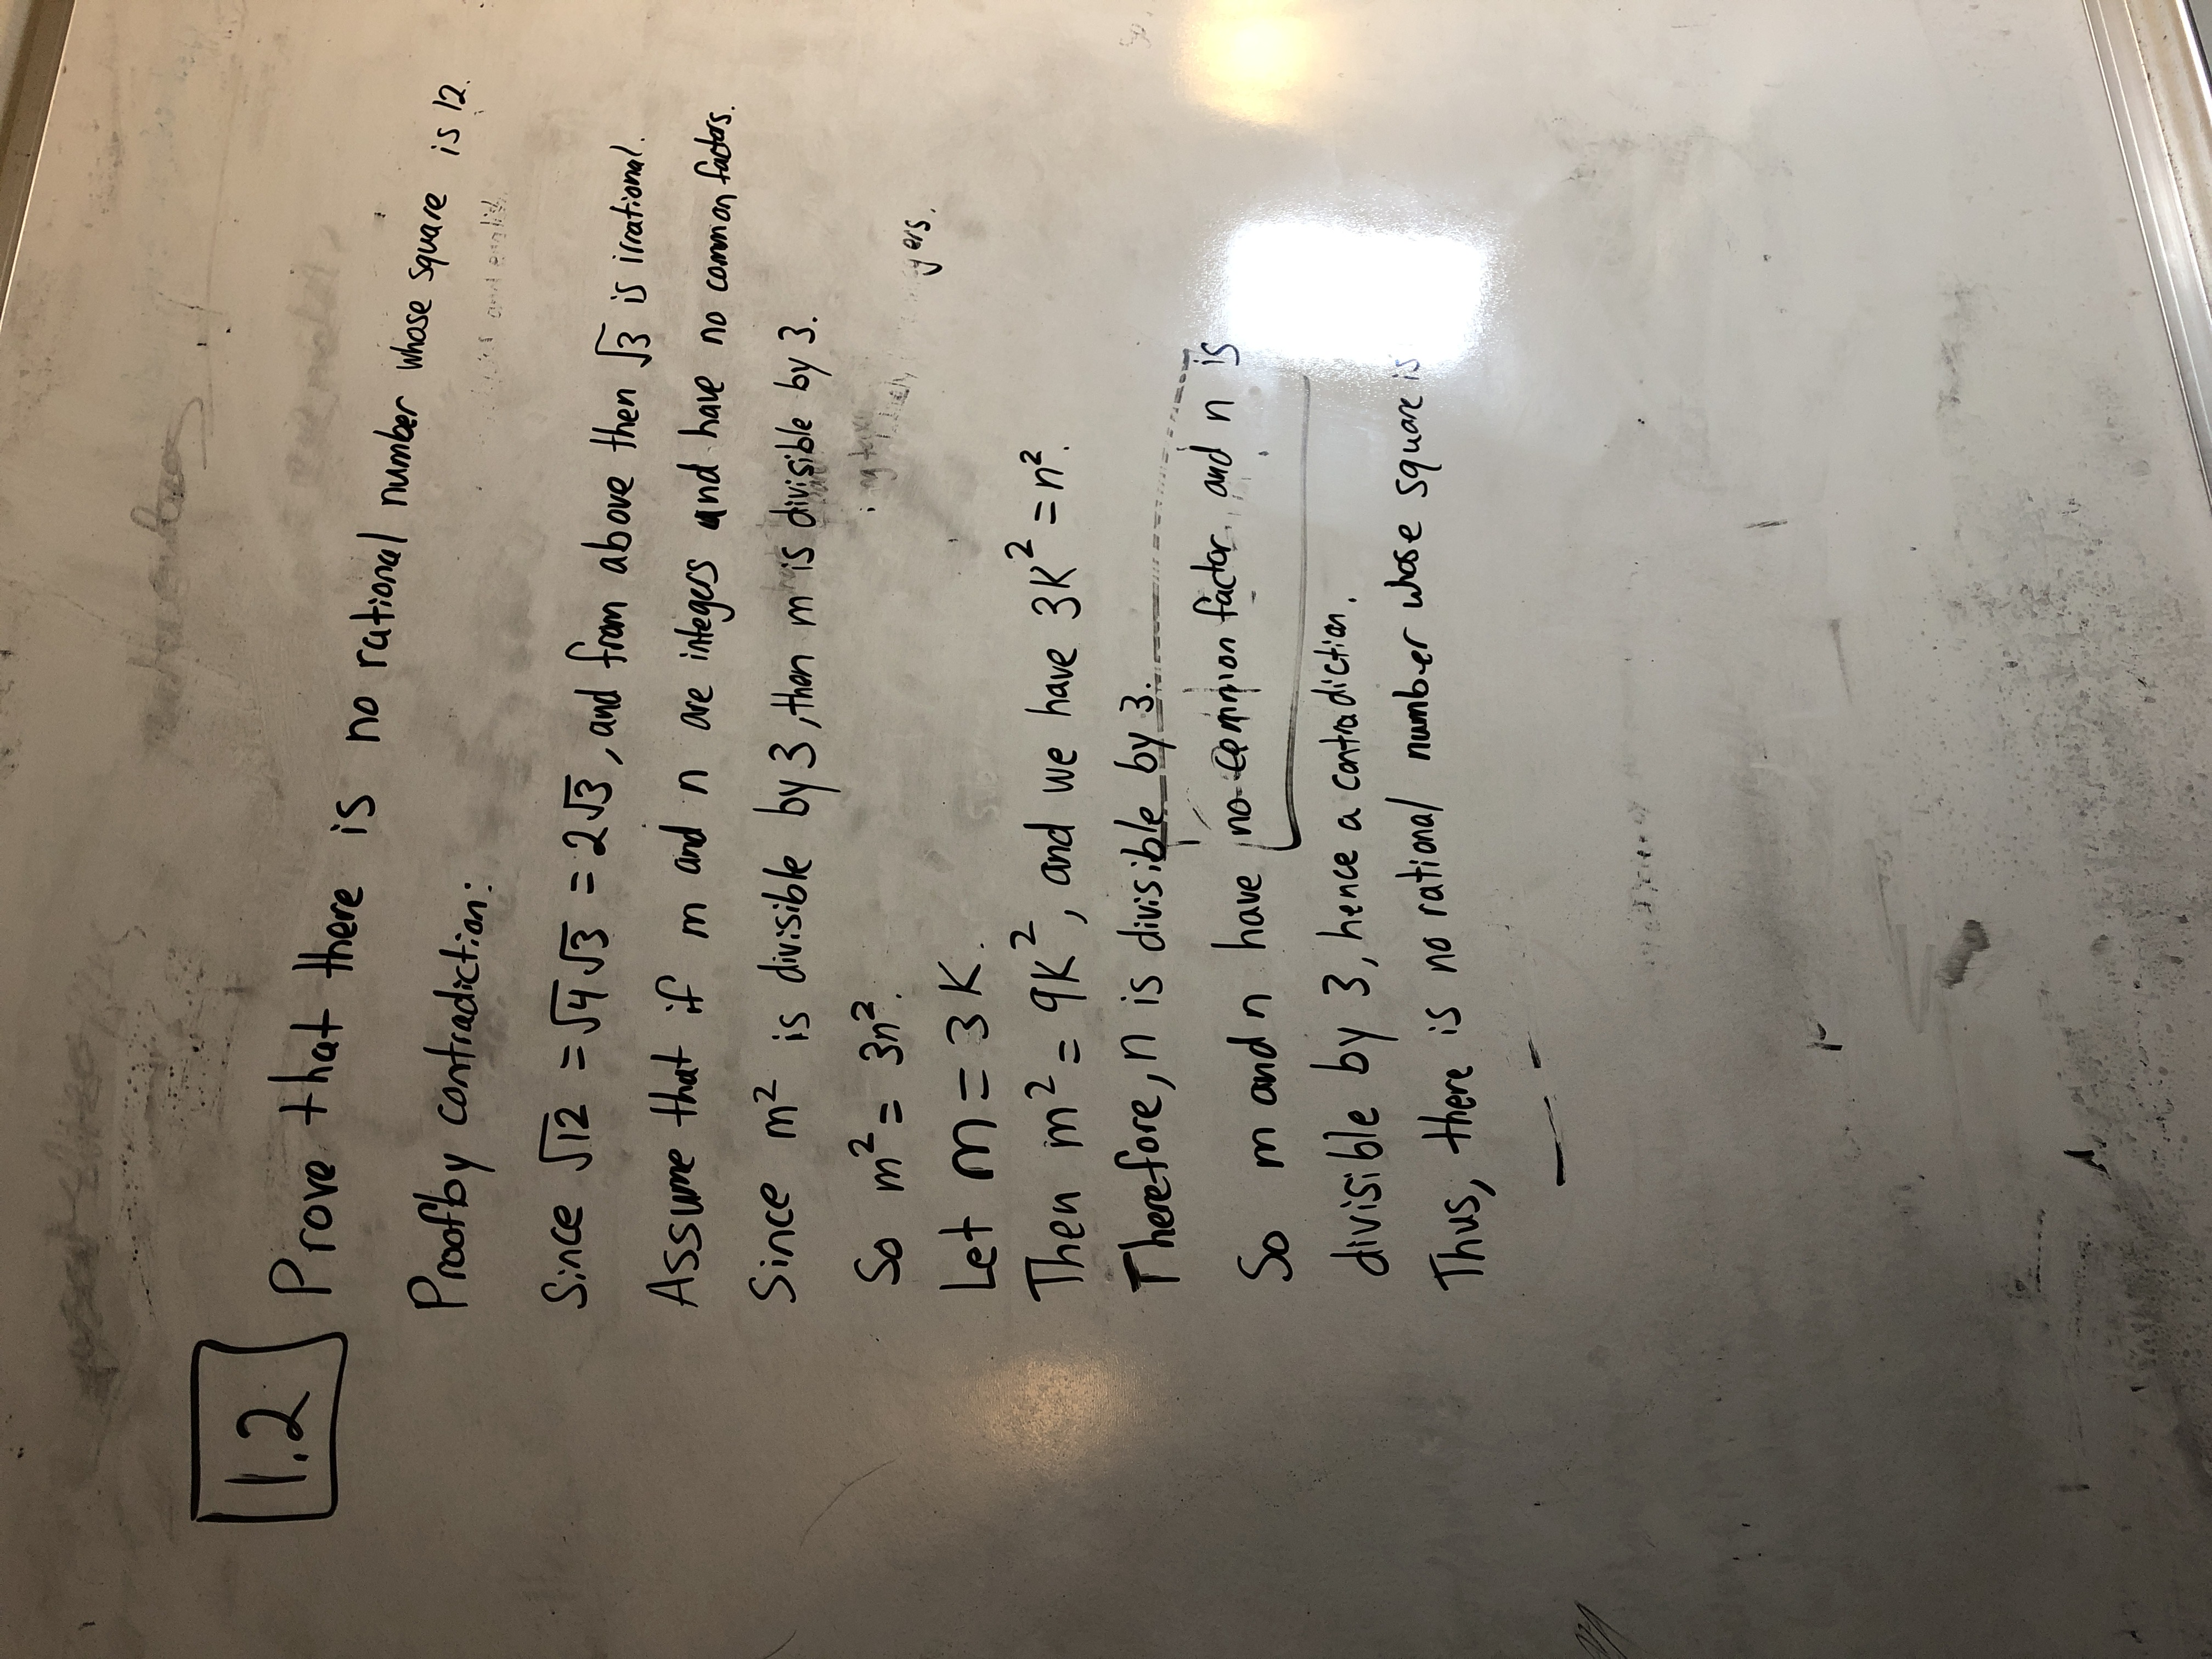
\includegraphics[angle=, origin=c,width=5 in]{Figures/IMG_1077.JPG}
\caption{Placeholder for my proofs} \label{fig:Euler_pic}\end{center}\end{figure} 

\subsection*{Baby Rudin Independent Study: Problem 10}
Suppose $z= a+bi$, $w=u+iv,$ and $a= \left(\frac{|w|+u}{2} \right)^\frac{1}{2}, b= \left(\frac{|w|-u}{2} \right)^\frac{1}{2}.$ \\ 
Prove that $z^2 =w$ if $v\geq 0$ and that $(\bar{z})^2=w$ if $v \leq 0.$ Conclude that every complex number (with one exception!) has two complex square roots. \\ 
Proof: \\ 
$z^2= (a+bi)^2= (a^2-b^2)+2abi.$\\
So, $a^2-b^2= \frac{|w|+u}{2}- \frac{|w|-u}{2}=u.$\\
Since $(xy)^\frac{1}{2}= x^\frac{1}{2} y^\frac{1}{2},$ ,$2ab= 2 \left( \frac{|w|+u}{2} \frac{|w|-u}{2}\right)^\frac{1}{2}= 2 \left( \frac{|w|^2 -u^2}{4}\right)^\frac{1}{2}.$\\
Therefore, $2ab = 2 \left( \left(\frac{v}{2} \right)^2 \right)^\frac{1}{2}.$ \\ 
So, $(x^2)^\frac{1}{2} =x$ if $x \geq 0$ and $(x^2)^\frac{1}{2}= -x$ if $x \leq 0.$ 
\\Thus, 2ab=v if $v \geq 0$ and $2ab= -v$ if $v \leq 0.$ \\ 
Hence $z^2 =w$ if $v \geq 0.$ \\ 
Then plugging in b with -b, we find that $( \bar{z})^2=w$ if $v \leq 0.$ \\ 
Then plugging in b with -b , we find that $(\bar{z})^2=w $ if $v \leq 0. $ \\ 
Thus, every non-zero complex number has (at least) two complex square roots. Hence it is proved. 


\subsection*{Baby Rudin: Independent Study Problem 12}

Here as follows is a proof setting up for Cauchy Schwartz inequality. Ideally, I would like to type set theorem 1.33 for reference. 
\section*{Problem 12}
If $z_1,...,z_n$ are complex, prove that \\
\\$|z_1 +z_2 + ... +z_n| \leq |z_1| + |z_2| + ... +|z_n|.$ \\ 
Proof by induction: \\ 
Base case:
Since in Theorem 1.33, $|z+w| \leq |z|+|w|.$ \\ 
Then when n=2 $|z_1+z_2| \leq |z_1|+|z_2|$.
\\ 
Inductive Step:
\\ 
$|z_1+z_2 + ... +z_n|= |(z_1 +z_2 + ... + z_{n-1}) +z_n|.$ \\ 
$|z_1+z_2 + ... +z_n|\leq |z_1 +z_2 + ... + z_{n-1} +z_n|.$ \\ 
Hence, $|z_1+z_2 + ... +z_n| \leq |z_1| +|z_2| + ... + |z_{n-1}| +|z_n|$ is proved by induction. \\ 
\begin{figure}[ht]\begin{center}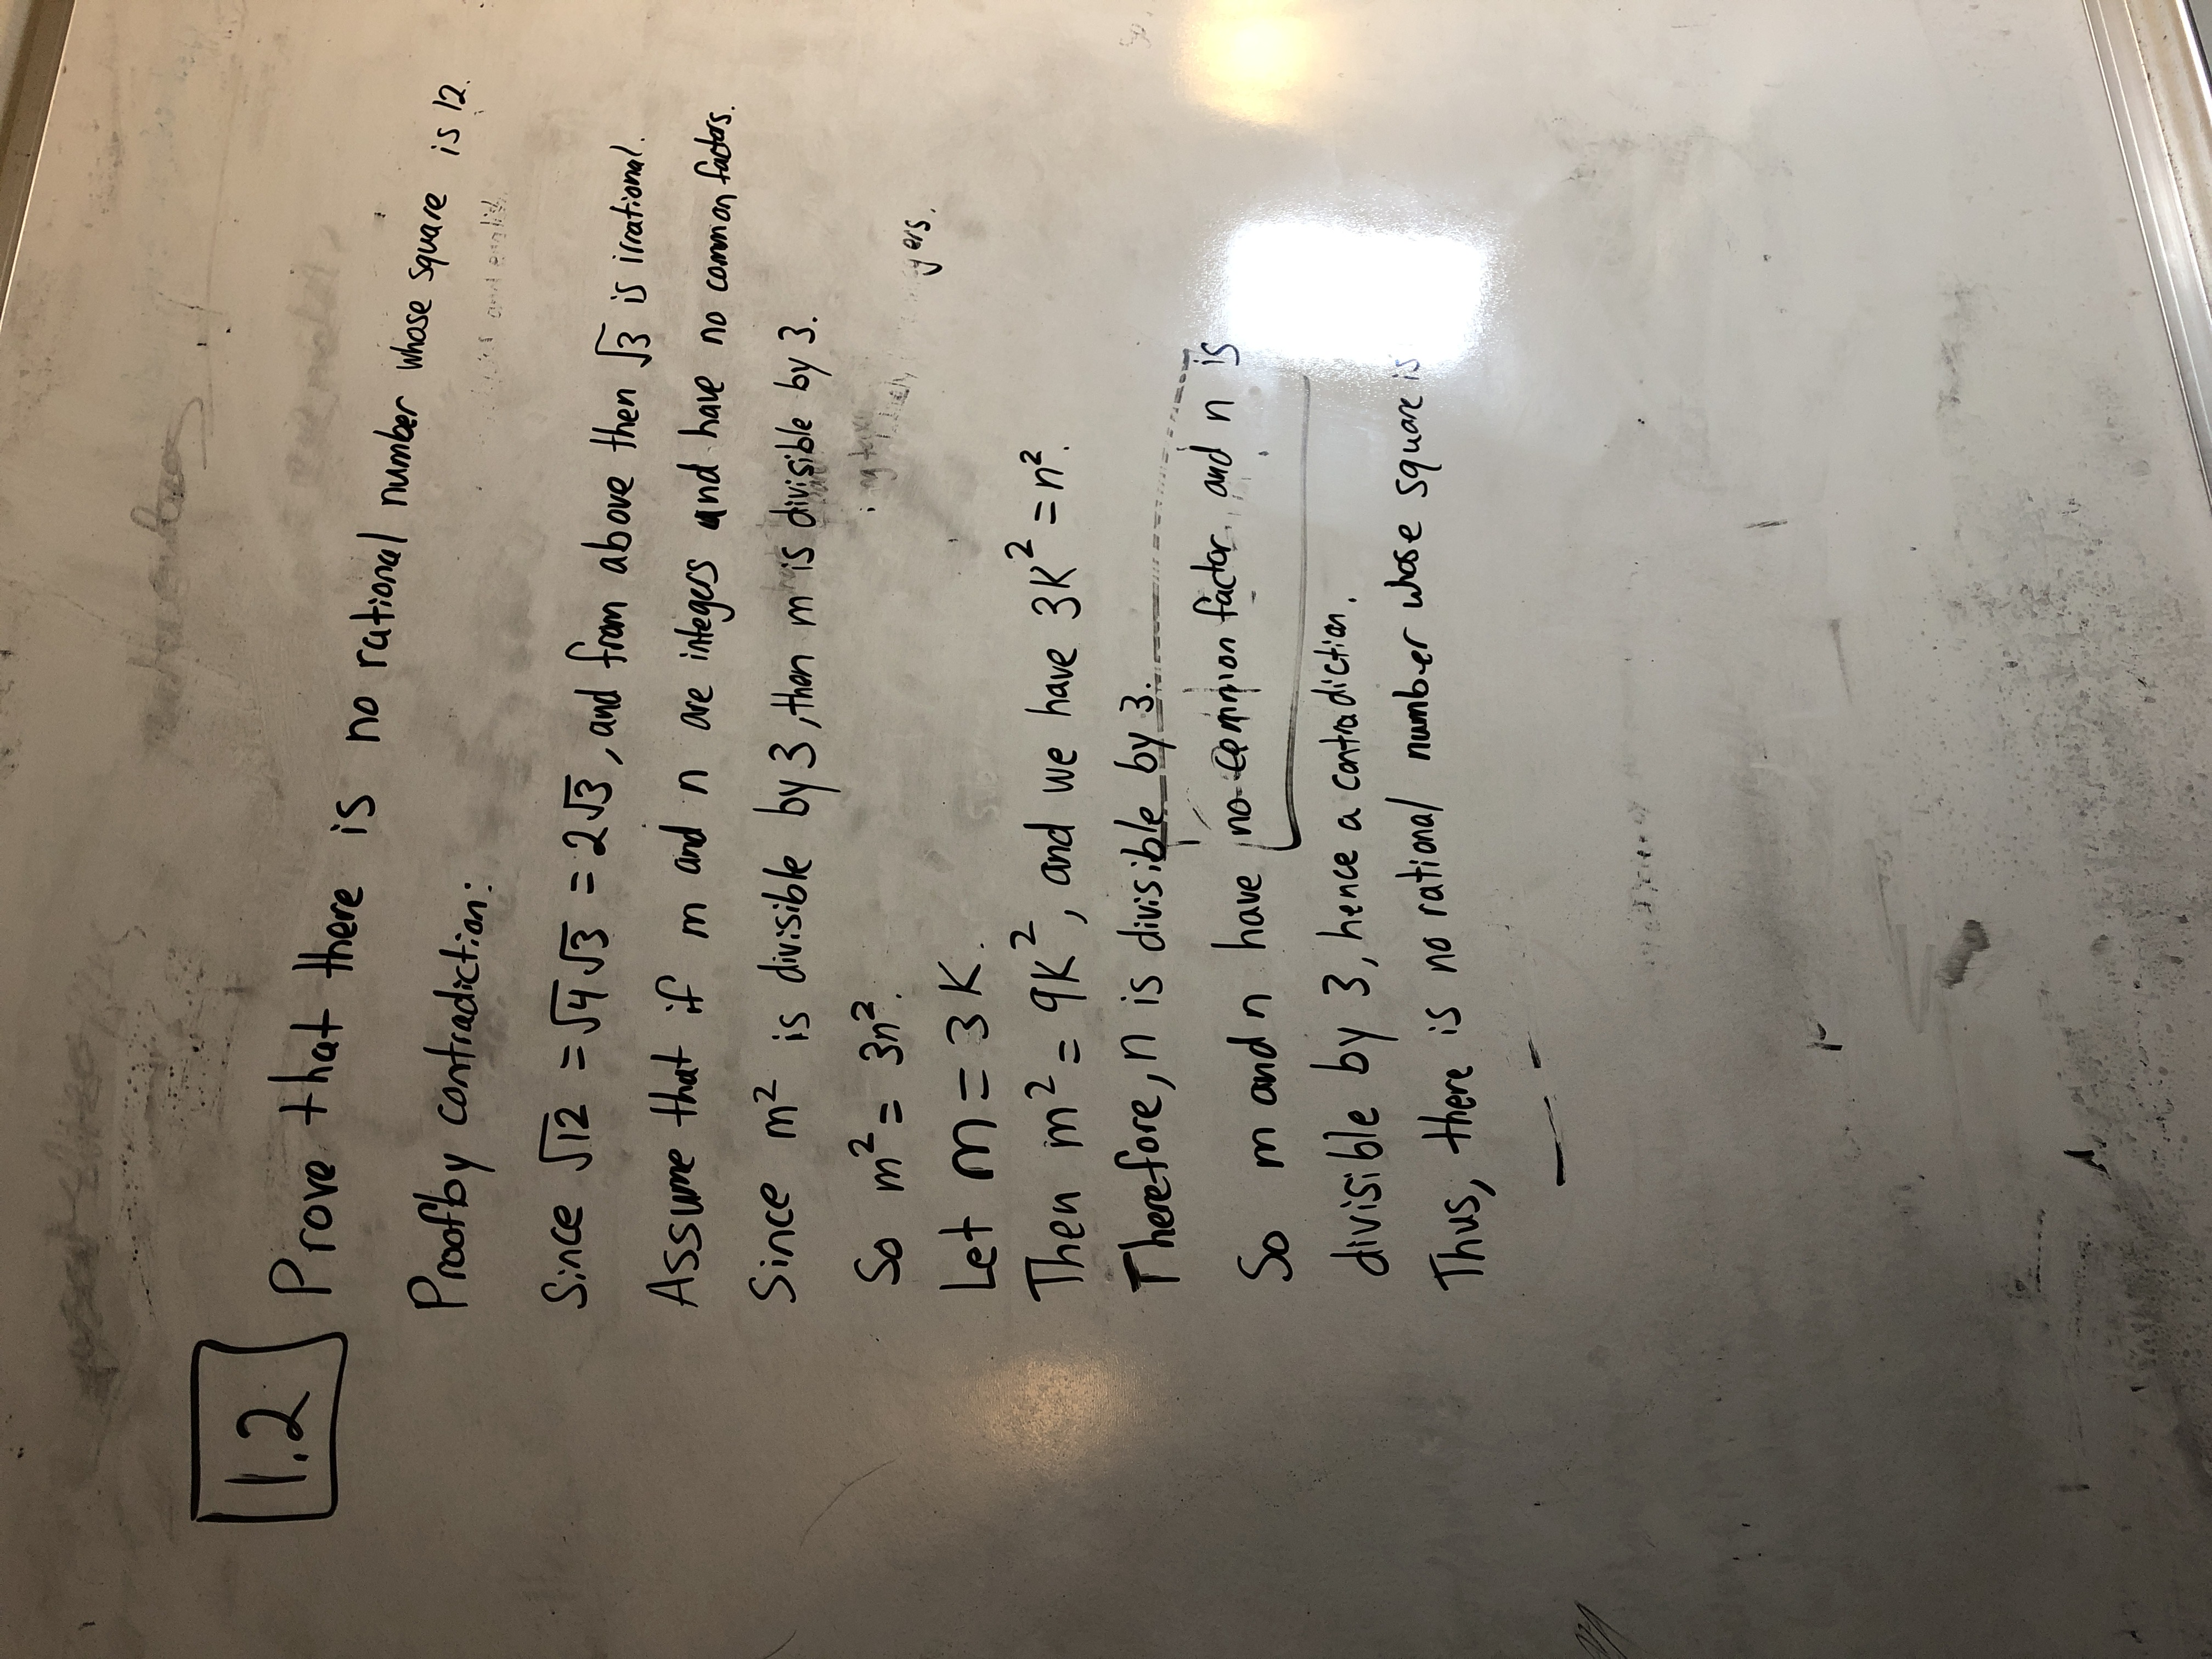
\includegraphics[angle=, origin=c,width=5 in]{Figures/IMG_1077.JPG}
\caption{Placeholder for my proofs} \label{fig:Euler_pic}\end{center}\end{figure} 

\newpage 
\subsection*{Baby Rudin Independent Study: Problem 13}
If x,y are complex, prove that $||x|-|y|| \leq|x-y|.$ \\
Proof: \\ 
Since x= x-y+y, by definition of the triangle inequality $|x| \leq |x-y|+y$, so $|x|-|y| \leq |x-y|.$ \\ 
So $|y|-|x| \leq |x-y|$. \\ 
Since $|x| - |y|$ is in the set of real numbers, then $||x|-|y|$ or $||x|-|y||= |y|-|x|.$ \\
Thus, $||x|-|y|| \leq |x-y|$. Hence it is proved. 
\begin{figure}[ht]\begin{center}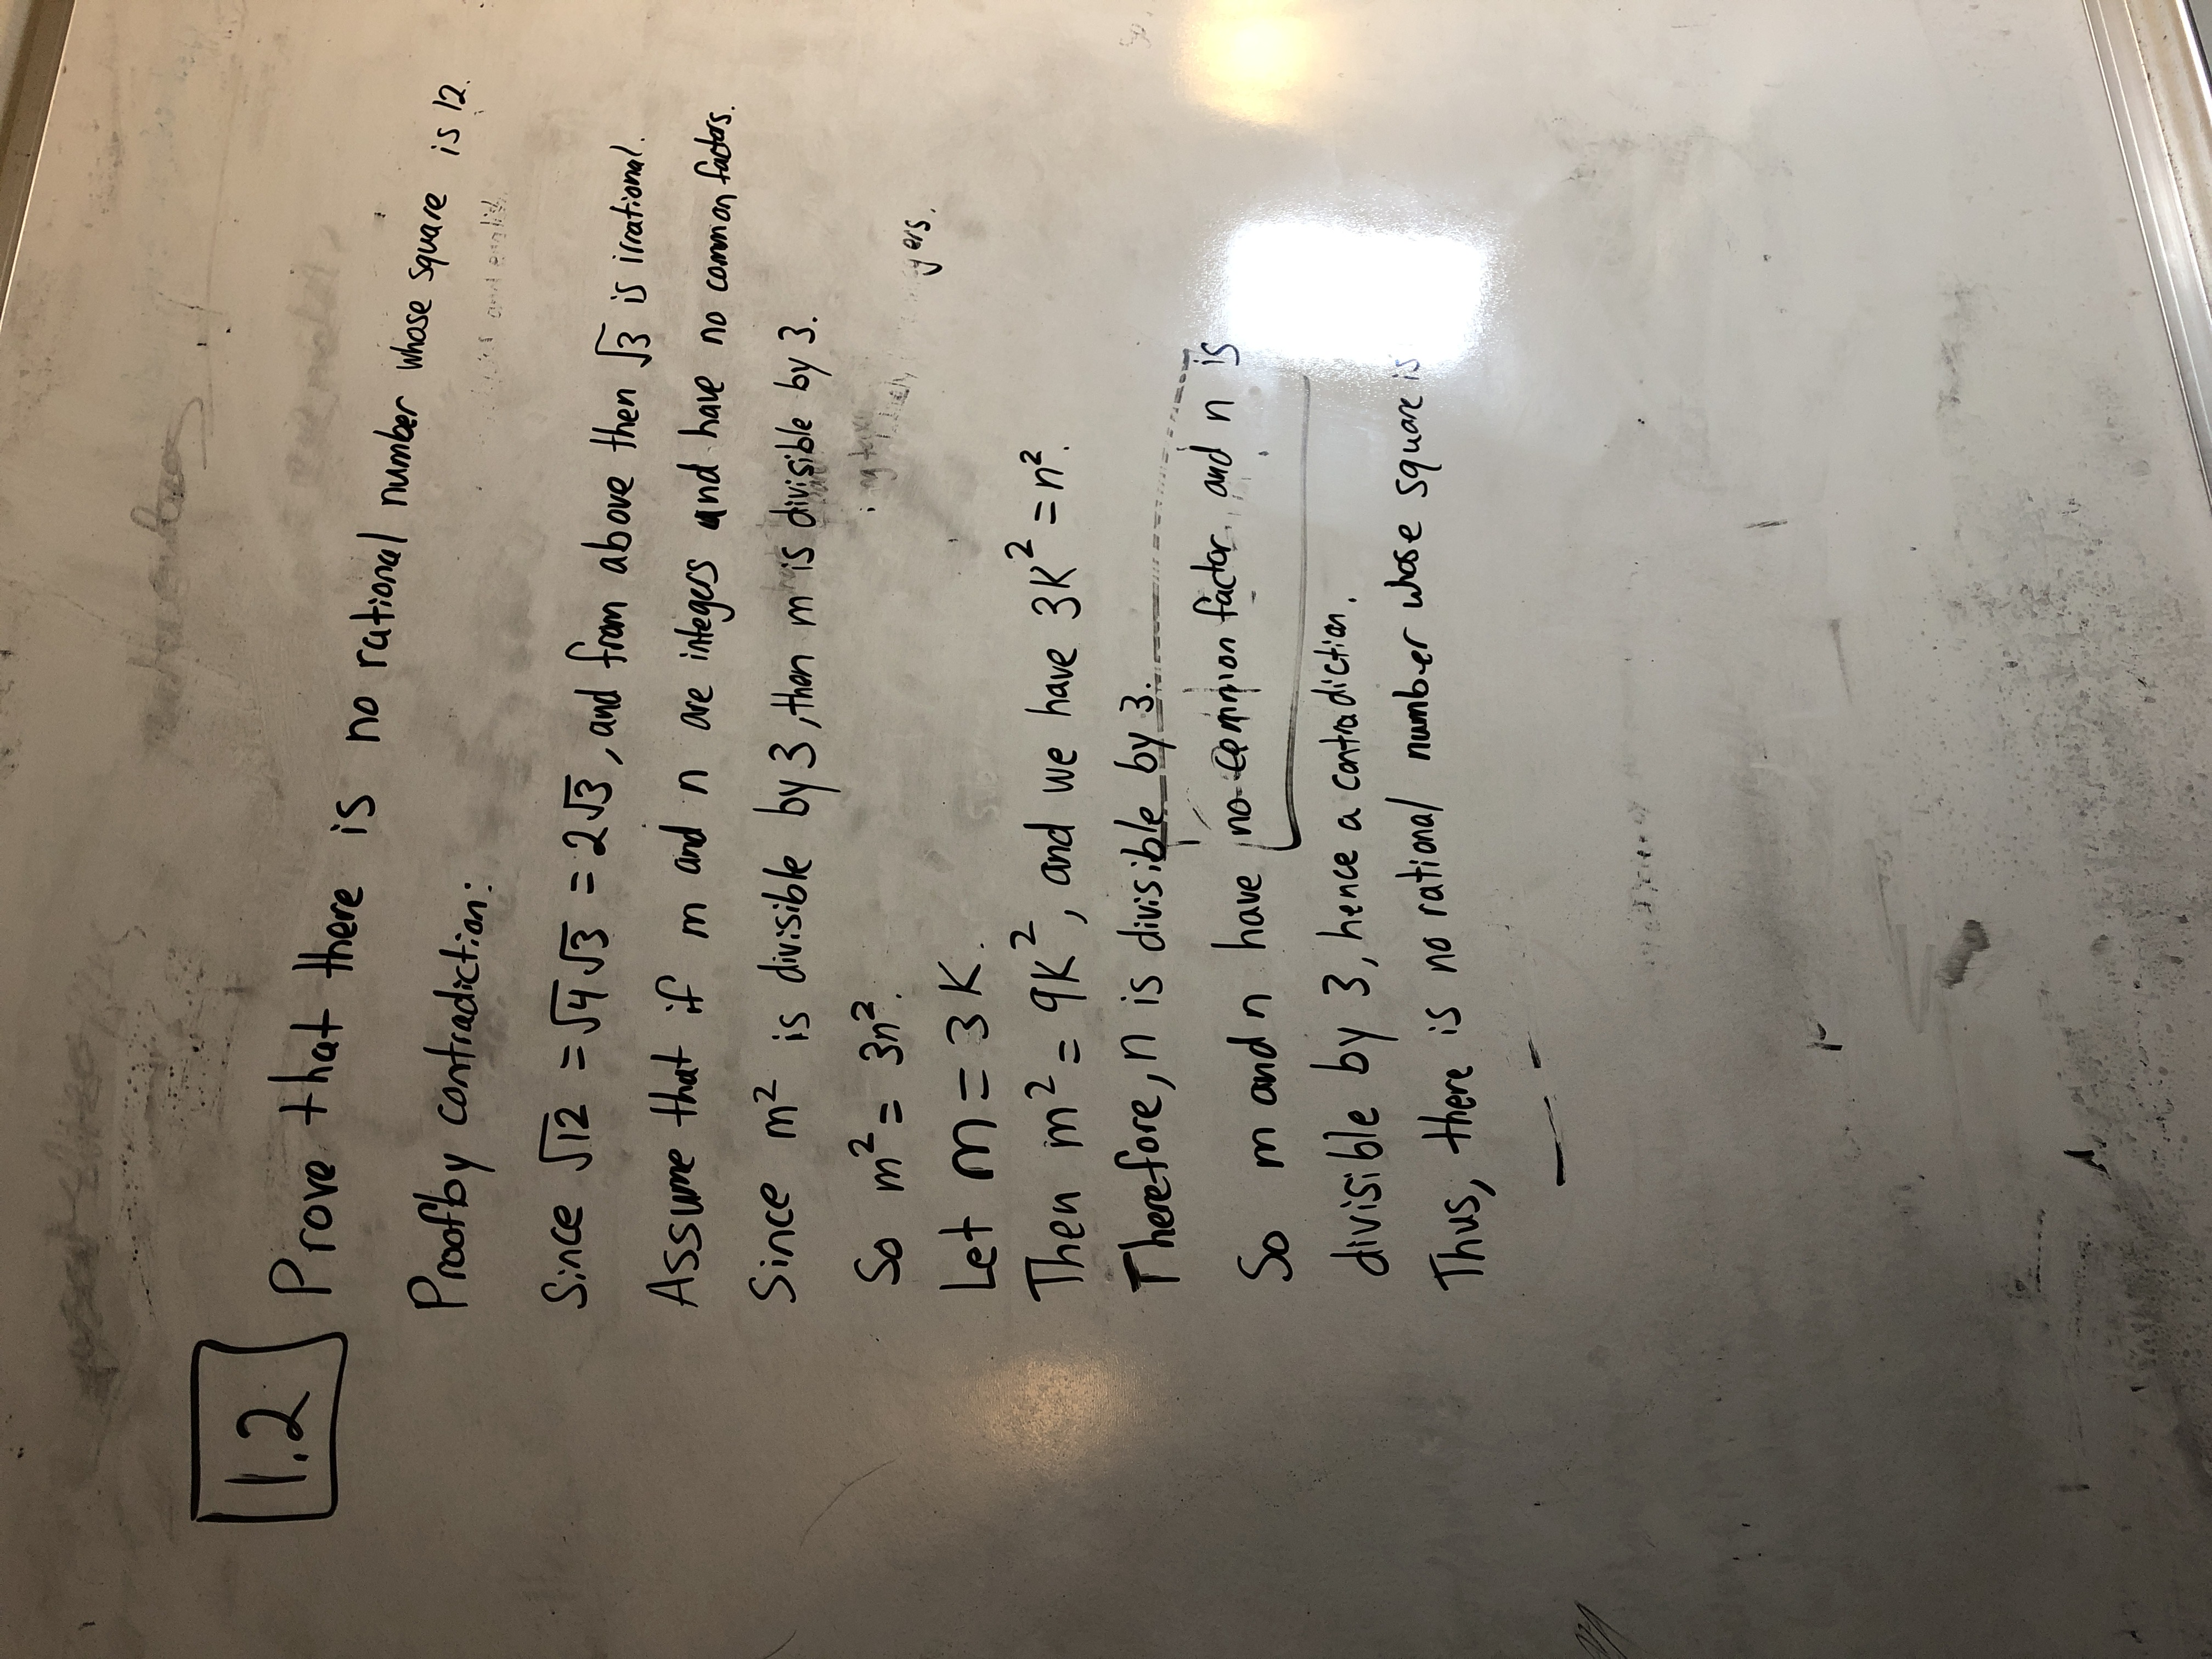
\includegraphics[angle=, origin=c,width=5 in]{Figures/IMG_1077.JPG}
\caption{Placeholder for my proofs} \label{fig:Euler_pic}\end{center}\end{figure} 
\newpage
Grade Problem 2.1 and 2.3.  
\subsection*{Problem 1.16}
Suppose $k \geq 3, x,y,\in R^k, |x-y|=d>0,$ and $r>0.$ \\ Prove: 
(a)If $2r>d$, there are infinitely many z $\in R^k$ such that $|z-x|=|z-y|=r.$ \\ 
(b) If $2r = d,$ there is exactly one such z. \\ 
(c) If $2r < d,$ there is no such z. \\ 
How must these statements be modified if k is 2 or 1? \\ 
Proof: \\ 
(a) Let w be any vector where: \\ 
$w \cdot (x-y)=0,$ \\ 
$|w|^2 = r^2 - \frac{d^2}{4}.$ \\ 
%From linear algebra it is known that all but one of the components of a solution w of the first equation can be arbitrary. \\
%The remaining component is then uniquely determined.Also, if w is any non-zero solution of the first equation, there is a unique positive number t such that tw satisfies both equations. (For example, if $\x_1 \neq y_1, $ the first equation is satisfied whenever $z_1 =\frac{z_2(x_2-y_2)+ \dots + z_k(x_k-y_k)}{y_1-x_1}.$ \\ 
%If $(z_1, z_2, \dots, z_k)$ satisfies this equation, so does $(tz_1, tz_2, \dots tz_k)$ for any real number t.) Since at least two of these components can vary independently, we can find a solution with these components having any prescribed ratio. This ratio does not change when we multiply by the positive number t to obtain a solution of both equations. 
Since there are infinitely many ratios, there are infinitely many distinct solutions. For each such solution w the vector z= $\frac{1}{2}x + \frac{1}{2}y + w$ is a solution of the required equation. For \\
$|z-x|^2= |\frac{y-x}{2}+w|^2$ \\ 
$|z-x|^2= |\frac{y-x}{2}|^2 +2w \cdot \frac{x-y}{2}+|w|^2$ \\ 
$|z-x|^2= \frac{d^2}{4}+0 +r^2 -\frac{d^2}{4}$ \\ 
$|z-x|^2 = r^2,$ \\
$|z-y|^2=r^2.$ \\ 
(b) The triangle inequality proof demonstrates that $2r=d$ only is true if it is equal in the Schwartz inequality.\\ Then one of the two vectors is a scalar multiple of the other one.\\ Furthermore, the scalar must be nonnegative. 
\\Next, $|x-y|=d=|x-z|+|z-y|.$ \\ 
Hence, there is a nonnegative scalar t such that $x-z =t(z-y).$ \\ 
So, the above equation leads to t=1. \\ 
So z is uniquely determined as $z= \frac{x+y}{2}.$ \\ 
(c) The triangle inequality is contradicted if z=$2r<d$. Then we would have $|x-y|=d>2r =|x-z|+|z-y|.$ When k=2, there are exactly 2 solutions when $2r>d$. When k=1, there are no solutions when $2r>d$. \\ 

\begin{figure}[ht]\begin{center}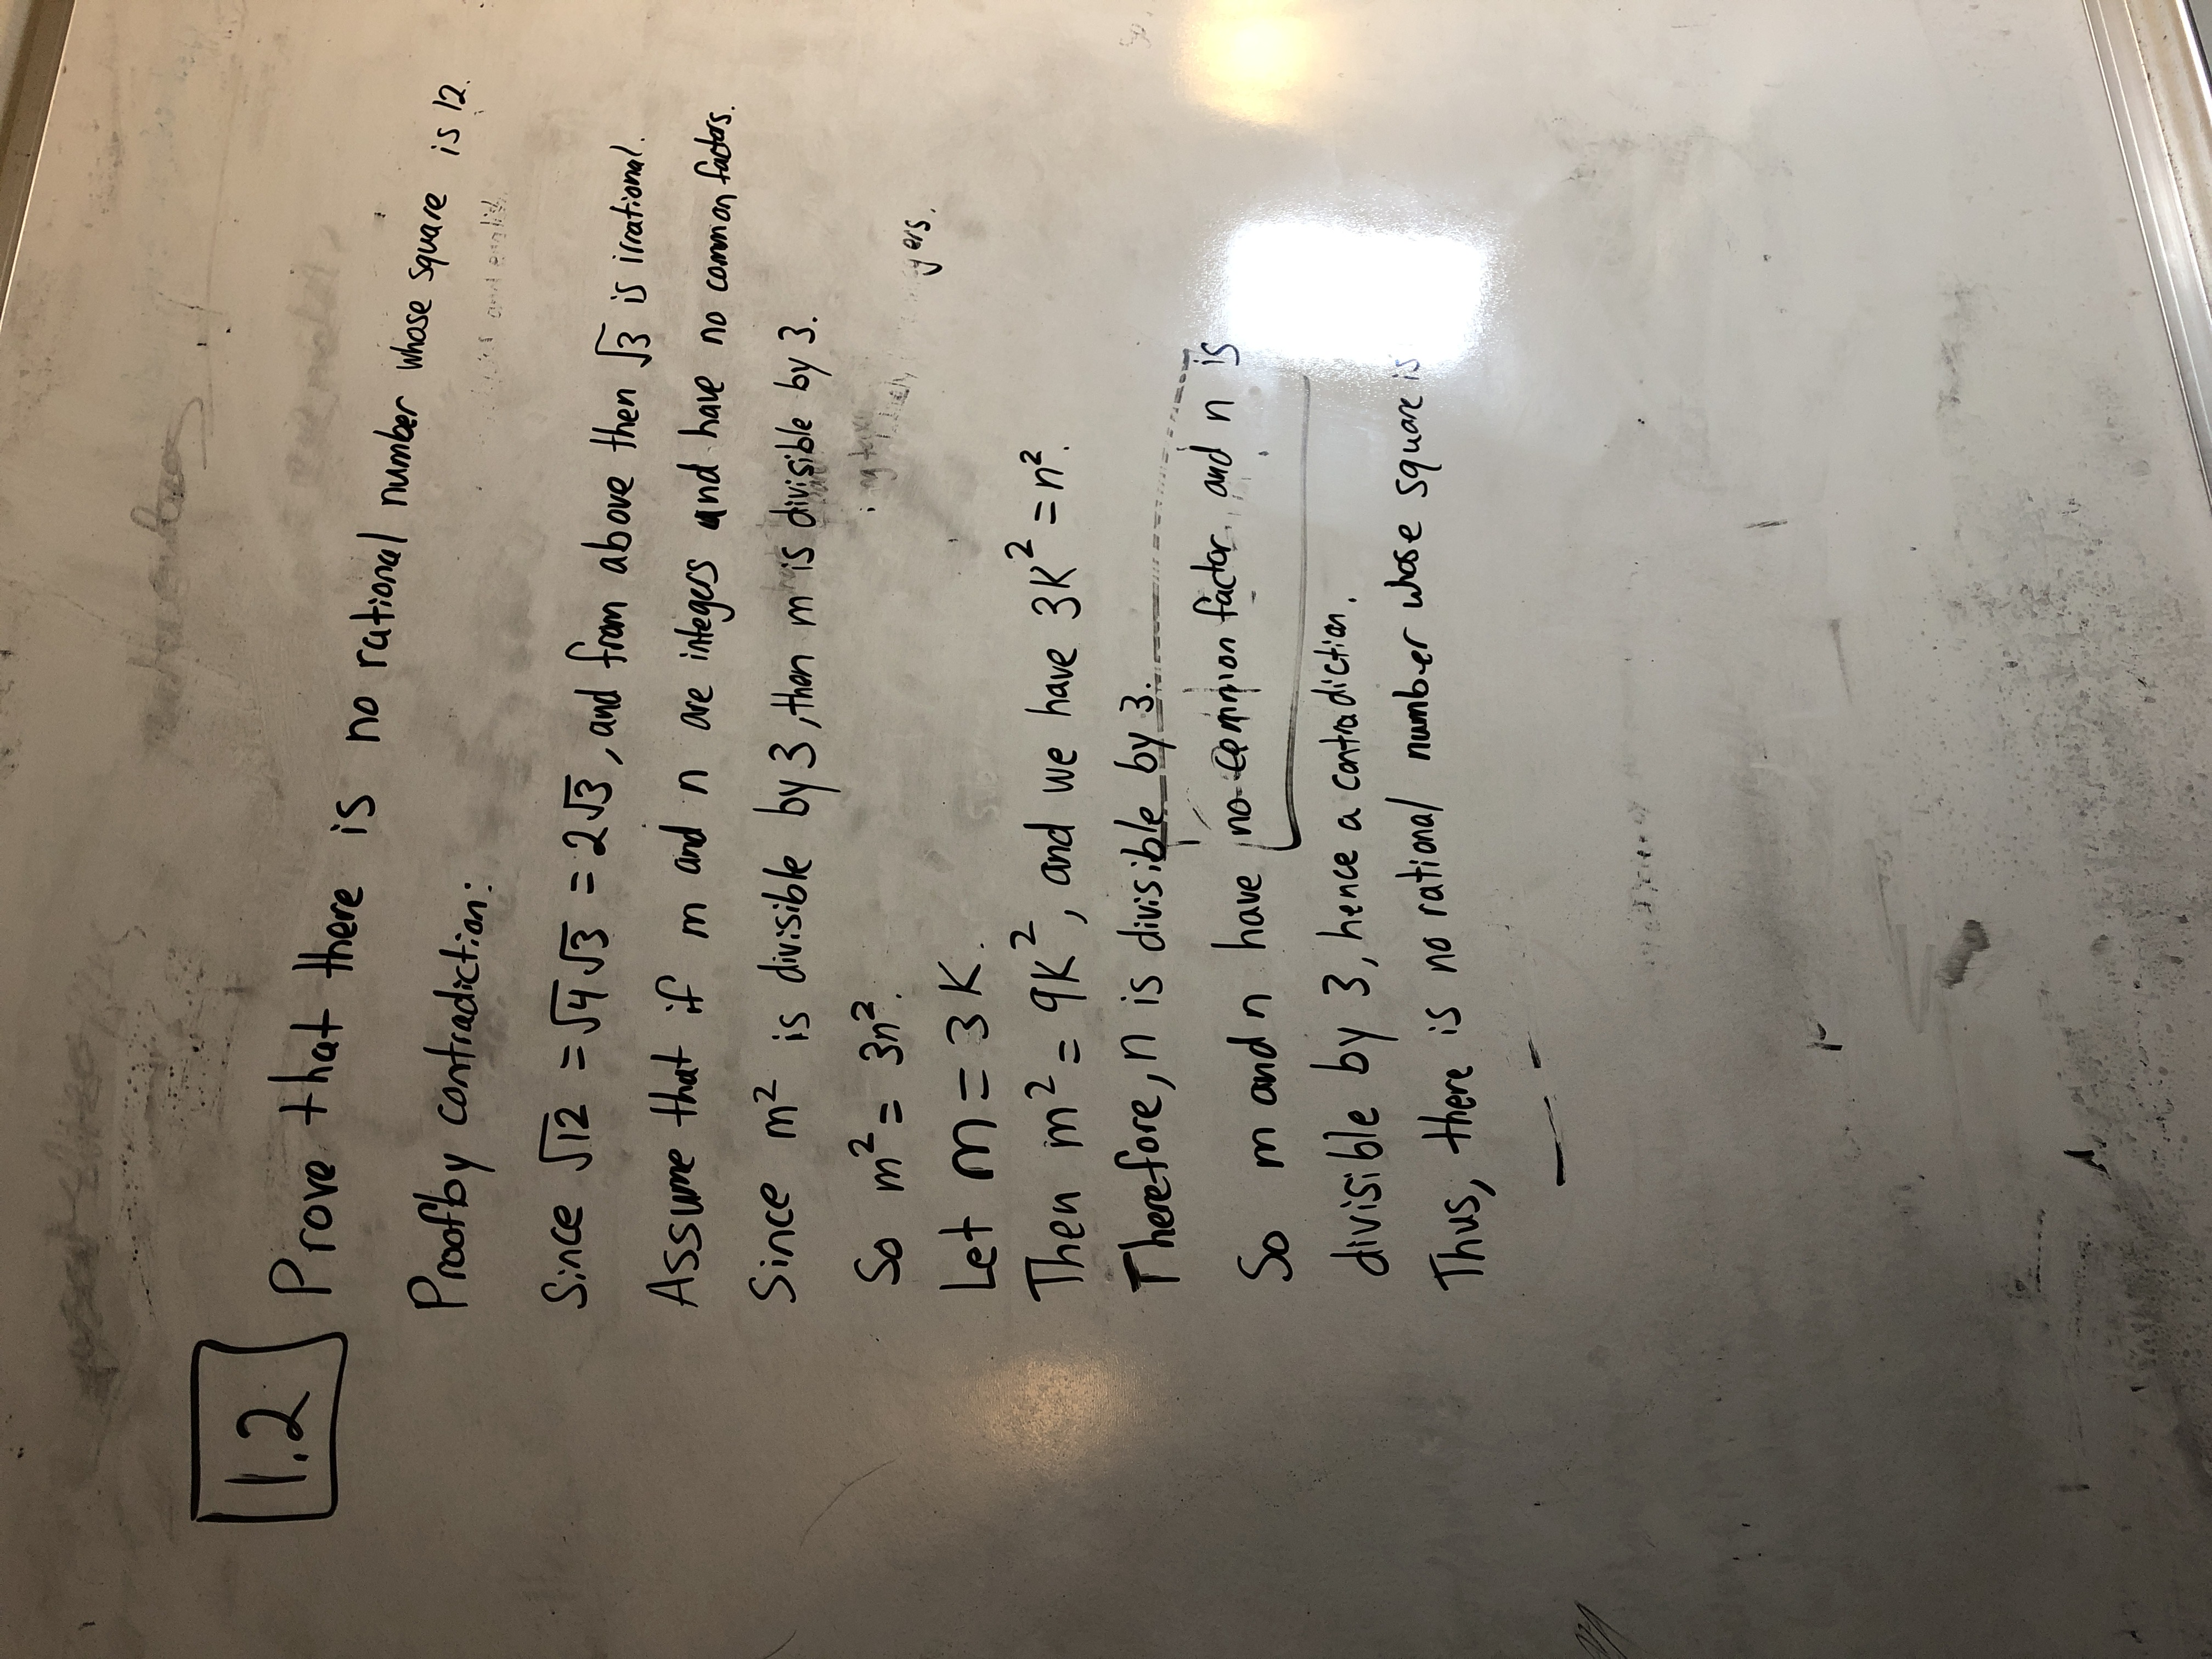
\includegraphics[angle=, origin=c,width=5 in]{Figures/IMG_1077.JPG}
\caption{Placeholder for my proofs} \label{fig:Euler_pic}\end{center}\end{figure} 
\newpage
\subsection{Problem 1.18}
If $k \geq 2$ and $x \in R^k,$ prove that there exists $y \in R^k$ such that $y \neq 0$ but $x \cdot y =0.$ Is this also true if k=1? \\ 
Proof: \\ 
If x has any components equal to 0, then y can be taken to have the corresponding components equal to 1 and all others equal to 0.\\
If all the components of x are nonzero, y can be taken as $-x_2,x_1,0, \dots,0).$ \\
Since the product of two nonzero real numbers is nonzero then this is not true when k=1, \\ 
\\
\begin{figure}[ht]\begin{center}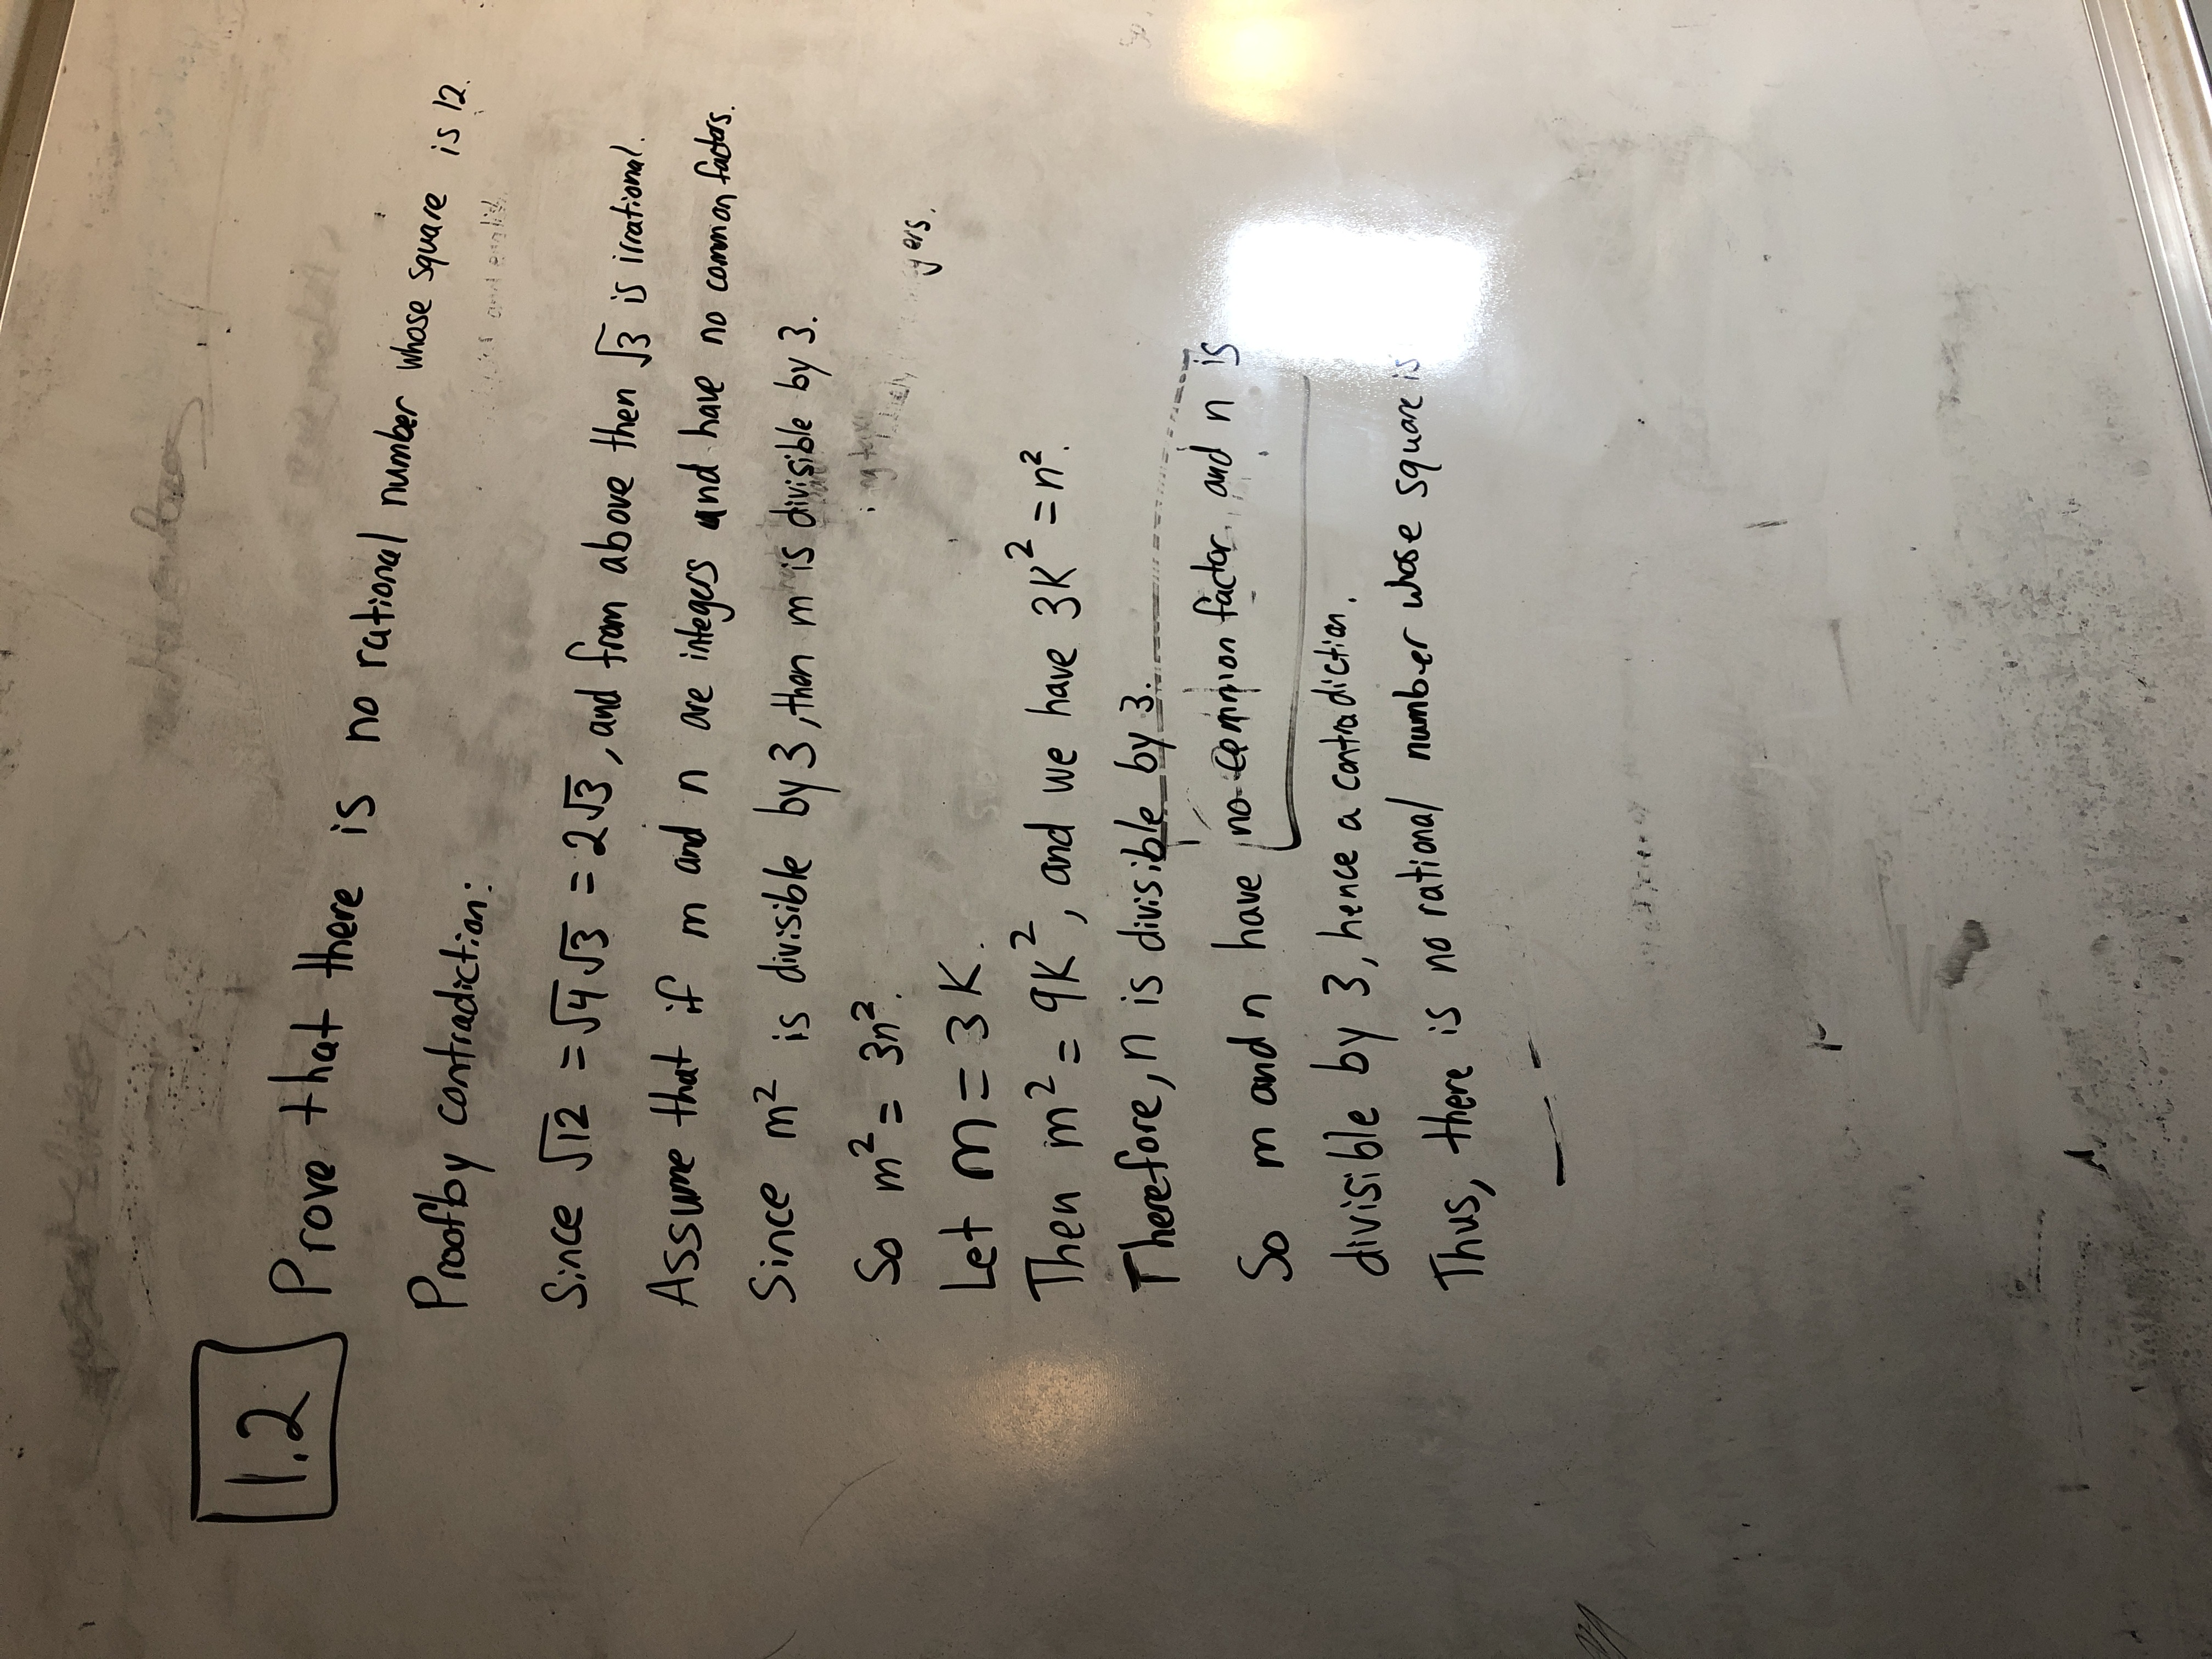
\includegraphics[angle=, origin=c,width=5 in]{Figures/IMG_1077.JPG}
\caption{Placeholder for my proofs} \label{fig:Euler_pic}\end{center}\end{figure} 



\section{The First Compilation}

\subsection*{Me Pontificating}

\subsubsection*{Questions to pay attention to and ask Dr. Ross about This is Due by Monday}
\subsubsection*{What to talk to Dr. O'Shaugnessy about}
Random walks and what not 
\section{Finite, Countable, Uncountable Sets}
For each of the following sets, determine whether the set is finite, countable, or uncountable. Prove your claims. \\
\subsection{The real numbers that can be expressed as infinite sums}

\subsection{The set of all possible Soduku Puzzles}


\subsection{The real numbers that can be expressed as infinite sums something something binary numbers}


\subsection{All of the pages in all of the books that have ever been printed}

\subsection{Natural Numbers one}
The set of all functions whose domain is $\N$ and whose range is the finite set $\{0,1,2,3,4,5,6,7,8,9\}$

\subsection{The set consisting of all binomial coefficients}

\section*{Inner Product and Dot Product Problem just think about the tensor product...get it done so you can go back to your research and a real 200k income so you can carry out your dreams}\\ 
\textbf{In other news why I should care about this other than for my gpa and to continue my research and be off of probation due to my stress associated with my family during a pandemic...photons and how the dot product is 0 since they are massless particles the dot product as relates to the general relativity minkowski metric }\\
In $R^k$consider the inner product- an inner product that is not the usual dot product-that is defined, for vectors $\Vec{x}=(x_1,x_2,...,x_k)$ and $\Vec{y}=(y_1,y_2, ..., y_k)$ by the formula \\ 
$\Vec{x} * \Vec{Y}= \Sigma_{j=1}^{k}c_j x_j y_j$ \\ 
where $c_1, c_2, ... c_k$ are positive real numbers. We define a vector norm, $||\Vec{x}||_{*}=\sqrt{\Vec{x}*\Vec{x}}$ and we define a function $d_*(\Vec{x}, \Vec{y})=||\Vec{x}-\Vec{y}||_*=\sqrt{(\Vec{x}-\Vec{y}*(\Vec{x}-\Vec{y})}$ \\ 
Now we have two different inner products, the one we just introduced, $\Vec{x}*\Vec{y}=\Sigma_{j=1}^k c_{j}x_{j}y_{j}$ with its associated norm, $||\Vec{x}||_*=\sqrt{\Vec{x}*\Vec{x}}$ and the metric, $d_{*}(\Vec{x},\Vec{y})=||\Vec{x}-\Vec{y}||_{*}=\sqrt{(\Vec{x}-\Vec{y})*(\Vec{x}-\Vec{y})}$ and the standard inner product, $\Vec{x}\dot\Vec{y}=\Sigma_{j=1}^{k}x_jy_j$ with its associated norm $||\Vec{x}||_2 = \sqrt{\Vec{x}\dot \Vec{x}}$ and the metric $|\Vec{x}-\Vec{y}|=\sqrt{(\Vec{x}-\Vec{y}\dot \Vec{x}-\Vec{y})}$ \\ 



\section{Finite, countable, or uncountable sets}
For each of the following sets, determine whether the set is finite, countable, or uncountable. Prove your claims. \\ 
\subsection{Infinite sums}
The real numbers that can be expressed as infinite sums of the form $x= \sum_{j=k}^\infty q^{j}$ where k is a nonnegative integer and q is a rational number. 
\\ 
It is countable. \\ 


The novice proof: 

It is countable since 
\subsection{Sudoku}
The set of all possible Sudoku puzzles.
\\ 
It is countable. The number of different puzzles would be a large number for all the different permutations, but it would be finite and countable. \\ 


\subsection{Another infinite sum} 
The real numbers that can be expressed as infinite sums of the form \\ 
$x= \sum_{j=0}^\infity b_j2^{-j}$ where each $b_j$ is either 0 or 1. \\ 

This would be uncountable. 
\subsection{Book Pages}
All of the pages in all books that have ever been printed. 
\\ 
It is a growing number. It is countable since it could be feasible to calculate this number, but it is not realistic since books may have been burned so since the word ever is used it may not be that way. 

\subsection{Domain and range}
The set of all functions whose domain is the Natural numbers and whose range is the finite set ${0,1,2,3,4,5,6,7,8,9}.$
This would be uncountable. 
\subsection{Binomial Coefficients}
The set consisting of all binomial coefficients.
\\ 
This would be countable since the permutation would be the natural numbers cross the natural numbers. 
\section{Inner Product}
In $R^k$ consider the inner product- an inner product that is not the usual dot product-that is defined, for vectors $\vec{x}=(x_1, x_2,..., x_k)$ and $\vec{y}=(y_1,y_2,...,y_k)$ by the formula \\ 
$\vec{x}*\vec{y}= \sum_{j=1}^k c_j x_j y_j$ \\ where $c_1,c_2,...,c_k$ are positive real numbers. We define a vector norm, $||\vec{x}||_{*}=\sqrt{\vec{x}*\vec{x}}$ and we define a function $d_*(\vec{x},\vec{y})=||\vec{x}-\vec{y}||_{*}=\sqrt{(\vec{x}-\vec{y}*(\vec{x}-\vec{y}}.$\\ 
Now we have two different products, the one we just introduced, $\vec{x}*\vec{y}= \sum_{j=1}^k c_j x_j y_j$, with its associated norm, $||\vec{x}||_{*}=\sqrt{\vec{x}*\vec{x}}$ and the metric, $d_*(\vec{x},\vec{y})=||\vec{x}-\vec{y}||_{*}=\sqrt{(\vec{x}-\vec{y}*(\vec{x}-\vec{y}}$ and the standard inner product, $\vec{x}\cdot \vec{y}= \sum_{j=1}^k x_j y_j$ with its associated norm $||\vec{x}||_{2}=\sqrt{\vec{x}\cdot \vec{x}}$ and the metric $\vec{x}-\vec{y}=\sqrt{(\vec{x}-\vec{y})\cdot (\vec{x}-\vec{y})}$. \\ 
\subsection{Schwartz Inequality}
State and prove the analog of the Schwartz inequality for $\vec{x}*\vec{y}.$ \\ 
Theorem 1.35. \\ 
If $a_1,...,a_n$ and $b_1,...,b_n$ are complex numbers then $|\sum_{j=1}^n a_j \bar{b_j}|^2 \leq \sum_{j=1}^n |a_j|^2 \sum_{j=1}^n |b_j|^2.$ \\ 

\subsection{Positive real numbers M} 
Prove that there are positive real numbers M and m such that for all vectors $\vec{x}$ and $\vec{y}$ \\ 
$|\vec{x}\cdot \vec{y}\leq M ||\vec{x||_{*}}||\vec{y||_{*}}$ and \\ $m|\vec{x}*\vec{y}\leq ||\vec{x}||_2||\vec{y}||_2$ and find the largest such m and the smallest such M. \\ 
\subsection{c_j = j} 
For k=5, consider the case in which $c_j=j.$ For an arbitrary $\vec{x}=(x_1,x_2,...,x_k),$ find a non-zero $\vec{y}=(y_1,y_2,...,y_k)$ such that $\vec{x}*\vec{y}=0.$ \\ 
\subsection{If c was not positive} 
If not all $c_1,c_2, ...,c_k$ were positive, $d_{*}(\vec{x}, \vec{y})$ would no longer be a metric. Why? 
\subsection*{Metric Space}
Let X be a metric space. A subset A is said to be dense in X if $\bar{A}=X,$ that is, if the closure of A is X. Prove that the following statements are equivalent; that is, prove that if any one of them is true they are all true:\\ 
The set A is dense in X. \\ 
The only closed set that contains A is X. \\ 
There is no non-empty open set that is disjoint from A. \\ 
The set A intersects every neighborhood. \\ 
\subsection*{Reference:Definition 2.45 Rudin}
Two subsets A and B of a metric space X are said to be separated if $A \cap \bar{B}$ and $B \cap \bar{A}$ are both empty, that is, if A is disjoint from the closure of B and B is disjoint from the closure of A. A set E in X is said to be connected if it is not the union of two non-empty separated sets. This is just Definition 2.45 in Rudin. \\ 
\subsection{Convex Set}
Prove that every convex set in $R^k$ is connected. \\ 
Definition 2.17 \\ 
We call a set $E \subset R^k$ convex if $\lambda x + (1- \lambda) y \in E$ whenever $x \in E,$ $y \in E,$ and $ 0< \lambda <1.$
\subsection{Two Subsets are separated}
Consider this claim: Two subsets A and B of a metric space X are separated if and only if $\bar{A} \cap \bar{B}$ is empty. If it's true, prove that it's true; if it's false, prove that it's false. \\ 
\section{Uncountable Collection}
Give an example of an uncountable collection of disjoint closed sets in $R^2$ \\ 
$\cup_{x \in R^2} x$
\section{Prove that there is a finite collection}
Let K be a compact subset of a metric space X. Suppose that $F_{\beta}$ is a collection of closed sets contained in K and that $\cap_{\beta} F_{\beta}$ is empty. Prove that there is a finite collection of these closed sets with an empty intersection. 



\section{Chapter 2 Baby Rudin}


\section{Problem 2.1}
Prove that the empty set is a subset of every set. 
\\
Proof:\\ 
Let $\emptyset$ be the empty set. \\ 
Let E be every set. \\ 
Suppose $x \in \emptyset.$ \\ 
Then $x \in E.$ \\ 
Since $\emptyset$ cannot contain any elements, $x \in \emptyset$ is false. \\ 
So, $x \in E$ is true. \\ 
Thus, $\emptyset \subset E.$
\\

\begin{figure}[h]\begin{center}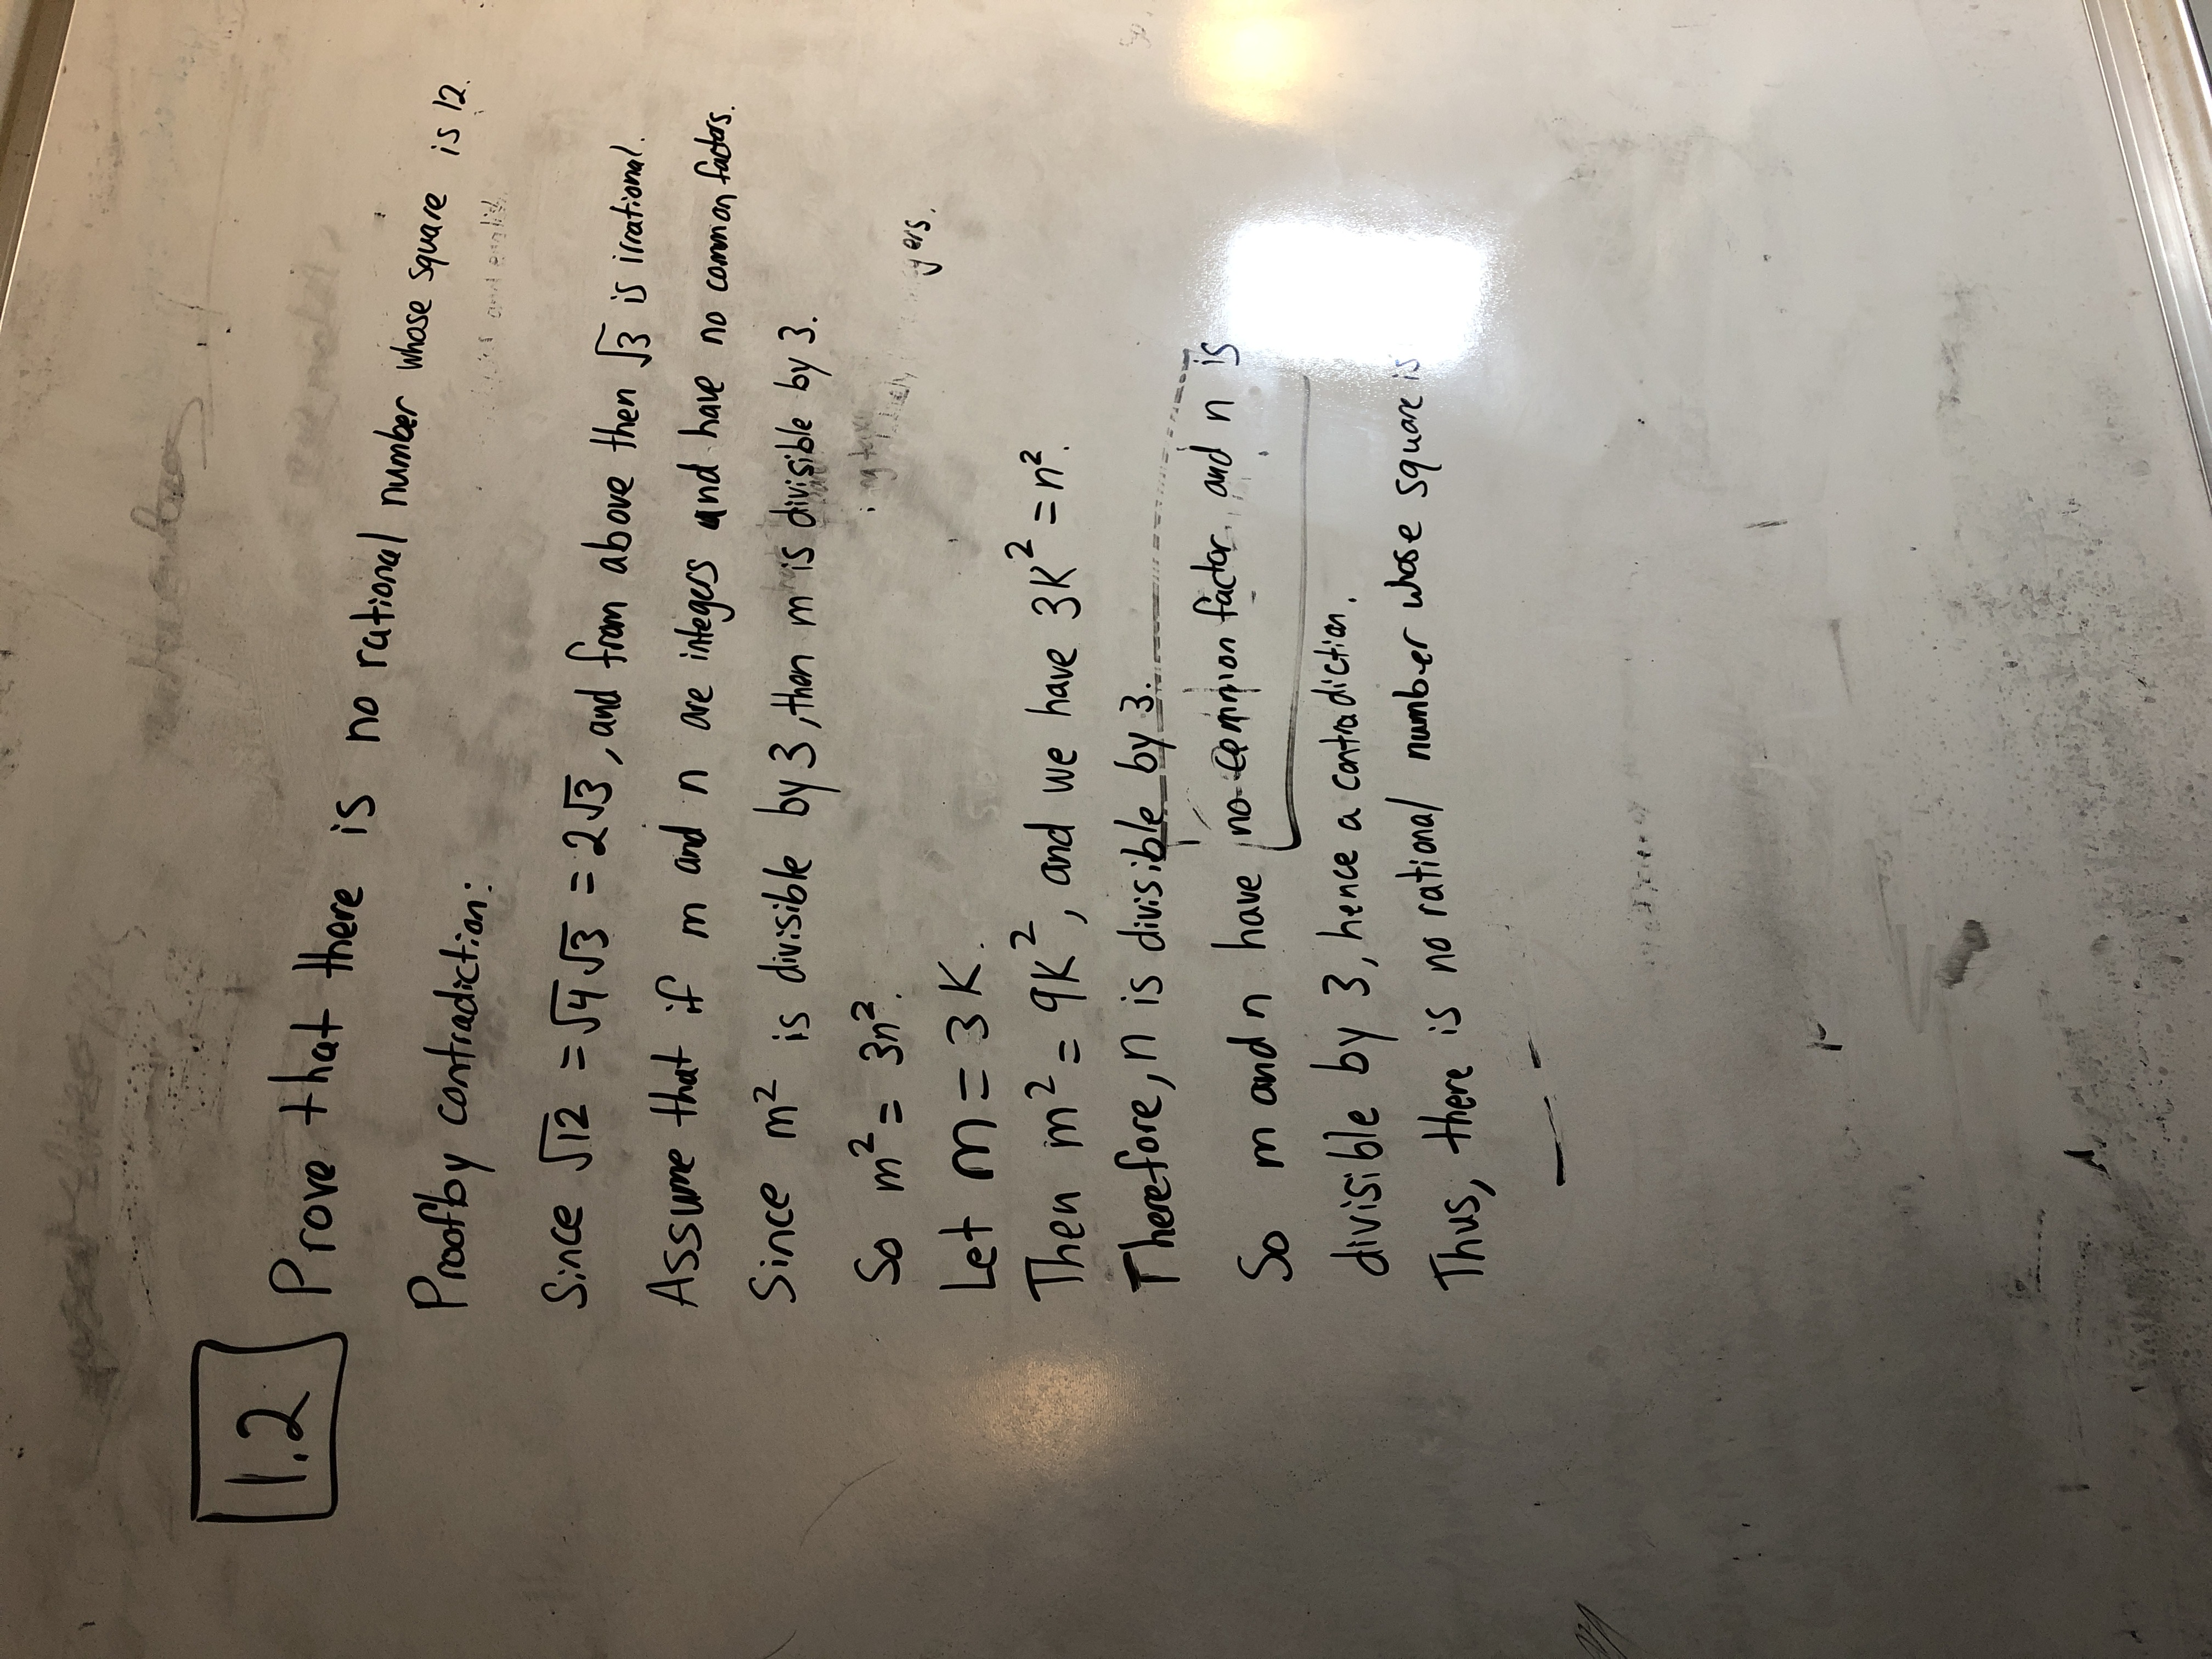
\includegraphics[angle=, origin=c,width=2.5 in]{Figures/IMG_1077.JPG}
\caption{Placeholder for my proofs} \label{fig:Euler_pic}\end{center}\end{figure} 
\newpage
\subsection{Problem 2.2}
A complex number z is said to be algebraic if there are integers $a_0, \dots, a_n,$ not all zero, such that $a_0 z^n + a_1 z^{n-1}+ \dots + a_n=0.$ \\ 
\\
Prove that the set of all algebraic numbers is countable. Hint: For every positive integer N there are only finitely many equations with $n+|a_0|+|a_1| + \dots |a_n|= N.$\\ 
\\
Proof:\\ 
Let $A_n$ be the set of integers $a_0 z^n + a_1 z^(n-1)+ \dots + a_n=0.$ \\ 
Each equation has finitely many equations that satisfy this condition. \\ 
By Theorem 2.12's Corollary, Suppose A is at most countable, and, for every $\alpha \in A, B_\alpha$is at most countable. Put T= $ \cup_{\alpha \in A}B_\alpha.$ Then T is at most countable. For T is equivalent to a subset of S=$\cup_{n=1}^\infty E_n$ then the set of algebraic numbers, $\cup_{n=2}^\infty A_N$, is at most countable. \\ 
Since the entirety of the rational numbers, Q, are algebraic, then the set of all algebraic numbers is countable. 


\begin{figure}[ht]\begin{center}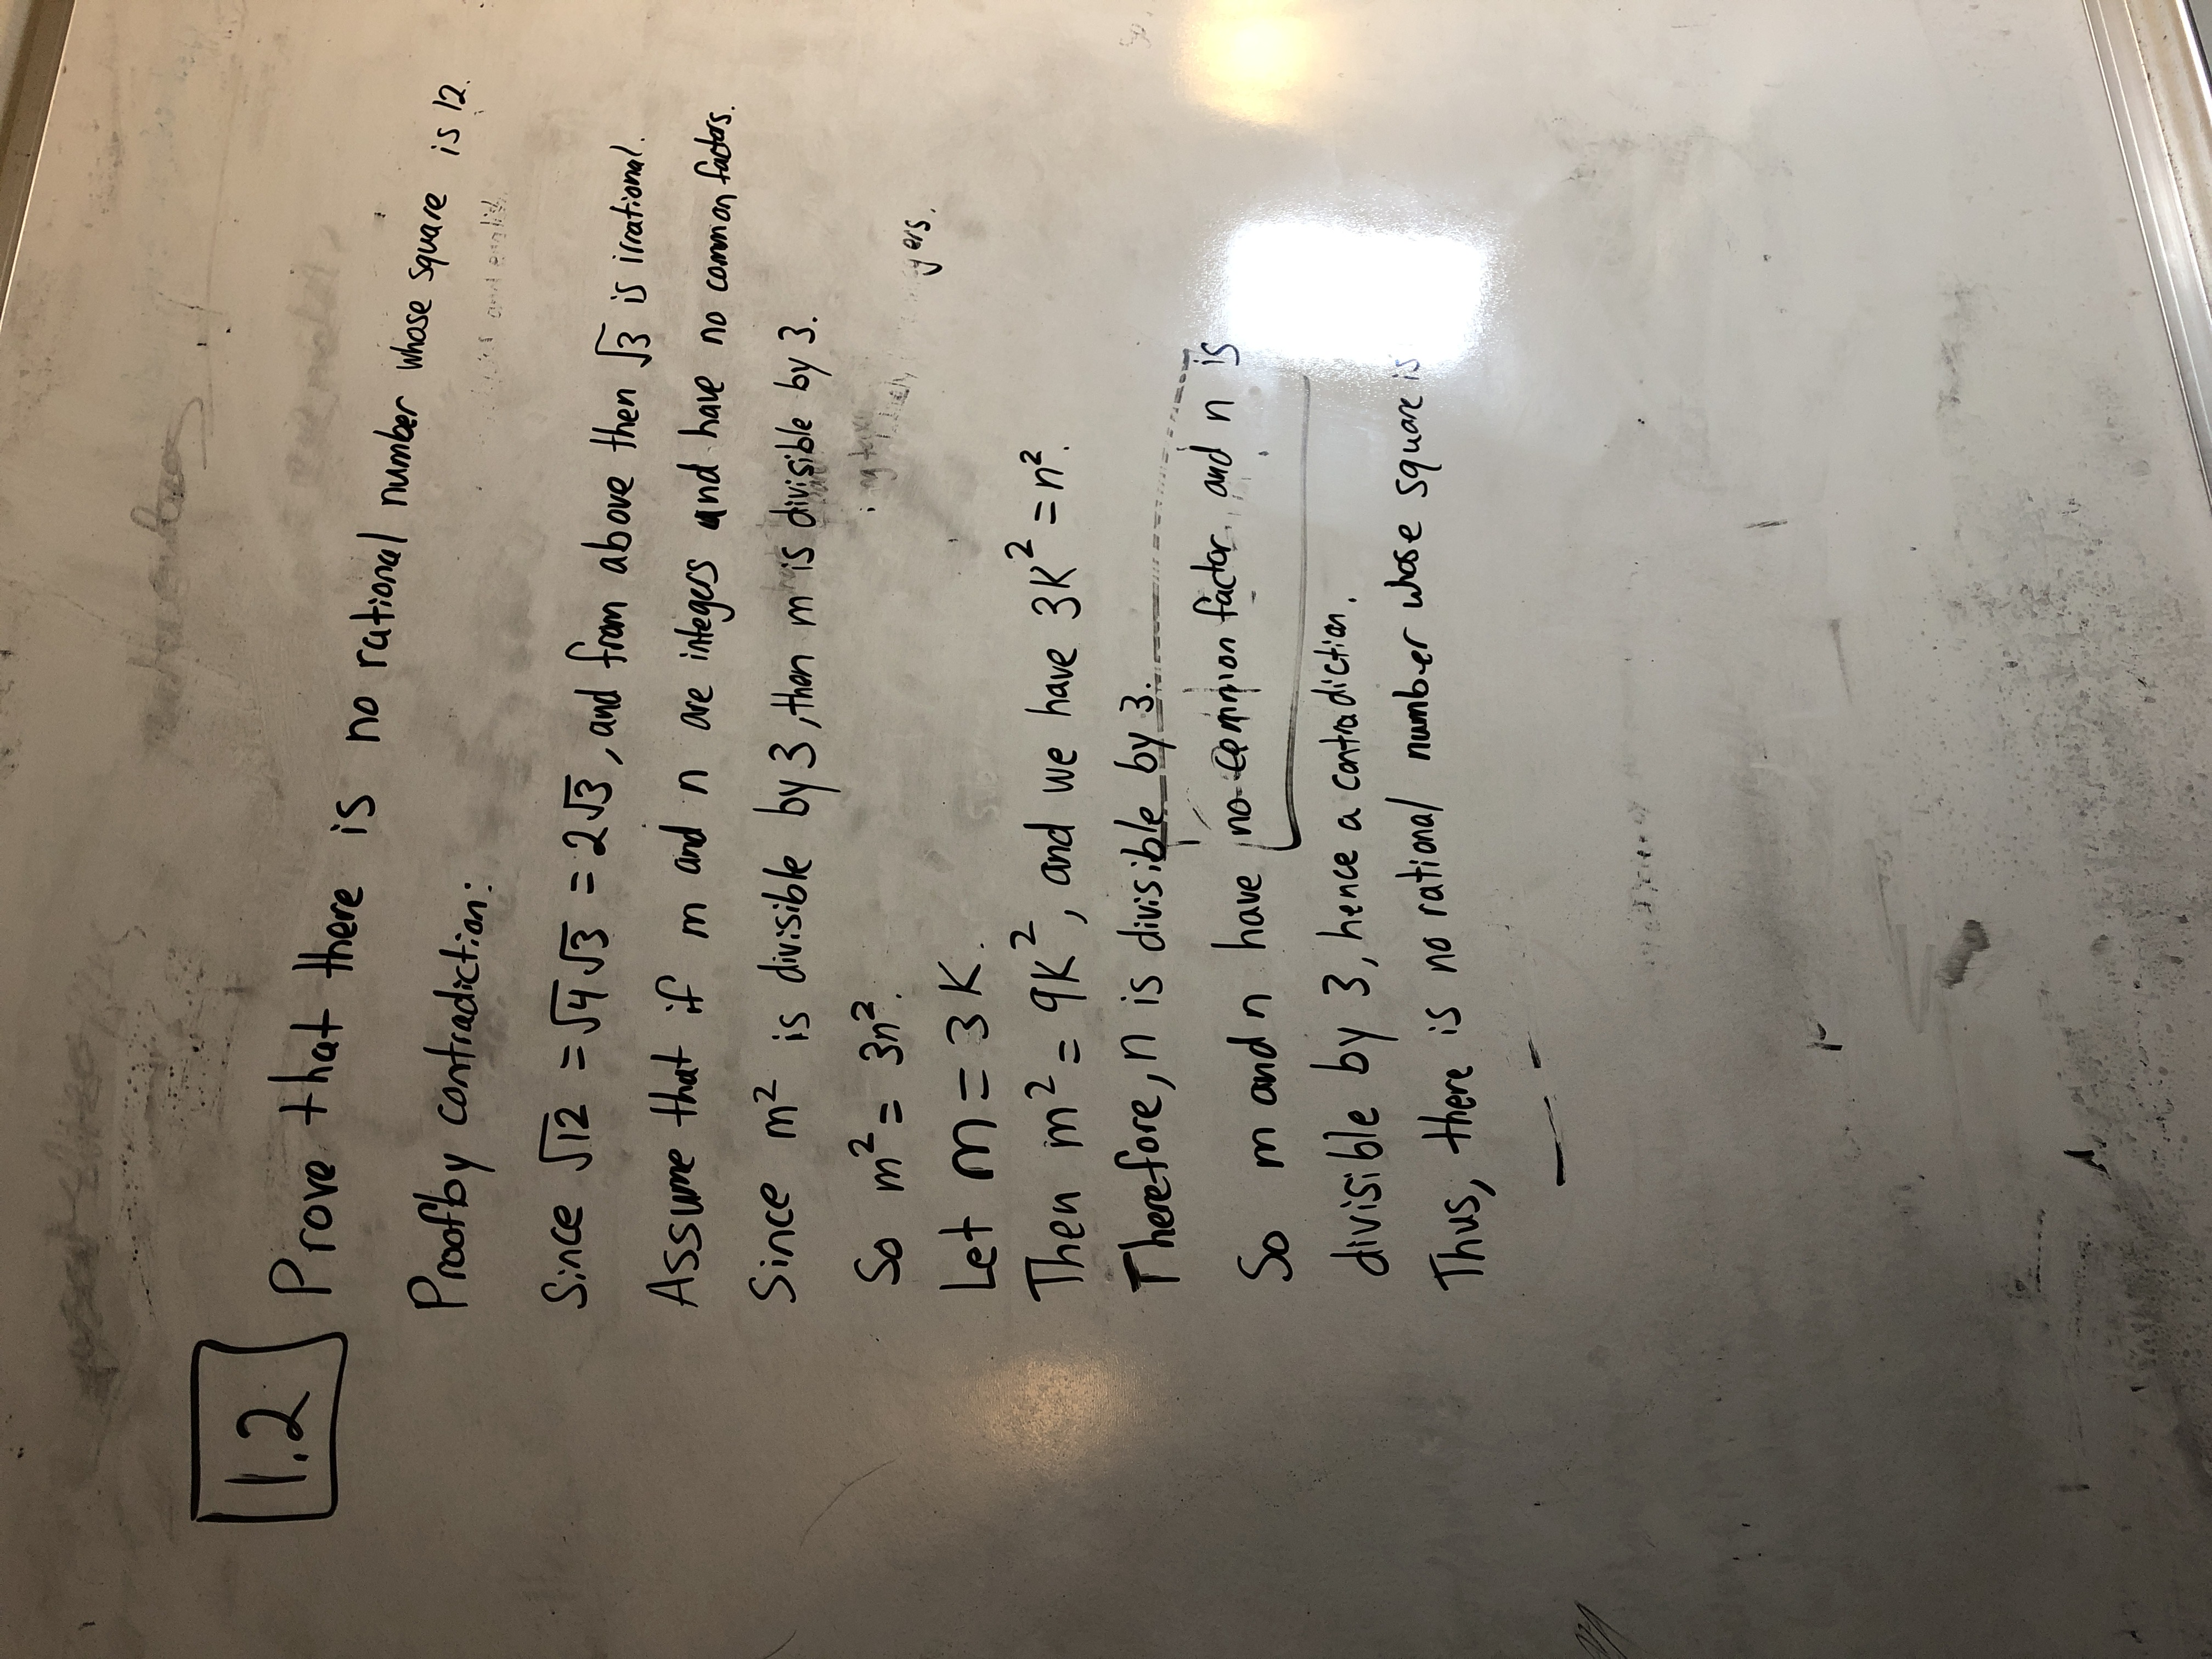
\includegraphics[angle=, origin=c,width=2.5 in]{Figures/IMG_1077.JPG}
\caption{Placeholder for my proofs} \label{fig:Euler_pic}\end{center}\end{figure} 
\subsection*{Problem 2.3}
Prove that there exist real numbers which are not algebraic. \\ 
\\
Proof:\\ 
As proved above in Problem 2.2, the set of algebraic numbers in the the set of the Real numbers is countable. \\ 
If every real number is algebraic, then the whole set of the real numbers is countable. \\
This is a contradiction, due to "the binary representation of the real numbers (base 2 instead of 10) will notice that Theorem 2.14 implies that the set of all real numbers in uncountable." \\
Thus, there exist real numbers which are not algebraic. 
\begin{figure}[ht]\begin{center}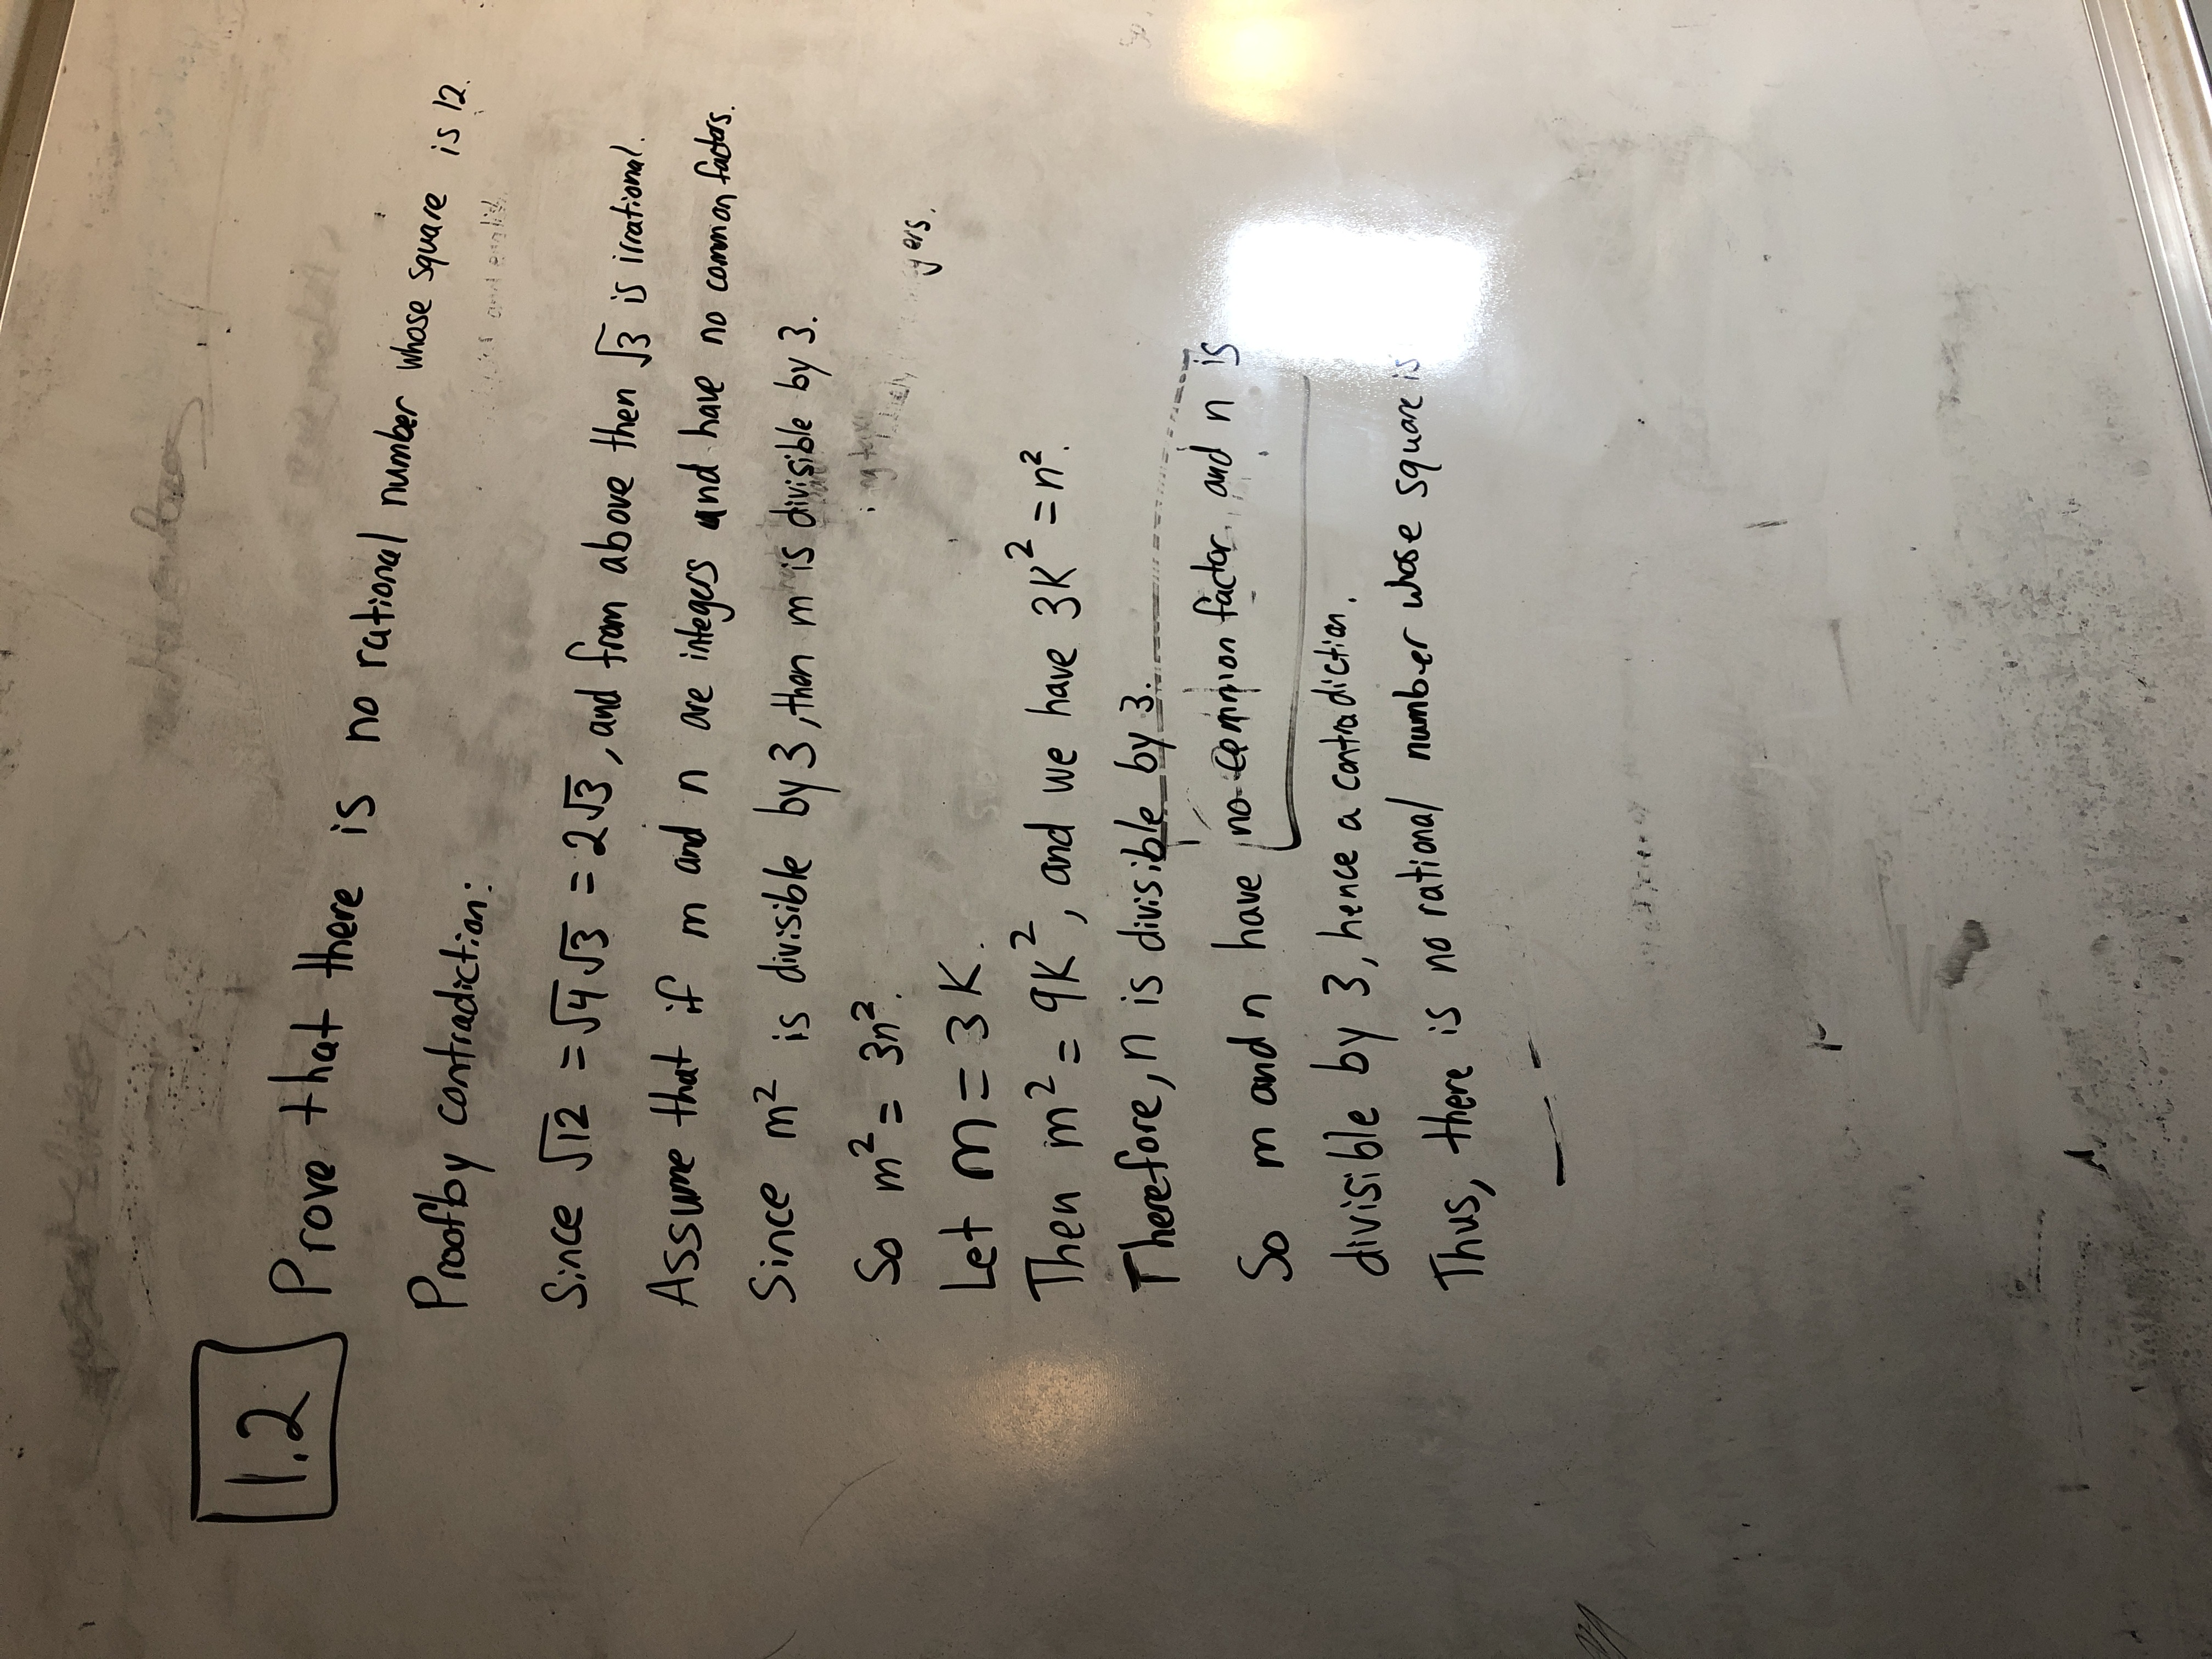
\includegraphics[angle=, origin=c,width=2.5 in]{Figures/IMG_1077.JPG}
\caption{Placeholder for my proofs} \label{fig:Euler_pic}\end{center}\end{figure} 
\\
\newpage
\subsubsection*{Problem 2.4}
Is the set of irrational real numbers countable? \\ 
No\\ 
Proof:\\ 
Since the set of real numbers, which is the union of the rational and irrational numbers, is not countable. \\ 
Thus, the set of real irrational numbers is not countable. 
\begin{figure}[ht]\begin{center}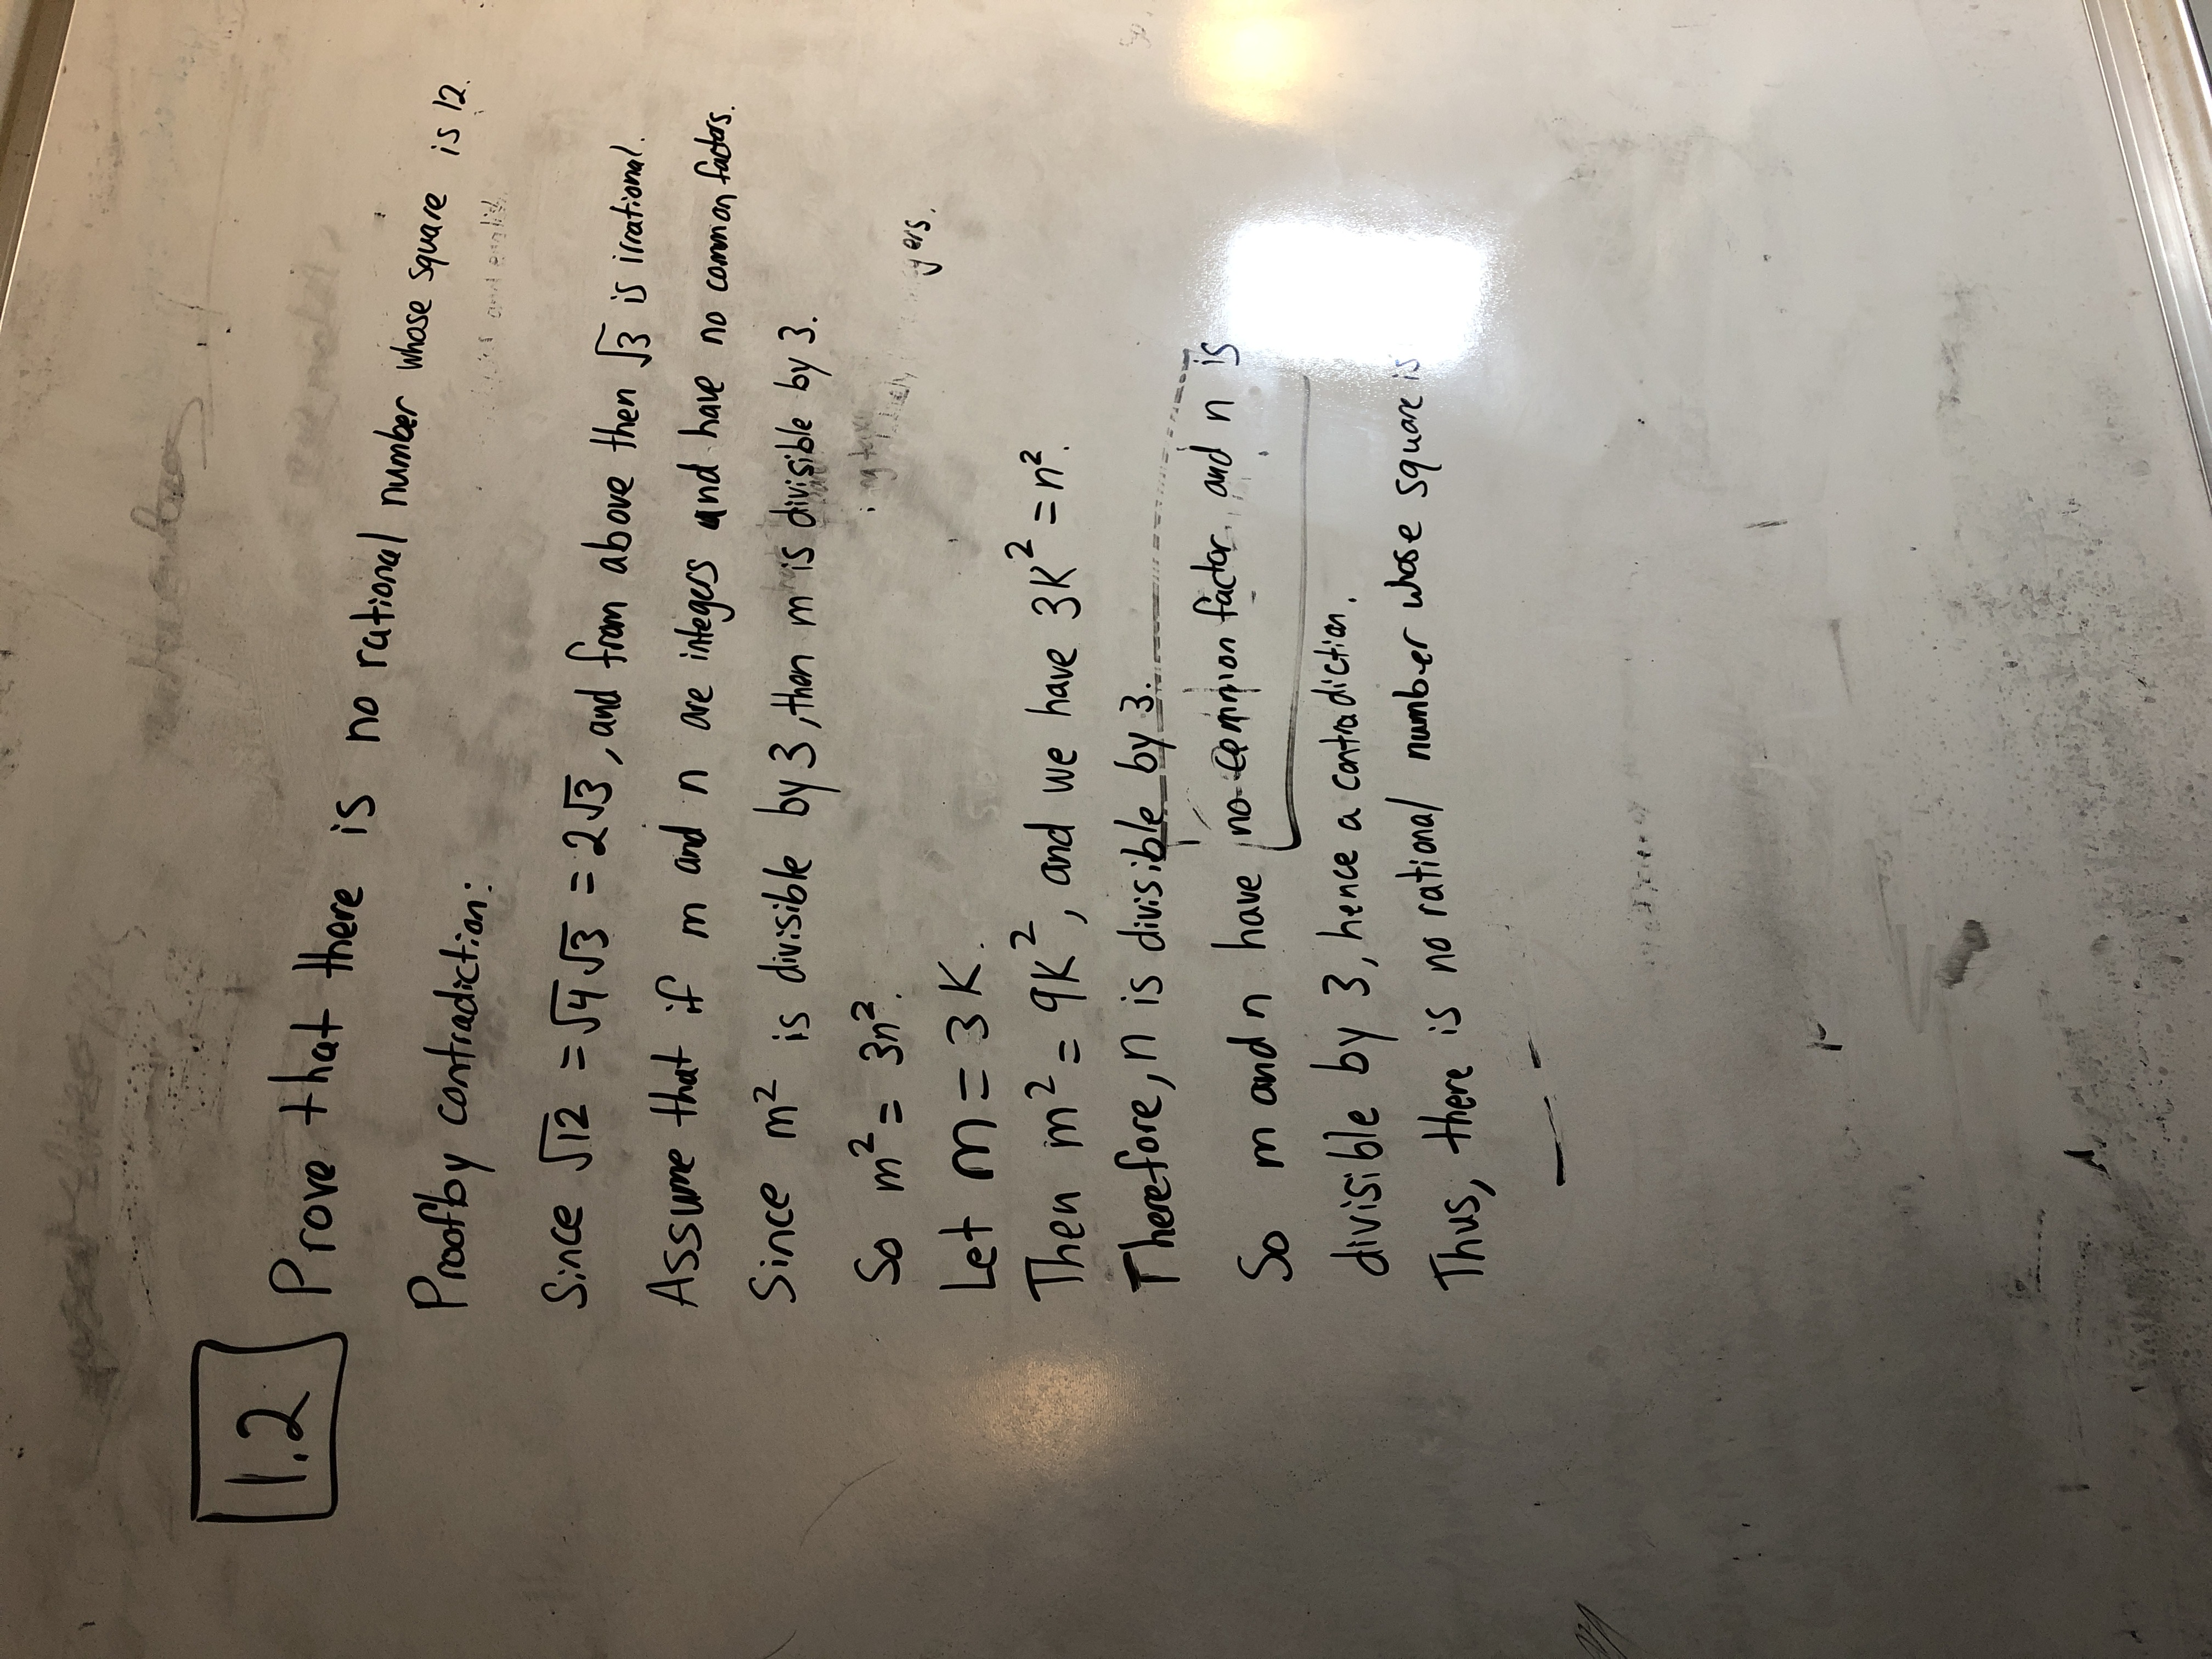
\includegraphics[angle=, origin=c,width=2.5 in]{Figures/IMG_1077.JPG}
\caption{Placeholder for my proofs} \label{fig:Euler_pic}\end{center}\end{figure} 
\\
\newpage 
\subsubsection{Problem 2.5}
Construct a bounded set of real numbers with exactly three limit points. \\
Proof:\\ 
Let E be the set of numbers in $a+ \frac{1}{n},$ where $a \in \{1,2,3\}$ and $n \in \{2,3,4,5, \dots\}.$\\
So, $\{1,2,3\} \subset E^'$, as every deleted neighborhood of 1,2, or 3 contains a point in E.\\
 Let $\delta =$ min ${|x-1|,|x-2|,|x-3|}.$\\
 If $x \notin \{1,2,3\}$, then the set U of y such that $|x-y|< \frac{\delta}{2}$ contains at most a finite number of points of E, since the set $V=(1,1+\frac{\delta}{2}) \cup (2,2+\frac{\delta}{2} \cup (3,3+\frac{\delta}{2})$ is disjoint from U, and V contains all the points of the set E except possibly the finite set of points $a + \frac{1}{n}$ for which $n \leq \frac{2}{\delta}.$ \\
 If $p_1, \dots, p_r$ are the points of E in U, let $N$ be the minimum of $\frac{\delta}{2}$ and the $|x-p_n|$ for which $x \neq p_n.$ \\
 Then the set W of points y such that $|y-x|< N$ contains no points of E except possibly x. \\
 Hence $x \in E^'.$ \\
 Thus $E^{'}=\{1,2,3\}.$


\begin{figure}[ht]\begin{center}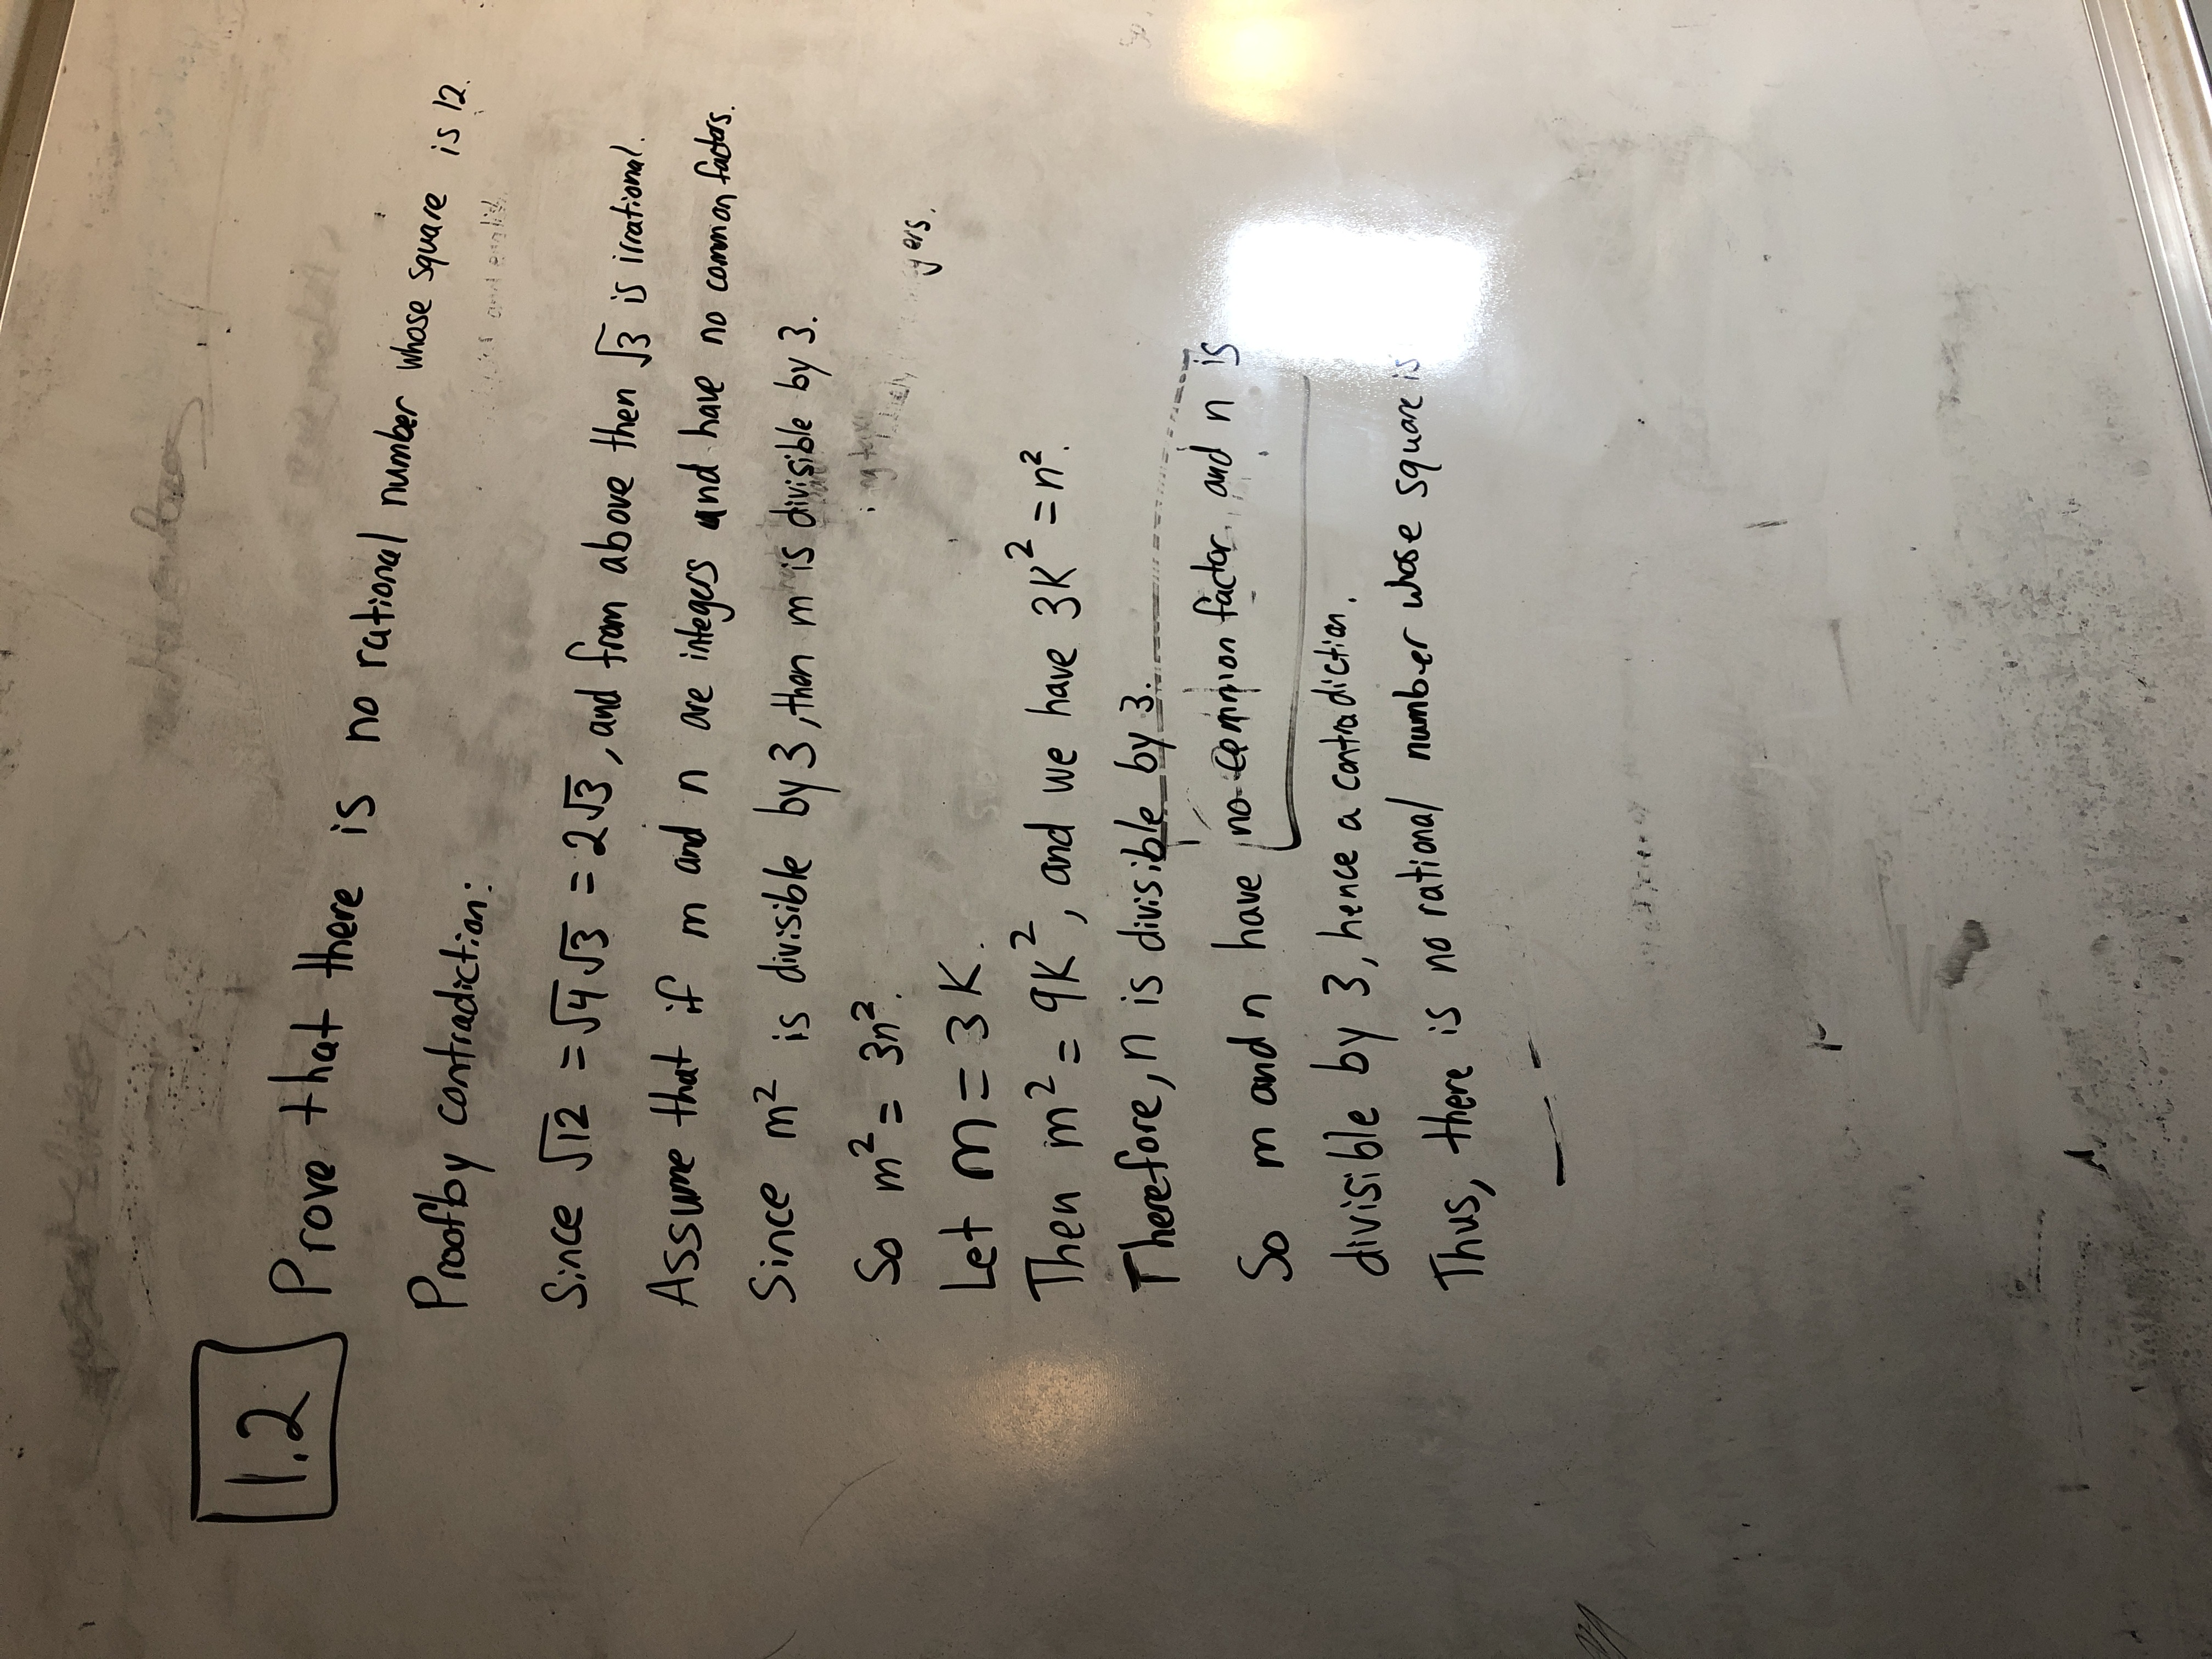
\includegraphics[angle=, origin=c,width=2.5 in]{Figures/IMG_1077.JPG}
\caption{Placeholder for my proofs} \label{fig:Euler_pic}\end{center}\end{figure} 
\\
\subsubsection{Problem 2.6}
Let $E^'$ be the set of all limit points of a set E. Prove that $E^'$ is closed. Prove that E and $\bar{E}$ have the same limit points. (Recall that $\bar{E}=E \union E^'.$) Do E and $E^'$ always have the same limit points?\\ 
Proof:\\ 
Let $x \in (\bar{E})^'.$ \\ 
Let $r>0.$\\ 
There is a point y of $\bar{E}$ such that $0<d(y,x)<r.$ \\ 
If $y \in E^',$ then z=y. \\ 
If $y \notin E$, then $y \in E^'.$ \\ 
Let $s=min(d(x,y)),r-d(x,y)),$ where $s>0.$ \\ 
Since $y \in E^',$ there exists $z \in E$ with $0<d(x,z)<s.$ \\ 
So $d(z,x) \geq d(x,y)-d(x,z)>0$ and $d(z,x) \leq d(x,y)+d(y,z)<d(x,y)+r -d(x,y)=r.$ \\ 
Next, demonstrate that E and $\bar{E}$ have the same limit points. \\ 
Suppose $x \in E^'.$ \\ 
Since every deleted neighborhood of x contains a point of E, then furthermore every deleted neighborhood of x contains a point of $\bar{E}.$ \\ 
Thus, $E^{'} \subseteq (\bar{E})^'.$ \\ 
So, E and $E^'$ may have different sets of limit points. \\ 
So one case would be if $E=\{0,1,\frac{1}{2},\frac{1}{3}, \dots, \frac{1}{n}, \dots\},$ then $E^{'}={0},$ while $(E^{'})^{'}= \emptyset.$

\begin{figure}[ht]\begin{center}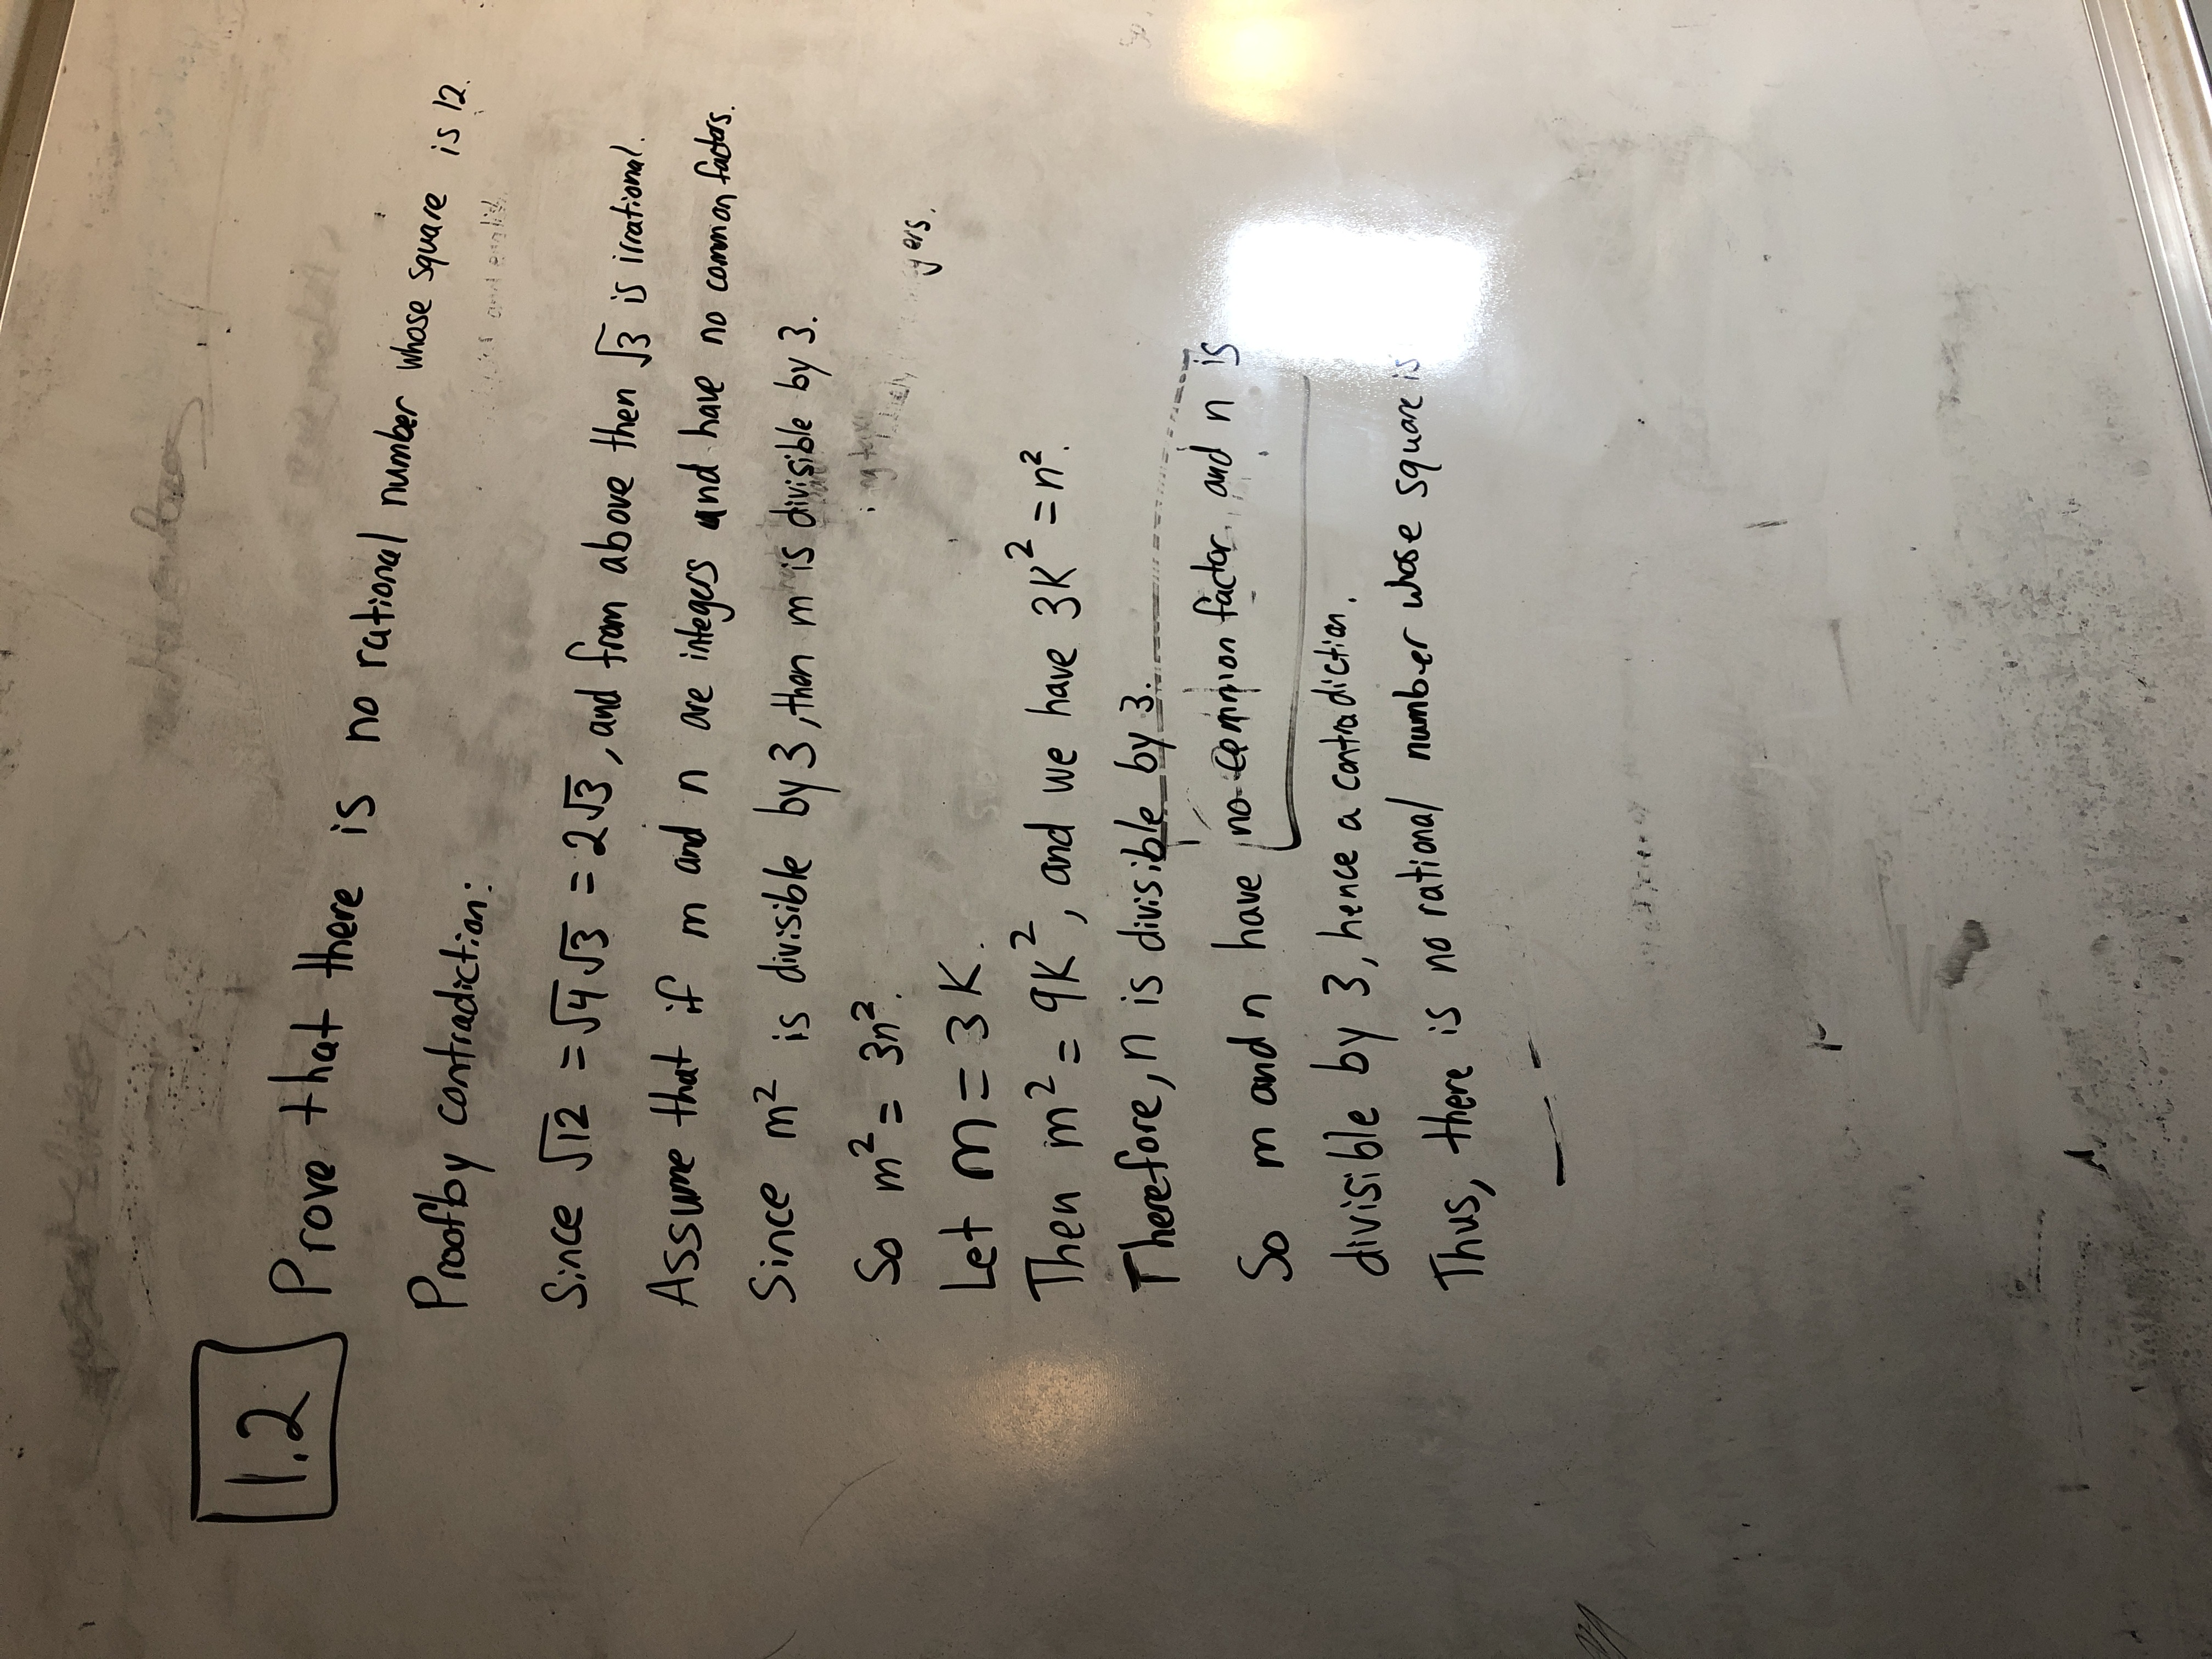
\includegraphics[angle=, origin=c,width=2.5 in]{Figures/IMG_1077.JPG}
\caption{Placeholder for my proofs} \label{fig:Euler_pic}\end{center}\end{figure} 




\subsubsection*{7}

Let $A_1, A_2, A_3, ...$ be subsets of a metric space. \\
(a)If $B_n= \cup_{i=1}^n \bar{A_i},$ for $n=1,2,3,...$ \\
Since $(E \cup F)^{'}=E^{'} \cup F^{'}$ then $\overline{(E \cup F)}=\bar{E} \cup \bar{F}.$\\ 
So if $x \in E^{'},$ then $x \in (E \cup F)^{'}.$\\
Also, if $x \in F^{'}$ then $x \in (E \cup F)^{'}.$ \\ 
By definition, $E^{'}\cup F^{'} \subseteq (E \cup F)^{'}.$ \\ 
Next, if $x \notin E^{'} \cup F^{'}.$ then there exists r>0 where the element y of E cannot satisfy $0<d(x,y)<r.$\\
Also, the same would go for s>0 where the element y of F cannot satisfy $0<d(x,y)<s.$\\
Let h= min(r,s).\\ 
It would follow that $h>0$ and the element y of the set $E \cup F$ cannot satisfy $0<d(x,y)<h.$\\
Thus, $x \notin (E \cup F)^{'}.$\\
Proof by Induction: \\ 
$\overline{B_n}=\overline{\cup_{i=1}^{n}A_i}$ \\ 
$\overline{B_n}=\overline{A_1 \cup \cup_{i=2}^{n}A_i}$ \\ 
$\overline{B_n}=\bar{A_1} \cup \overline{\cup_{i=2}^{n}A_i}$ \\ 
$\overline{B_n}=\overline{A_1} \cup \cup_{i=2}^{n}\bar{A_i}$ \\ 
$\overline{B_n}=\cup_{i=1}^{n}\bar{A_i}$ \\ 
Therefore, by induction, $\overline{B_n}=\cup_{i=1}^{n}\bar{A_i}$ for
n=1,2,3,....
\\(b)\\
Since $B \supseteq A_{i}$ for all i, then $\bar{B} \supseteq \bar{A_i}$ for all i, and so \\ 
$\bar{B} \supseteq \cup_{i=1}^{\infty}\bar{A_i}$. \\ 
Let $A_i={q_i}$ where $\{q_1, q_2,q_3, ..., q_n,...\}$ is in the set of rational numbers, then B is the full set of rational numbers. \\ 
Thus, $\bar{B}=R^{1},$ while $\bar{A_i}=A_i$ for each i, i.e. $\cup \bar{A_i}$ is the set of all rational numbers. 

\subsubsection*{8}
Is every point of every open set E $\subset R^2$ a limit point of E? Answer the same question for closed sets in $R^2.$ \\
Let E be an open set in $R^2$ let $(x_1,x_2) \in E,$ let S be such that $(y_1,y_2) \in E$ if $\sqrt{(y_1-x_1)^2 +(y_2-x_2)^2}<s$ and let $r>0.$Then the point $(z_1,z_2)=(x_1 +\frac{1}{2} min (r,s), x_2)$ belongs to E and satisfies $0<\sqrt{(z_1-x_1)^2+(z_2-x_2)^2}<r.$ 
There are closed sets for which this statement is not true. For example, any finite set E is closed, yet $E^{'}=\emptyset$ for a finite set.  
\section*{9}
Let $E^\circ$ denote the set f all interior points of a set E. [See Definition 2.18(e); $E^ \circ$ is called the interior of E.]\\ 
(a) Prove that $E^ \circ$ is always open. \\ 
(b)Prove that E is open if and only if $E^\circ =E.$ \\ 
(c)If G $\subset$ E and G is open, prove that $G \subset E^\circ.$ \\ 
(d) Prove that the complement of $E^\circ$ is the closure of the complement of E. \\ 
(e) Do E and $\bar{E}$ always have the same interiors? \\ 
(f) Do $E$ and $E^\circ$ always have the same closures? \\ 
(a) \\ 
Proof: \\ 
Let $x \in E^{\circ}.$ \\ 
Then there exists $r>0$ such that $y \in E$ if $d(x,y)<r.$ \\ 
We claim that in fact, $y \in E^0$ if d(x,y)<r, so that $x \in (E^ {\circ})^{\circ}.$ \\ 
Then if $d(z,y)<s,$ we have (by the triangle inequality) \\ d(x,z)<r, and so $z \in E.$ \\ 
By def, this means $y \in E^{\circ}.$\\ 
Since y was any point with $d(x,y)<r$, it follows that all such points are in $E^{\circ},$ and so $x \in (E^{\circ})^{\circ}.$ \\ 
(b) \\ 
Prove that E is open if and only if $E^{\circ}=E.$ \\ 
By def, E is open if and only if each of its points is an interior point, which says precisely that $E = E^{\circ}.$ \\ 
(c) If $G \subset E$ and G is open, prove that $G \subset E^{\circ}.$ \\ 
If $G \subset E$ and G is open, then $G=G^{\circ} \subseteq E^{\circ}.$ \\ 
(d)Prove that the complement of $E^{\circ}$ is the closure of the complement of E. \\ 
Part (c) shows that $E^{\circ}$ is the largest open set contained in E, i.e. the union of all open sets contained in E. \\ 
Hence its complement is the intersection of all closed sets containing the complement of E, and this, by theorem 2.27 (c), is the closure of the complement of E. \\ 
(e) Do E and $\bar{E}$ always have the same interiors? \\ 
No. \\ 
If E is the rational numbers in the space $R^{1},$ then \\ 
$E^{\circ}=\emptyset,$ while $\bar{E}=R^1,$ so that the interior of $\bar{E}$ is $R^1.$ \\ 
(f) Do E and $E^{\circ}$ always have the same closures? \\ 
No. If E is the rational numbers in the space $R^{1},$ then $\bar{E}=R^{1}$, while $E^{\circ}=\emptyset,$ so that $\bar{E^{\circ}}=\emptyset.$\\ 
\subsubsection*{11}
For $x \in R^1$ and $y \in R^1,$ define \\ 
$d_1(x,y)=(x-y)^2$ \\ 
$d_2(x,y)=\sqrt{|x-y|}$\\ 
$d_3(x,y)=|x^2-y^2|$\\ 
$d_4(x,y)=|x-2y|$ \\ 
$d_5(x,y)= \frac{|x-y|}{1+|x-y|}$\\ 
Determine, for each of these, whether it is a metric or not. \\
The function $d_{1}(x,y)$ fails the triangle inequality condition, since $d_{1}(0,1)+d_{1}(1,2)=1+1=2<4=d_{1}(0,2).$\\ 
The function $d_2(x,y)$ meets the triangle inequality condtion, since $|x-z|\leq \sqrt{|x-y|}+\sqrt{|y-z|}$, as one can easily see by squaring both sides. Hence $d_2$ is a metric. \\ 
The function $d_{3}(x,y)$ fails the positivity condition, since $d_{2}(1,-1)=0.$ \\
(Restricted to $[0, \infity]$, $d_{3}$ would be a metric.) \\ 
Since $d_{4}(1, \frac{1}{2}=0,$ the function $d_{4}(x,y)$ likewise fails the positivity condition. It also fails the symmetry condition, since $d_{4}(x,y)$ likewise fails the positivity condition. It also fails the symmetry condition, since $d_{4}(x,y) \neq d_{4}(y,x)$ in general. \\ 
The function $d_{5}(x,y)$ is a metic. 
In fact we can prove more generally that if d(x,y) is a metric, so is $p(x,y)= \frac{d(x,y)}{1+d(x,y)}$. It is obvious that p meets the nonegativity and symmetry requirements and we need only verify the triangle inequality, 
which in this case says that \\ 
$\frac{d(x,z)}{1+d(x,z)} \leq \frac{d(x,y)}{1+d(x,y)}+\frac{d(y,z)}{1+d(y,z)}.$\\ 
To do this, let a=d(x,z), b=d(x,y) and c=d(y,z). We need to show that if $a \leq b+c,$ then \\ 
$\frac{a}{1+a}\leq \frac{b}{1+b}+\frac{c}{1+c}.$\\ 
Clearing out the denominators, we find this inequality to be equivalent to $a+ab+ac+abc \leq b+c+ab+ac+2bc+2abc,$ which is clearly true. \\ 
\subsubsection*{12}
Let $K \subset R^1$ consist of 0 and the numbers $1/n$, for $n=1,2,3,...$ Prove that k is compact directly from the definition (without using the Heine-Borel theorem.)\\ 
Suppose $K \subset U_{\alpha}$ is open. \\ 
Then 0 must be in some set $U_{\alpha 0}.$\\ 
Since $U_{\alpha 0}$ is open, there exists $\delta >0$ such that $(- \delta , \delta) \subset U_{\alpha 0}.$\\ 
In particular $\frac{1}{n} \in U_{\alpha 0}$ if $n> \frac{1}{\delta}.$ \\ 
Let N be the largest integer in $\frac{1}{\delta},$ and let $\alpha_j, j=1,...,N,$ be such that $\frac{1}{j} \in U_{\alpha j}.$\\ 
Then $K \subset \cup_{j=0}^N U_{\alpha j}.$
\subsubsection*{13}
Construct a compact set of real numbers whose limit points form a countable set. \\ 
Let $E={0} \cup {\frac{1}{n}: n \in N}.$ $E \subset [0,1],$ the only limit point of E is 0, and $0 \in E,$ so E contains all of its limit points. It is thus closed and bounded, and therefore it it compact. \\ 
Let $K_{n}=2^{-n}.$ \\ 
$E +\sum_{k=0}^{n-1} 2^{-k}$ and $k=(\cup_{n=0}^\infinity K_n)\cup {2}.$\\ 
The only limit point of $k_n$ is $\sum_{k=2}^{n-1}2^{-k}.$\\ 
Thus, k has countably many limit points in $[0,2),$ and they are given by ${0} \cup {2-2^{-n}}_{n=0}^{\infty} k.$ has no limit points in $(\-\infity,0)$ and none in $(2, \infty)$.\\ 
2 is a limit point of k because 2= $lim_{n \longrightarrow \infty} 2-2^{-n},$ but $2 \in k. $\\ 
Thus, k contains its $\subset R$ limit points, and so it is closed. k $\subset [0,2],$ so k is bounded. Hence k is a compact set with countably many limit points.
\subsubsection*{14}
Give an example of an open cover of the segment (0,1) which has no finite subcover. \\ 
Consider ${A_j}_{j=1}^{\infity}$ where $A_j=(2^{-j},1).$\\ 
To prove ${A_j}$ is an open cover, let $x \in (0,1).$\\ 
If we choose j large enough so that $2^{j}>x^{-1},$ then $2^{-j}<x<1,$ and so $x \in A_j.$ To prove that there is no finite subcover, let ${A_{nk k=1}}^{m}$ is a finite subset of ${A_j}.$\\ Let $N=max_{1} \leq k \leq m \cap_{k}.$\\
Since $A_1 \subset A_2 \subset ..., \cup_{k=1}^m A_{nk}=A_N.$\\ 
For $x \in (0,2^{-N}),x \notin A_N,$ and so ${A_N}^m$, is not an open cover of $(0,1).$ Thus, ${A_j}$ has no finite subcover.  

\subsubsection*{15}
Show that Theorem 2.36 and its Corollary become false (in $R^1$, for example) if the word "compact" is replaced by "closed" or by "bounded."\\ 
Theorem 2.36 says that if ${k_\alpha}$ are compact and if $\cap_{\alpha \in A}K_{\alpha}=\emptyset$ whenever $|A|<\infty,$ then $\cap_{\alpha}K_{\alpha} \neq \emptyset.$ \\ 
Its corollary states that if ${k_n}$ are compact and $k_1 \supset k_2 \supset ...,$ then $\cap_{1}^\infty k_n= \neq \emptyset.$ Any counterexample to the corollary is also one for the theorem. \\ 
Closed: Let $k_n=[n, \infty).$ Then $k_{n+1} \subset k_n \forall_n.$\\ 
$\forall_x \in R, $there exists $n \in N$ such that $n>x$, so $x \in K_n$ $\supset \cap_{i=1}^\infty,$ so $\cap_{1}^{\infty} k_i=\emptyset.$\\ 
Bounded: Let $k_n=(0,\frac{1}{n}].$ Then $k_{n+1}=(0,\frac{1}{k+1}] \subset (0, \frac{1}{n}]=k_n \forall n.$\\ 
Thus, $\cap_{1}^\infty k_i=\emptyset.$\\ 
Let $x \in R.$\\ 
If $ x \leq 0$ or $x \geq 1,$ then $x \notin k_1 \supset \cap_{1}^{\infty}k_i.$\\ 
If $x \in (0,1),$ then there exists $n$ such that $\frac{1}{n}<x,$ so $x \notin (0, \frac{1}{n}]= k_n \supset \cap_1^\infty.$


16, 17, 19, 22, and 29 
\subsubsection*{16}
Regard Q, the set of all rational numbers, as a metric space, with $d(p,q)=|p-q|.$ Let E be the set of all $p \in Q$ such that $2<p^2<3.$ Show that E is closed and bounded in Q, but that E is not compact. Is E open in Q? \\
Let $E= [(-\sqrt{3},-\sqrt{2})\cup (\sqrt{2}, \sqrt{3})] \cap Q$, where Q is the set of rational numbers. \\ 
For E to be bounded in Q, $M \in R$ where R is the set of the real numbers and $q \in Q$ such that $|p-q|<M$ for all $p \in E$ would have to be true. \\ 
So let $q=0$ and $M=\sqrt{3}$ since for all $p \in E,$ $|p|<\sqrt{3}=M.$\\ 
Then for E to be closed, let $p \in Q$ where Q is the set of rational numbers, be a limit point of E. \\ 
By definition, every neighborhood of p contains some q=p such that $q \in E.$\\ 
Assume $p \notin E.$\\ 
Since $p \notin Q,$ then $p \in (\infty, -\sqrt{3}) \cup (-\sqrt{2}, \sqrt{2}) \cup (\sqrt{3}, \infty).$ \\ 
Let F be a union of three disjoint open intervals. \\ 
Then p belongs to one of these three disjoint sets. \\ 
So there exists an open neighborhood I of p such that $p \in I \subset F \subset E^{c}.$\\ 
Hence a contradiction, that p is a limit point of E. \\
Thus, $p \in E.$\\ 
So E contains its limit points and this is closed. \\ 
E is not compact: \\ 
Let $x_{0}=\sqrt{2}<x_1<x_2<x_3<...<x_n$ where $x_n \in \frac{R}{Q}$ and $x_n<\sqrt{3}$ for all n, and $lim_{n \longrightarrow \infty} x_n = \sqrt{3}.$ Let $U = u \cup {u_i}$ where $u=(-\sqrt{3},-\sqrt{2}) \cap Q$ and $U_i=(x_{i-1},x_i) \cap Q $ for all i $\in N.$ U is an open cover of E. \\ 
So each set in U is open. \\ 
Then, all sets in u are disjoint so if U is an open cover, then there cannot be a finite subcover. \\ 
So let $x \in E.$\\ 
If $x<0, x\in U.$\\ 
Otherwise, since $x \in Q, x \neq x_i$ for any i. \\ 
Thus, there exists i such that $x_{i-1}< x< x_{i}.$ so $x \in U_i.$\\ 
So $x \in U_i.$\\ 
Then U covers E. \\ 
Thus, E is not compact.\\ 
E is open in Q: \\ 
$\cup {v \in U} \supset E,$ and since for all $ V \in U$ then $v \subset E,$ $\cup{v \in U}\subset E,$\\ 
So, $E= \cup{V\in U}$ is open. 


\subsubsection*{17}
Let E be the set of all $x \in [0,1]$ whose decimal expansion contains only the digits 4 and 7. Is E countable? Is E dense in [0,1]? Is E compact? Is E perfect? \\ 
Is E countable: \\ 
No. \\ 
For any list of the elements $\{a_1,a_2,,...,a_n\}$, there can always be an element a of the set E that is not in this list. \\ 
This can be done by the nth digit of a is 4 if the nth digit of $a_n$ is 7 and equal to 7 if the nth digit of $a_n$ is 4.  Is E dense in $[0,1]?$\\ 
No, since $E \subset[0.4,0.8].$\\ 
Is E compact? \\ 
Yes. \\ 
E is closed:\\ 
Let $x \in [0,1]|E,$ the decimal expansion of x contains a digit that is not 4 and 7. \\ 
Let the first digit be in the nth place $(x_n).$\\ 
Let y be any element of E. \\ 
Let the first digit where x and y have a difference of the mth digit where $(m \leq n,x_m \neq y_m).$\\ 
Then $|x-y|\geq 10^{-m}- \epsilon.$\\ 
$\epsilon \leq \sum_{k=m+1}^\infty 10^{-k}|x_k-y_k|.$\\ 
Since $y_k \in \{4,7\}$ and $x_k \in \{0,1,2,3,4,5,6,7,8,9\}.$\\ 
So, $|x_k-y_k|\leq 7.$\\ 
Thus, $\epsilon \leq \frac{7}{9}10^{-m}.$\\ 
Then, $|x-y|\geq \frac{2}{9 \cdot 10^m}\geq \frac{1}{9 \cdot 10^n.}$\\ 
So, x is an interior point of $[0,1]|E.$\\ 
Thus, E is closed. \\ 
Therefore E is closed an bounded. \\ 
Hence, E is compact. \\ 
E is perfect. \\ 
Let $x \in E$ and each $ \epsilon >0$ there is a point $y \in E$ with $0<|x-y|<\epsilon$ by setting the nth digit of x from 4 to 7 or from 7 to 4 in the nth place for any $n>1-log_{10} \epsilon.$\\ 
Then $x \in E^{'} E \subseteq E^{'}.$\\ Since we proved above that E is closed then $E=E^{'}.$ \\ 
Thus, E is perfect. 
\subsubsection*{19}
(a) If A and B are disjoint closed sets in some metric space , prove that they are separated. \\ 
(b) Prove the same for disjoint open sets. \\ 
(c) Fix $p \in , \delta >0,$ define A to be the set of all $q \in $ for which $d(p,q)< \delta,$ define B similarly, with $>$ in place of $<.$ Prove that A and B are separated. \\ 
(d) Prove that every connected metric space with at least two points is uncountable. Hint: Use(c)\\ 
(a) $A \cap B = \emptyset.$ \\ 
Since A and B are closed then $A \cap \Bar{B}=\emptyset=\Bar{A} \cap B.$\\ 
Then A and B are separated. \\ 
(b)Since $x |B$ is a closed set that contains A then by theorem 2.27 (c) $X | B \supseteq \Bar{A}.$\\ 
So, $\Bar{A} \cap B= \emptyset.$ \\ 
Also, $A \cap \Bar{B}= \emptyset.$\\ 
(c) Due to the fact that sets A and B are disjoint open sets, then by (b) above they are also separated. \\ 
(d)Let $x \in X$ and $y \in X.$\\ 
Let $ d(x,y)=d>0.$\\ 
Then for every $\delta \in (0,d),$ there must be a point z such that $d(x,z)=\delta.$\\ 
Thus, there exists a subset of X that can be placed in one-to-one correspondence with the interval [0,d], and so X is uncountable. 
\subsubsection*{22}
A metric space is called separable if it contains a countable dense subset. Show that $R^k$ is separable. Hint: Consider the set of points which have only rational coordinates. \\ 
$Q^k$ is a direct product of finitely many countable sets. \\ 
Thus, it is countable. \\ 
$Q^k \subset R^k.$\\ 
For it to be a countably dense subset: \\ 
Let U be and open subset of $R^k.$\\ 
U contains an open ball $B=B_r(x).$\\ 
B contains an open rectangle $R= \Pi_{i=1}^k(a_i,b_i).$\\ 
Then , for all i, there exists $c_i \in Q \cap(a_i,b_i).$\\ 
So $c=(c_1,...,c_k)\in Q^k \cap R \subset Q^k \cap U.$ \\ 
Thus, $Q^k$ is a dense set. \\ 
Therefore, $Q^k$ is a countable dense subset of $R^k.$ \\
This follows directly that $R^k$ is separable. 
\subsubsection*{29}
Prove that every open set in $R^1$ is the union of an at most countable collection of disjoint segments. Hint: Use Exercise 22. \\ 
Let O be open. \\ 
For each pair of points $x \in O$ and $y \in O$ the equivalence relation is $ x ~ y iff [min(x,y),max(x,y)] \subset O.$\\ 
This is an equivalence relation.
Reflexive: \\ 
$[x,x] \subset O$ if $x \in O$
So, $x ~ x$. \\ 
Symmetric: \\ 
$min(x,y)= min(y,y)$ and $max(x,y)=max(y,x)$\\
So, $x~y and y ~x.$\\ 
Transitive: \\ 
$[min(x,z),max(x,z)] \subseteq [min(x,y),max(x,y)] \cup [min(y,z),max(y,z)] \subseteq O.$ \\ 
So $x~y$ and $y~z,$ then $x~z.$\\ 
Then, $min(x,z)\geq min(min(x,y),min(y,z))$ and $max(x,z)\leq max(max(x,y),max(y,z)).$\\ 
O can be written as a disjoint union of pairwise disjoint equivalence classes. \\ 
Let each equivalence class be an open interval. \\ 
For each $x \in O,$ let $A=\{z:[z,x]\subseteq O\}$ and B=$\{z:[x,z] \subseteq O.$ \\ 
Let $a= infA$ and $b=supB.$\\
So $(a,b) \subset O.$\\ 
If $a<z<b,$ there exists $c \in A$ where $c<z$ and $d \in B$ with $d>z.$ \\ 
Then $z \in [c,x] \cup [x,d] \subseteq O.$ \\ 
So, (a,b) is the equivalence class that contains x. \\ 
Each element of (a,b) is equivalent to x. \\ 
Suppose $z<a.$\\
If z was equivalent to x then $[z,x]$ would be contained in O. \\ 
So, $z \in A.$ \\ 
Thus, a wouldn't be a lower bound for A. \\
Also, if $z>b$ and $z~x,$ then b could not be an upper bound for B. \\ 
Therefore, $z \notin (a,b).$\\ 
Since O is a union of pairwise disjoint open intervals then it most be at most countable. \\ 
This is due to the fact since each open interval contains a rational number that is not in any other interval. \\ 
Hence, every open set in $R^1$ is the union of an at most countable collection of disjoint segments. 




\newpage
\section{The Second Compilation}
\section*{Me Pontificating}
Here is me being a control freak and doing all the work now so I can return to my simulations and practice numerical relativity projects with CCRG as planned. Thank you for your understanding. I do need an A in this course as the fellowships, scholarships, grants, programs, and institutions I am interested in do indeed care about my final gpa. Please provide any feedback for these cases. \\ 

\section*{Dr.O'Shaugnessy why is it cool and relates to my research?: Independent Study and engagement idea to have me not go rogue and research and study optics and fourier analysis and tensors and question why I'm classified as a math major at this institution}

\section{Cesaro Summable Question }

\subsection{The Problem itself}


\subsection{Relevant readings}

\subsection{Me pontificating}


\subsection{Proofs and work}


\section{Newton's method}

\subsection{The Problem itself}
(25 pts) Newton's method for estimating the real cube root of a positive real number Z is to start with an arbitrary guess, $x_0,$ and to generate an infinite sequence ${x_n}$ recursively with the recursion relation \\ 
$x_{n+1}=\frac{2}{3}x_{n}+\frac{1}{3}\frac{z}{x_n^2}$\\ 

Prove that if $x_0 > 0, $ then as long as none of the iterates equals zero the sequence ${x_n}$ converges to the cube root of Z. There are some negative values of $x_0$ for which the sequence ${x_n}$ does not converge, values for which the recursion formula that defines the sequence produces an undefined term because of a would-be division by 0 after a finite number of terms. Characterize those negative values of $x_0$ and prove that for all other negative values of $x_0$ the sequence ${x_n}$ converges to the cube root of Z.

\subsection{Me pontificating}

\subsection{Proofs and work }


\section{Convergence series}


\subsection{Me Pontificating}
Why would I care? My research is based on Bayesian statistics converging methods. I mean this is the simplistic look at the idea...but the exercise has merit and I should be looking at O3 and O4.  
\subsection{The problem itself}
(25 Points) \\ 
Let $b_n=$ \[ \begin{cases} 
      1 & 2^{2k}\leq n <2^{2k+1} \\
      -1 & 2^{2k+1} \leq n\leq 2^{2k+2} 
   \end{cases}
\] 
for K=0,1,2,... \\ 
Determine whether the series $\sum_{n=2}^\infty \frac{b_n}{n log(n)}$ converges. Prove your claim. (9 points). \\ 
\begin{figure}[h]\begin{center}\includegraphics[angle=, origin=c,width=2 in]{WhiteboardPictures/Exam 2/IMG_1052.JPG}
\caption{Placeholder for my proofs} \label{fig:Euler_pic}\end{center}\end{figure} 

\newpage
Determine whether the series $\sum_{n=2}^\infty \frac{b_n}{n}$ converges. Prove your claim. (8 points). \\ 
\begin{figure}[h]\begin{center}\includegraphics[angle=, origin=c,width=2 in]{WhiteboardPictures/Exam 2/IMG_1052.JPG}
\caption{Placeholder for my proofs} \label{fig:Euler_pic}\end{center}\end{figure} 

\newpage 
Determine whether the series $\sum_{n=2}^\infty \frac{b_n}{n^2}$ converges. Prove your claim. (8 points). \\ 

\begin{figure}[h]\begin{center}\includegraphics[angle=, origin=c,width=2 in]{WhiteboardPictures/Exam 2/IMG_1052.JPG}
\caption{Placeholder for my proofs} \label{fig:Euler_pic}\end{center}\end{figure} 

\newpage


\section{Bifurcation Diagram}


\subsection{Me Pontificating about why I care about chaos dynamics}
This is rudimentary newton's method and the time complexity is baseline. Here is where I talk about the wikipedia article I read a while ago and going to talk about it again. 


\subsection{The Problem Itself}
(25 points total) In a seminal paper May [1] presented and analyzed simple difference equation
models of biological systems that have chaotic dynamics. May and other researchers in this field
emphasize, as a typical example, the logistic model as expressed in this recurrence formula: \\ 
$x_{N+1}=rX_N(1-X_N)$ \\ 
Here, $X_N$ is a population at the Nth time period after the initial time period. (See[1] and particularly [3] for examples). The parameter r is fixed. We start with an initial population— $x_0$
 —
and the formula lets us compute the population at successive time periods. (The Wikipedia article
on this topic [2] is worth reading.) The recurrence formula produces an infinite sequence that
characterizes the evolution of the population; that sequence depends on r and $x_0$
.
For the formulation given by our recurrence relation, r is positive and $0 < x_0 < 1$.
This model is associated with an interesting and famous bifurcation diagram: \\ 


You should read the Wikipedia article [2] for a thorough account of this diagram; I am just going to
summarize the bits that are important for this problem. For values of r between 2 and 3, the
sequence produced by the recurrence formula converges, and for a fixed r all of the sequences,
regardless of $x_0$
 , converge to the same value. This is why there is a single point on each line r = constant between 2 and 3 on the bifurcation diagram. For values of r between 3 and about 3.45,
the sequence produced by the recurrence formula does not converge, but asymptotically its
elements oscillate between two values, and for a fixed r all of the sequences—with one
exception--regardless of $x_0$
 , oscillate asymptotically between the two values. This is why there
are two points on each line r = constant between 3 and about 3.45, on the bifurcation diagram.
For values of r between about 3.45 and about 3.54, the sequence produced by the recurrence
formula does not converge, but asymptotically its elements oscillate among four values, and for a
fixed r all of the sequences—with a few exceptions--regardless of $x_0$
 , oscillate asymptotically
among the four values. This is why there are four points on each line r = constant between about
3.45 and about 3.54, on the bifurcation diagram.
Prove that if 0 < r < 1 all of the sequences produced by the recurrence formula converge—that
is, for all values of $x_0$
 between 0 and 1---to 0. (5 points)
Prove that for any fixed r such that 1 < r < $2 \sqrt{2}$ all of the sequences produced by the
recurrence formula converge—that is, for all values of $x_0$
 between 0 and 1---to the same number. \\ 
 (10 points) Here are some hints (but you needn’t follow them, prove the result in any way you’d
like to):
 Show, from the recurrence relation $x_{N+1}=rX_N (1-X_N)$ that for all values in the specified
ranges of r and $x_0$
 , $0<X_N \leq \frac{r}{4}$
௥
ସ
 for all positive N. Do this by considering the maximum
and minimum values of the function rx(1-x) on the interval (0,1).
 Find the value to which the sequences converge. Let’s call it y. Then an equation for y
follows from $x_{N+1}=rX_N(1-X_N)$ by taking the limit as $N \rightarrow \infty$ on the assumption that the
sequence converges. (Note that the expression you obtain for y is valid for all r.)
 Subtract the defining equation of y from the recurrence relation to obtain an equation of
the form $X_{N+1}-y=\phi (X_N, y)(X_N-y).$ Show (by using the results you obtained in the first bullet item in this list) that there is a
$c < 1$ such that $|\phi (X_N,y)|<c.$\\ 
Prove that for all positive values of r, if $x_0$ =
$\frac{r-1}{r}$
 the sequence generated by the recurrence relation
converges to $\frac{r-1}{r}$
. (5 points)
Prove that if $r>3$ and $x_0 \neq \frac{r-1}{r}$the sequence generated by the recurrence relation does not
converge to $\frac{r-1}{r}$
. (Hint: review the reasoning based on the bullet items above, and consider the
magnitude of $|\phi (X_N,y)|$ when  $x_N$  is in a small neighborhood of   y.) (5 points)
\begin{figure}[h]\begin{center}\includegraphics[angle=, origin=c,width=2 in]{WhiteboardPictures/Exam 2/IMG_1052.JPG}
\caption{Placeholder for my proofs} \label{fig:Euler_pic}\end{center}\end{figure} 

\subsection{Pontificating about reading these articles that I did a while ago, but here we go again}


\subsection{Proofs and work}


\subsection{Whiteboard Figures}
\begin{figure}[ht]\begin{center}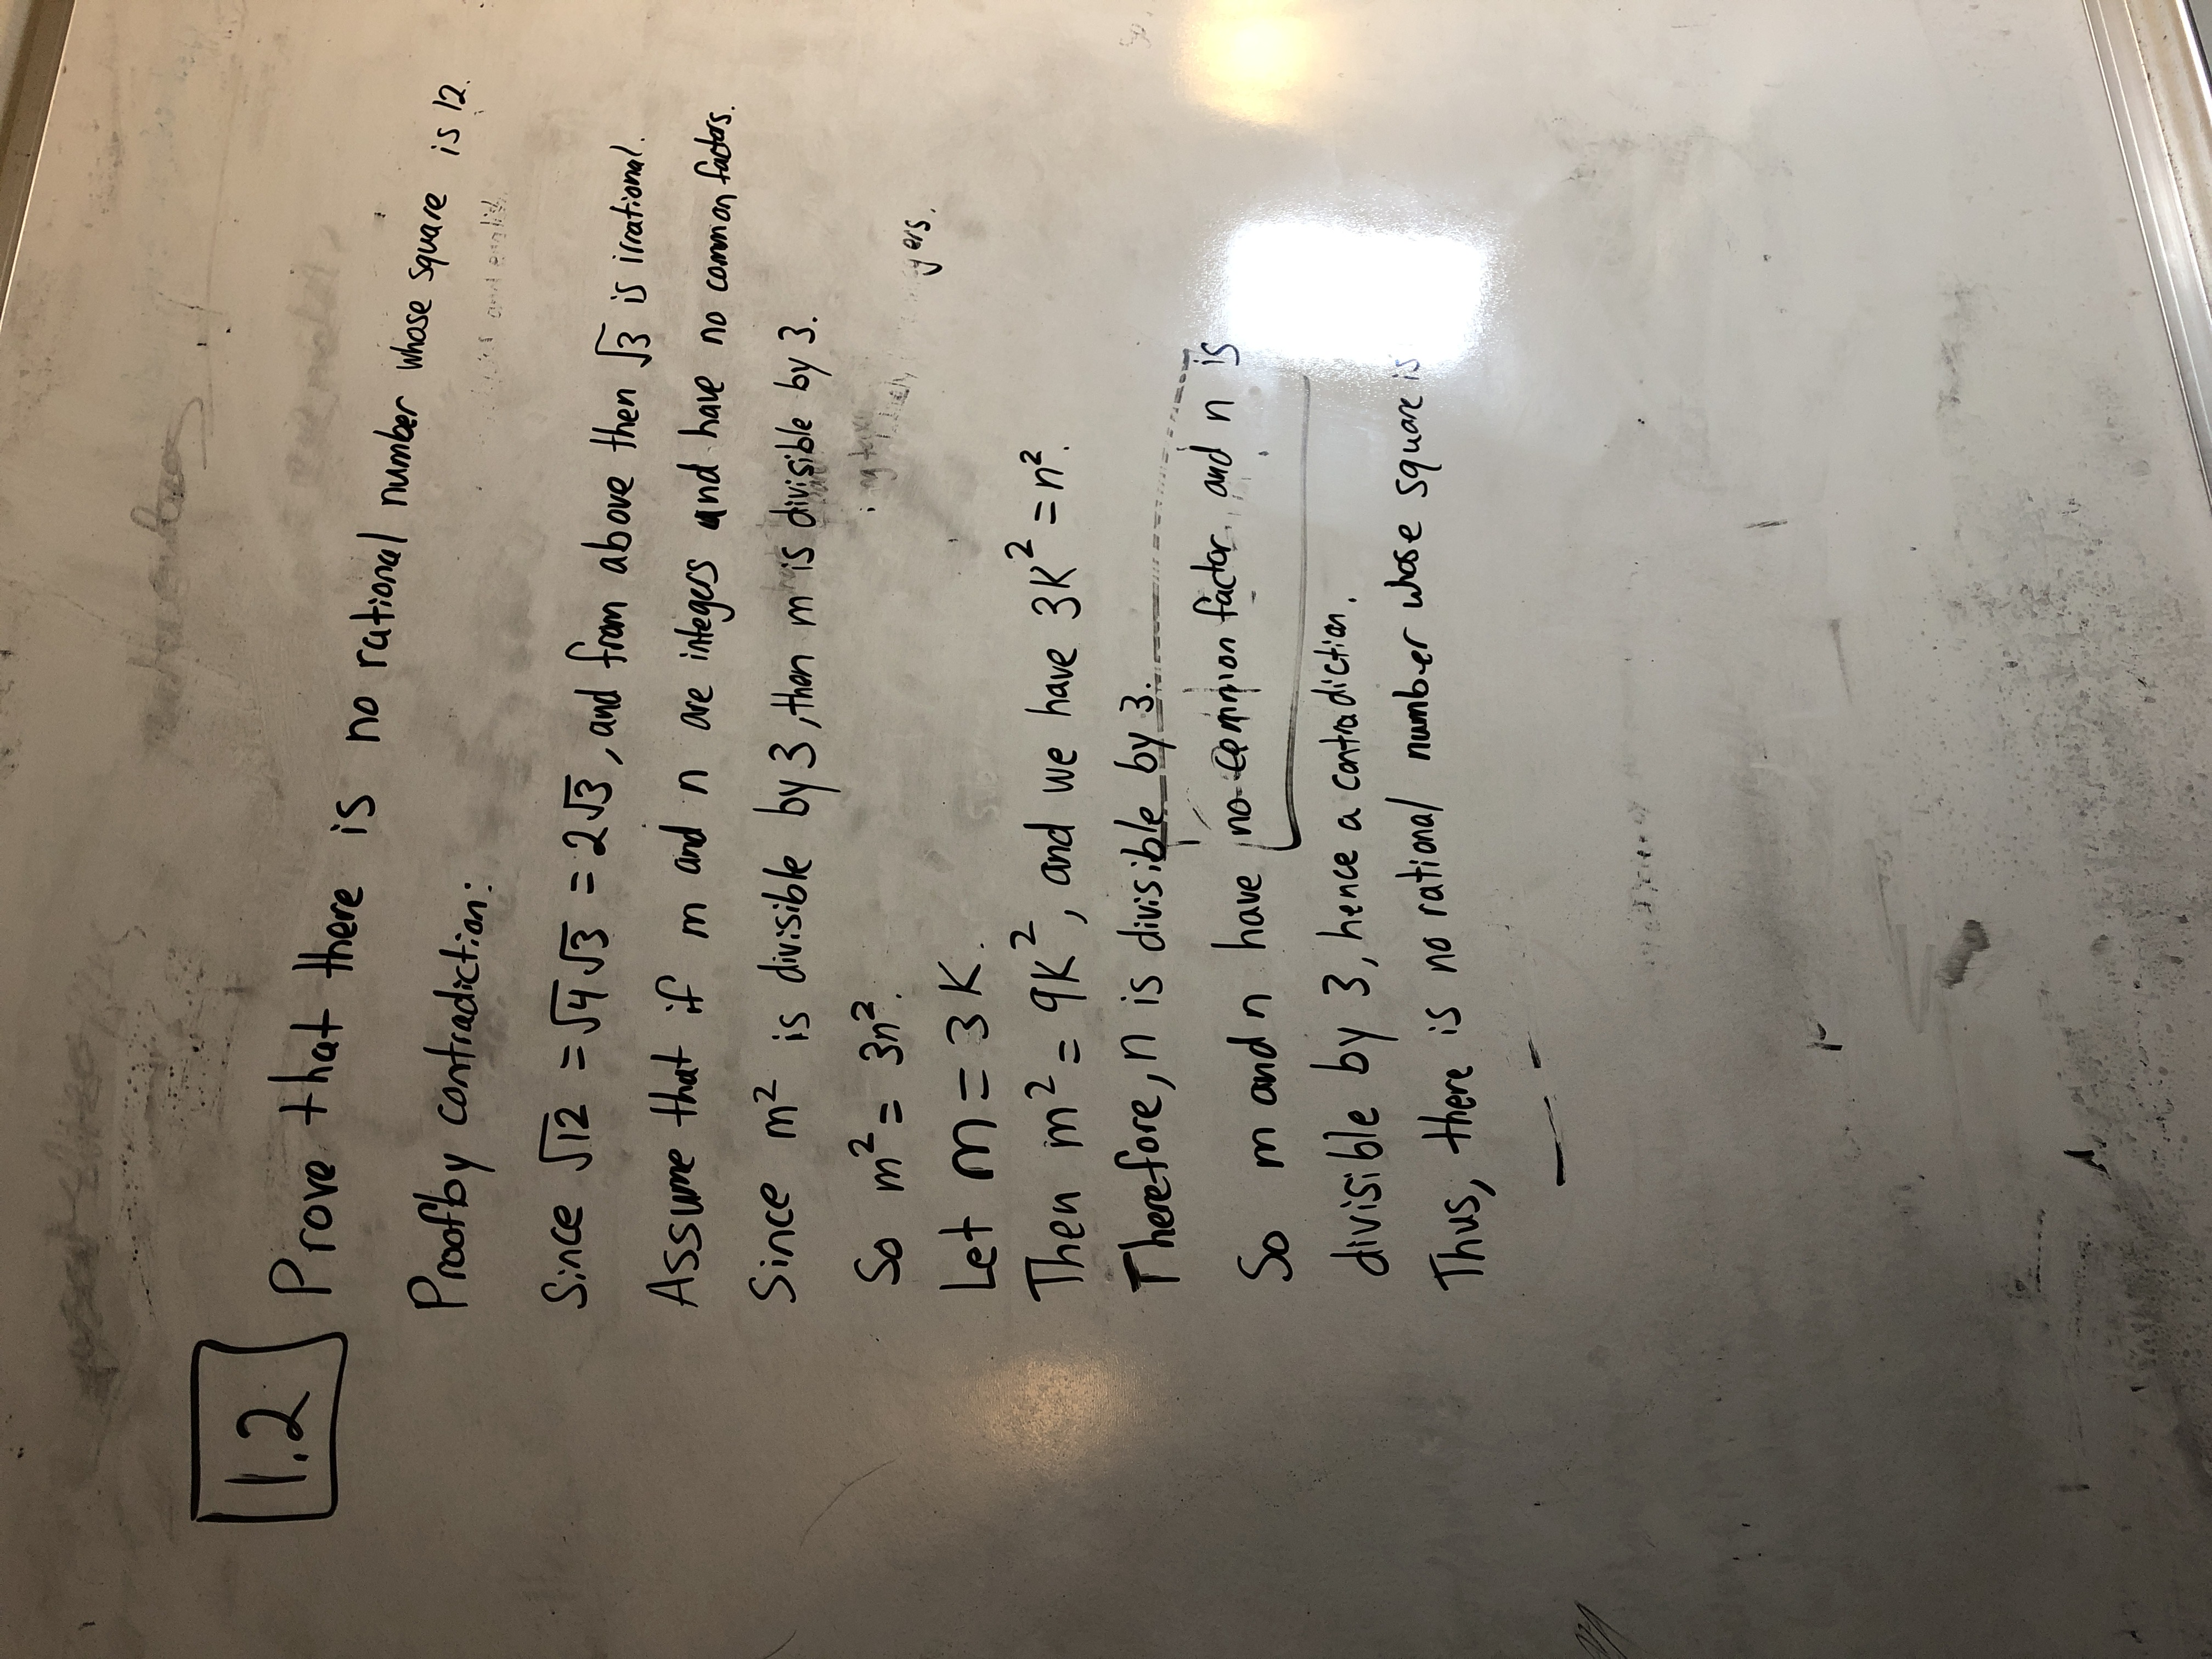
\includegraphics[angle=, origin=c,width=2.5 in]{Figures/IMG_1077.JPG}
\caption{Placeholder for bifurcation diagram proofs...preliminary angry proof} \label{fig:Euler_pic}\end{center}\end{figure} 



\newpage 
\section{Chapter 3 Baby Rudin}

\section*{Problem 3.1}
Prove that the convergence of ${s_n}$ implies convergence of $|{s_n|}.$ Is the converse true? 
\\
Proof:\\ 
If ${s_n}$ converges, there exists s $\in R$ such that for all $\epsilon>0,$ there exists N>0 such that for all $n \geq N, |s_n -s|< \epsilon.$ Given $ \epsilon>0,$ choose N as above. Using the reverse triangle inequality, for all $n \geq N, ||S_n|-|s||\leq |s_n -s|< \epsilon.$ \\ 
This means that ${|s_n|} converges to |s|.$\\ 
To prove that the converse is false, let $s_n=1$ if n is odd and $s_n=-1$ if n is even. Then ${s_n}$ does not converge, but $|s_n|=1$ for all n, so ${|s_n}|$ converges to 1.\\ 

\section*{Problem 3.2}
Calculate $lim_{n \rightarrow \infty} (\sqrt{n^2+n}-n)$\\ 
Proof: \\ 
$lim_{n \rightarrow \infty} (\sqrt{n^2+n}-n)$=$lim_{n \rightarrow \infty} (\sqrt{n^2+n}-n) \frac{(\sqrt{n^2+n}-n)}{(\sqrt{n^2+n}-n)}$\\ 
$lim_{n \rightarrow \infty} (\sqrt{n^2+n}-n)$=$lim_{n \rightarrow \infty}  \frac{(n^2+n-n^2)}{(\sqrt{n^2+n}+n)}$\\
$lim_{n \rightarrow \infty} (\sqrt{n^2+n}-n)$=$lim_{n \rightarrow \infty}  \frac{n}{n\sqrt{1+\frac{1}{n}}+n}$\\
$lim_{n \rightarrow \infty} (\sqrt{n^2+n}-n)$=$lim_{n \rightarrow \infty}  \frac{1}{n\sqrt{1+\frac{1}{n}}+1}$\\
$lim_{n \rightarrow \infty} (\sqrt{n^2+n}-n)$=$\frac{1}{2}$\\
\subsection*{Problem 3.3}
If $s_1=\sqrt{2},$ and $s_{n+1}=\sqrt{2+\sqrt{s_n}}$ where $n=(1,2,3,...),$ prove that ${s_n}$ converges, and that $s_n<2$ for $(n=1,2,3...).$\\ 
Key Definition: If a sequence is bounded and monotone then it converges.\\ 
Proof: \\ 
We know $s_q=\sqrt{2}<2.$\\ 
If $s_n<2,$ then $\sqrt{s_n}<\sqrt{2}.$ \\ 
So $s_{n+1}=\sqrt{2+\sqrt{s_n}}<\sqrt{2+\sqrt{2}}=2.$\\ 
Thus, by induction, $s_n<2$ for all n. \\ 
Need to prove $s_{n+1}>s_n$. \\ 
We know $s_q=\sqrt{2},$ so $s_2=\sqrt{2+\sqrt{2}}>\sqrt{2}=s_1.$\\ 
If we assume $s_{n-1}<s_n,$ then we have $\sqrt{s_{n-1}<\sqrt{s_n}}.$\\ 
$0>\sqrt{s_{n-1}}-\sqrt{s_n}.$\\ $2>2+\sqrt{s_{n-1}}-\sqrt{s_n}.$\\ 
$2>s_{n}^2-\sqrt{s_n}.$\\ 
$2+\sqrt{s_n}>s_{n}^2. $\\ 
$s_{n+1}=\sqrt{2+\sqrt{s_n}}>s_n.$\\ 
Thus, by induction, $s_1<s_2<....$ \\ 
This means ${s_n}$ is monotone increasing and bounded by 2. \\
Hence, by theorem 3.14, ${s_n}$ converges.
\section*{Problem 3.4}
Find the upper and lower limits of the sequence ${s_n}$ defined by $s_1=0; s_{2m}=\frac{s_{2m-1}}{2}; s_{2m+1}=\frac{1}{2}+s_{2m}.$\\ 
Proof: \\ 
By induction, $s_{2m}=\frac{1}{2}-\frac{1}{2^m}$ and $s_{2m+1}=1-\frac{1}{2^m}.$ for m=1,2,.... The second of these equalities is a direct consequence of the first, and so we need only prove the first. Immediate computation shows that $s_2=0$ and $s_3=\frac{1}{2}.$ \\ 
Hence assume that both formulas hold for $m \leq r.$\\ 
Then $s_{2r+2}=\frac{1}{2}s_{2r+1}.$\\ 
$s_{2r+2}=\frac{1}{2}(1-\frac{1}{2^r}).$\\
$s_{2r+2}=\frac{1}{2}-\frac{1}{2^{r+1}}.$\\\\ 
Thus, by induction it is proved. \\ 
Therefore, we have $lim_{n \rightarrow \infty}sup s_n=1$ and $lim_{n \rightarrow \infty}inf s_n=\frac{1}{2}.$
\subsection*{Problem 3.5}
For any two real sequences ${a_n},{b_n}$ prove that $lim_{n \rightarrow \infty} sup(a_n +b_n)\leq lim_{n \rightarrow \infty}a_n$+ $lim_{n \rightarrow \infty}sup b_n,$ provided the sum on the right is not of the form $\infty-\infty.$\\ 
Proof: \\ 
Let ${n_k}$ be a sequence in $N$ such that $lim_{k \rightarrow \infty} (a_{n_k}+b_{n_k})=lim sup(a_n +b_n).$\\ 
Let A and B be the sets of subsequential limits of $a_{n_k}$ and $b_{n_k}$ respectively. \\ 
Then $lim sup (a_n +b_n)= lim_{k \rightarrow \infty} (a_{n_k}+b_{n_k}) \leq sup A+ sup B \leq lim sup a_n + lim sup b_n.$

\newpage
\section{Unedited Problem set}

\section*{6}
Investigate the behavior (convergence or divergence) of $\sum a_n$ if \\ 
$(a) a_n= \sqrt{n+1}-\sqrt{n}$\\ 
$a_n= (\sqrt{n+1}-\sqrt{n}) (\frac{\sqrt{n+1}+\sqrt{n}}{\sqrt{n+1}+\sqrt{n}})$
\\
$a_n= \frac{n+1-n}{\sqrt{n+1}+\sqrt{n}}$
\\
$a_n=\frac{1}{\sqrt{n+1}+\sqrt{n}}$
\\ 
Since $a_n=\frac{1}{\sqrt{n+1}+\sqrt{n}}>\frac{1}{2\sqrt{n+1}},$ the series $\sum a_n$ where the p-series is p=$\frac{1}{2}$ so it diverges by the comparison test. 
(b) $a_n= \frac{\sqrt{n+1}-\sqrt{n}}{n}$
\\ 
$a_n=\frac{\sqrt{n+1}-\sqrt{n}}{n}$ 
\\
$a_n= (\frac{\sqrt{n+1}-\sqrt{n}}{n})(\frac{\sqrt{n+1} +\sqrt{n}}{\sqrt{n+1}+\sqrt{n}})$ \\

$a_n = \frac{1}{n(\sqrt{n+1}+\sqrt{n})}$
\\ 
Since $a_n = \frac{1}{n(\sqrt{n+1}+\sqrt{n})}>\frac{1}{n^\frac{3}{2}}$ the series converges by the comparison test where the p-series is $p=\frac{3}{2}.$
\\
(c)$a_n=(n^\frac{1}{n}-1)^n$
Since $(a_n)^\frac{1}{n}=n^\frac{1}{n}-1,$ then by the root test as $n \longrightarrow \infty$ the series converges. \\ 
(d)
$(d) a_n = \frac{1}{1+z^n}$ for complex values of z. \\ 
If $|z|>1,$ the series converges by comparison with a geometric series with $r= \frac{1}{|z|}<1.$ If $|z|\leq 1,$ then $|a_n| \geq \frac{1}{2},$ so that $a_n$ does not tend to zero. Hence the series diverges. 

\section*{7}
Prove that the convergence of $\sum \frac{\sqrt{a_n}}{n}$ if $a_n \geq 0.$\\ 
Since $(\sqrt{a_n}-\frac{1}{n})^2 \geq 0,$ then  
$\frac{\sqrt{a_n}}{n}\leq \frac{1}{2}(a_n^2+\frac{1}{n^2}).$\\ 
Next, $\sum a_n^2$ converges by the comparison test with $\sum a_n$ (since $\sum a_n$ converges, we have $a_n <1$ for large n, and hence $a_n^2<a_n.$
Since $\sum \frac{1}{n^2}$ converges (p series, p =2). 
Then by Theorem 3.47 $\sum \frac{1}{2}(a_n+\frac{1}{n^2})=\frac{1}{2}(\sum a_n +\sum \frac{1}{n^2})$ the series $\sum \frac{1}{2}(a_n+\frac{1}{n^2}$ also converges.
\\Thus, $\sum \frac{\sqrt{a_n}}{n}$ converges by the comparison test. \\ 

\section*{8}
If $\sum a_n$ converges, and if ${b_n}$ is monotonic and bounded, prove that $\sum a_n b_n$ converges. \\ 
Let $S_n =\sum_{k=1}^n a_k (S_0 =0).$ 
\\ 
Then $a_k = S_k- S_{k-1}$ for $k=1,2,....$ 
\\
Let M be an upper bound for $|b_n|$ and $|S_n|$. \\ 
Let S=$\sum a_n$ and b= lim $b_n.$ 
\\Choose N to be large in a way that the next three inequalities hold for all $m> N$ and $n> N$:\\ 
$|b_n S_n -bS|<\frac{\epsilon}{3}; |b_mS_m-bS|<\frac{\epsilon}{3}; |b_m-b_n|<\frac{\epsilon}{3M}.$\\ 
Then if $n>m>N,$ the formula for summation by parts yields, $\sum_{k=m+1}^n a_n b_n= b_nS_n-b_mS_m+\sum_{k=m}^{n-1}(b_k-b_{k+1})S_k.$\\ 
Thus, $b_nS_n-b_mS_m|<\frac{2 \epsilon}{3},$ and 
$|\sum_{k=m}^{n-1}(b_k-b_{k+1})S_k|\leq M \sum_{k=m}^{n-1}|b_k-b_{k+1}|.$ \\ 
Since the sequence ${b_n}$ is monotonic,  $\sum_{k=m}^{n-1}|b_k-b_{k+1}|=|\sum_{k=m}^{n-1}(b_k-b_{k+1})|=|b_m-b_n|<\frac{\epsilon}{3M,}$ 
from which the desired inequality follows. 
Therefore, given $\epsilon >0$ there exists N such that $| \sum_{k=m+1}^n a_kb_k|<\epsilon$ if $n> m \geq N.$ 
\\
Thus, the partial sums of the series form a Cauchy sequence.
\section*{9}
Find the radius of convergence of each of the following power series\\ 
(a)$\sum n^3 z^n,$ \\ 
The radius of convergence is 1, as $a_n=n^3$ fulfills the requirement $lim_{n \longrightarrow \infty} \frac{a_n}{a_{n+1}}=1.$\\ 
(b) $\sum \frac{2^n}{n!}z^n,$ \\
The radius of convergence is infinite, as $a_n =\frac{2^n}{n!}$ fulfills the requirement $lim_{n \longrightarrow \infty} \frac{a_n}{a_{n+1}}=lim_{n \longrightarrow \infty} \frac{n+1}{2}=\infty.$\\
(c)$\sum \frac{2^n}{n^2}z^n,$ \\
The radius of convergence is $\frac{1}{2},$ as $a_n=\frac{2^n}{n^2}$ fulfills the requirement \\ 
$lim_{n \longrightarrow \infty} \frac{a_n}{a_{n+1}}=lim_{n \longrightarrow \infty} \frac{1}{2}(1+\frac{1}{n})^2=\frac{1}{2}.$\\
(d)$\sum \frac{n^3}{3^n}z^n.$ \\ 
The radius of convergence is 3, as $a_n = \frac{n^3}{3^n}$ fulfills the requirement that \\ 
$lim_{n \longrightarrow \infty} \frac{a_n}{a_{n+1}}= lim_{n \longrightarrow \infty} 3(\frac{n}{n+1})^3=3.$\\ 
\section*{10}
Suppose that the coefficients of the power series $\sum a_n z^n$ are integers, infinitely many of which are distinct from zero. Prove that the radius of convergence is at most 1. \\ 


Due to the fact that the sequence ${a_n}$ contains infinitely many nonzero numbers. \\ 
Let ${n_k}$ be a subsequence of positive integers where $a_{n_k} \neq 0$ for all k. \\ 
Furthermore, as $a_n$ is an integer for each n, then $|a_n_k| \geq$ for each k, and thus $(|a_{n_k}|)^{n_k} \geq 1.$\\ 
Therefore, lim sup $n \longrightarrow \infty (|a_n|)^{n}\geq 1$. \\ 
Thus, R= $\frac{1}{lim sup n \longrightarrow \infty (|a_n|)^{n}} \leq 1.$ So the radius of convergence is at most 1. 
\subsection*{Unedited Problem set}
11, 12, 16,17 ,18
\section*{11}
Suppose $a_n > 0, s_n =a_1 + \dots +a_n,$ and $\sum a_n$ diverges. \\ 
(a) Prove that $\sum \frac{a_n}{1+a_n}$ diverges. \\ 
If $a_n$ does not remain bounded, then $\frac{a_n}{1+a_n}$ does not tend to zero, and hence the series $\sum \frac{a_n}{1+a_n}$ diverges. If $a_n \geq M$ for all n, then $\frac{a_n}{1+a_n}\leq \frac{1}{1+M}a_n,$ and hence again the series is divergent. \\ 
(b) Prove that $\frac{a_{n+1}}{s_{n+1}}+ \dots \frac{a_{n+k}}{s_{n+k}} \leq 1- \frac{S_N}{s_{n+k}}$ and deduce that $\sum \frac{a_n}{S_n}$ diverges. \\
Replacing each denominator on the left by $s_{N+k}$,we have $\frac{a_{N+1}}{S_{N+1}}+ \dots \frac{a_{N+k}}{s_{N+k}}$ $\geq \frac{1}{S_{N+k}}(A_{N+1}+a_{N+2}+ \dots +a_{N+k}=$  $\frac{1}{s_{N+k}}(S_{N+k}-s_N)$=$1-\frac{S_N}{S_{N+k}}$.\\ 
It follows that the partial sums of the series $\sum \frac{a_n}{s_n}$ do not form a Cauchy sequence. For, no matter how large N is taken, if N is held fixed, the right hand side can be made larger than $\frac{1}{2}$ by taking k sufficiently large (since $S_{N+k} \longrightarrow \infty ).$
(c)Prove that $\frac{a_n}{s_n^2}\leq \frac{1}{s_{n-1}}-\frac{1}{s_n}$ and deduce that $\sum \frac{a_n}{s_n^2}$ converges. \\ 
We observe that if $n \geq 2,$ then \\ 
$\frac{1}{s_{n-1}}-\frac{1}{s_n}=\frac{s_n -s_{n-1}}{s_{n-1}s_n}= \frac{a_n}{s_{n-1}s_n}\geq \frac{a_n}{s_n^2}.$\\ 
Since the series $\sum_{n=2}^\infty \frac{1}{s_{n-1}}-\frac{1}{s_n}$ converges to $\frac{1}{a_1,}$ it follows by comparison that $\sum \frac{a_n}{s_n^2}$ converges. Or in other words it is a telescoping series.\\ 
(d)What can be said about $\sum \frac{a_n}{1+na_n}$ and $\sum \frac{a_n}{1_n^2 a_n}$?\\ 
The series $\sum \frac{a_n}{1+na_n}$ may either be convergent or divergent. If the sequence ${na_n}$ is bounded above or has a positive lower bound, it definitely diverges. Thus if $na_n \leq M,$ each term is at least $\frac{1}{1+M}a_n,$ and so the series diverges. If $na_n \geq \epsilon >0$ for all n, then each term is at least $\frac{\epsilon}{1+\epsilon}\frac{1}{n},$ and once again the series is divergent. \\ 
In general, however, the series $\sum \frac{a_n}{1+na_n}$ may converge. For example let $a_n= \frac{1}{n^2}$ if n is not a perfect square and $a_n= \frac{1}{\sqrt{n}}$ if n is a perfect square. The sum of $\frac{a_n}{1+na_n}$ over the nonsquares obviously converges by comparison with the p series, p=2. As for the sum over the square integers it is $\sum \frac{1}{n+n^2}$ which converges by comparison with p series, p=2. \\ 
Finally, the series $\sum \frac{a_n}{1+n^2 a_n}$ is obviously majorized by the p series with p=2, hence converges. \\ 
\section*{12}
Suppose $a_n>0$ and $\sum a_n$ converges. Put $r_n= \sum_{m=n}^\infty a_n.$ \\ 
(a) Prove that $\frac{a_m}{r_m}+ \dots +\frac{a_n}{r_n}>1-\frac{r_n}{r_m}$ if $m<n$, and deduce that $\sum \frac{a_n}{r_n}$ diverges. \\ 
(a) Replacing all the denominators on the left-hand side by the largest one $(r_m)$, we find \\ 
$\frac{a_m}{r_m}+ \dots + \frac{a_n}{r_n}> \frac{a_m + \dots +a_n}{r_m}= \frac{r_m-r_{n+1}}{r_m}>1-\frac{r_n}{r_m},$ since $r_n > r_{n+1}.$\\ 
Just like in problem 11, this keeps the partial sums of the series $\sum \frac{a_n}{r_n}$ from forming a Cauchy sequence. No matter how large m is taken, one can choose n larger so that the difference $\sum_{k=m}^n \frac{a_k}{r_k}$ is at least $\frac{1}{2}$, since $r_n \longrightarrow 0$ as $n \longrightarrow \infty.$ \\ 
(b)Prove that $\frac{a_n}{\sqrt{r_n}}<2(\sqrt{r_n -\sqrt{r_{n+1})}}$ and deduce that $ \sum \frac{a_n}{\sqrt{r_n}}$ converges. 


We have $\frac{a_n}{\sqrt{r_n}}(\sqrt{r_n}+\sqrt{r_{n+1}})= a_n +a_n \frac{\sqrt{r_{n+1}}}{\sqrt{r_n}}<2a_n=2(r_n -r_{n+1}).$ Dividing both sides by $\sqrt{r_n}+\sqrt{r_{n+1}}$ now yields the desired inequality. Since the series $\sum (\sqrt{r_n}-\sqrt{r_{n+1}})$ converges to $\sqrt{r_1},$ it follows by comparison that $\sum \frac{a_n}{\sqrt{r_n}} converges. $ \\

\section*{16}\\ 
Fix a positive number $\alpha.$ Choose $x_1> \sqrt{\sqrt{\alpha}},$ and define $x_1, x_2, x_3,...,$ by the recursion formula $x_{n+1}=\frac{1}{2}(x_n +\frac{\alpha}{x_n}).$\\ 
(a) Prove that ${x_n}$ decreases monotonically and that $lim x_n = \sqrt{\alpha}.$\\ 
We note that $x_n$ is always positive, and that if $x_n > \sqrt{\alpha},$ then $x_{n+1}^2-\alpha =\frac{1}{4}(x_n - \frac{\alpha}{x_n})^2 >0.$ Thus, $x_n > \sqrt{\alpha}$ for all n. Since $x_n > \sqrt{\alpha},$ it follows that $\frac{\alpha}{x_n}<\sqrt{\alpha}<x_n.$ Hence $x_n - x_{n+1}=\frac{1}{2}(x_n-\frac{\alpha}{x_n})>0,$ and so ${x_n}$ decreases to a limit $\lambda \geq \sqrt{\alpha}.$\\ 
(b) Put $\epsilon =x_n- \sqrt{\alpha},$ and show that $\epsilon_{n+1}= \frac{\epsilon _n ^2}{2 x_n}<\frac{\epsilon_n^2}{2 \sqrt{\alpha}}$ so that, setting $\beta=2 \sqrt{\alpha},$
$\epsilon_{n+1}< \beta(\frac{\epsilon_1}{\beta})^{2^n} (n=1,2,3,...,).$\\ 
We have $\frac{\epsilon_n^2}{2x_n}=\frac{x_n^2-2x_n \sqrt{\alpha}+\alpha}{2x_n}=\frac{1}{2}(x_n + \frac{\alpha}{x_n})- \sqrt{\alpha}=x_{n+1}-\sqrt{\alpha}=\epsilon_{n+1}.$\\ 
The inequality then results from the simple fact that $x_n > \sqrt{\alpha.}$ Thus $\epsilon_2< \frac{\epsilon_1 ^2}{\beta}= \beta (\frac{\epsilon_1}{\beta})^2.$ \\ 
By induction, if we suppose that $\epsilon_n < \beta (\frac{\epsilon_1}{\beta})^{2^{n-1}},$ we find $\epsilon_{n+1}<\frac{\epsilon_n^2}{\beta}<\beta (\frac{\epsilon_1}{\beta})^{2^n}.$\\



(c) Since $\beta=2\sqrt{3} and \epsilon=2-\sqrt{3}, then \frac{\epsilon_1}{\beta}=\frac{2-\sqrt{3}}{2\sqrt{3}}=\frac{1}{\sqrt{3}}-\frac{1}{2}.$\\ 
Since $\frac{1}{\sqrt{3}}+\frac{1}{2}>\frac{1}{2}+\frac{1}{2},$ then $\frac{1}{\sqrt{3}}+\frac{1}{2}>1.$ \\ 
So $\frac{\epsilon_1}{\beta}(\frac{1}{\sqrt{3}}+\frac{1}{2})=(\frac{1}{\sqrt{3}}-\frac{1}{2})(\frac{1}{\sqrt{3}+\frac{1}{2}}).$\\ 
Hence, $\frac{\epsilon_1}{\beta}(\frac{1}{\sqrt{3}}+\frac{1}{2})=\frac{1}{12}.$ \\ 
Since $\frac{\epsilon_1}{\beta}(\frac{1}{\sqrt{3}}+\frac{1}{2})<\frac{1}{10} then \frac{\epsilon_1}{\beta}<\frac{1}{10}.$\\ 
Therefore from (b), $\epsilon_5< \beta (\frac{\epsilon_1}{\beta})^{2^4}<2\sqrt{3}*10^{-16}<4*10^-16.$ \\ 
With the same logic, $\epsilon_6<4*10^{-32}.$



\section*{17}\\
Fix $\alpha>1.$ Take $x_1>\sqrt{\alpha},$ and define \\ 
$x_{n+1}= \frac{\alpha +x_n}{1+x_n}=x_n +\frac{\alpha-x_n^2}{1+x_n}.$\\ 
(a) Prove that $x_1> x_3>x_5>... $\\ 
Most of the work in this problem is done by the following three identities, whose proofs are routine computations: \\ 
$(1+x_n)(1+x_{n+1})=2(1+x_n)+(\alpha -1),$ \\ 
$x_{n+1}^2 -\alpha= - [\frac{(\alpha -1)}{(1+x_n)^2}](x_n^2- \alpha),$ \\ 
$x_{n+1}^2 -\alpha= \frac{(\alpha -1)^2}{(1+x_n)^2 (1+x_{n-1})^2}(x_{n-1}^2 -\alpha)=$ \\ 
$X_{n+1}^2- \alpha=[\frac{\alpha -1}{(\alpha-1)+2(1+x_{n-1}}]^2 (x_{n-1}^2 -\alpha).$ 
The second of these identities shows that $x_n$ and $x_{n+1}$ lie on opposite sides of $\sqrt{\alpha}$. The third shows that $x_{n+1}$ is closer to $\alpha$ than $x_{n-1}.$ Hence, since $x_1> \sqrt{\alpha}$ by hypothesis, parts (a) and (b) are proved. \\ 
as for (c), the third relation shows that $|x_{n+1}^2- \alpha| \leq r^{2k}|x_n^2 -\alpha|,$ where $r= \frac{\alpha -1}{2+ \alpha -1}<1.$ It follows that $|x_{n+2k}^2-\alpha|\leq r^{2k}|x_n^2-\alpha|,$ and the right-hand side of this expression tends to zero as $k \longrightarrow \infty.$ Thus, $lim_{k \longrightarrow \infty}x_{n+2k}= \alpha $ whether n is odd or even, and so $lim_{n \longrightarrow \infty} x_n = \sqrt{\alpha}.$\\ 
The convergence in this case is geometric, but not quadratically geometric as in exercise 16. The rate of convergence will depend on the size of $\alpha.$ For $1<\alpha \leq 2$ we certainly have $ x_n \geq \alpha -2$ for all n, and so in this case $r> \frac{1}{3},$ i.e. $|x_{n+1}^2 - \alpha|< \frac{1}{9}|x_{n-1}^2- \alpha |.$ \\ 
This implies that $|x_{n+1}- \sqrt{\alpha}|< \frac{1}{9} \frac{x_{n-1}+ \sqrt{\alpha}}{x_{n+1}+\sqrt{\alpha}}|.$ \\ 
If n is even, we can at least assume $x_1 <1.5$ (since $\alpha \leq 2),$ and so  $\frac{x_{n-1}+\sqrt{\alpha}}{x_{n+1}+\sqrt{\alpha}}<1.5,$so that $|x_{n+1}-\sqrt{\alpha}|<\frac{1.5}{9}|x_{n-1}-\alpha|.$ \\ 

\section*{18}
Replace the recursion formula from problem 16 by $x_{n+1}=\frac{p-1}{p}x_n + \frac{\alpha}{p}x_n^{-p+1},$ where p is a fixed positive integer, and describe the behavior of the resulting sequences ${x_n}.$ \\ 
(Exercise 16 is the case p=2 of course.) \\ 
The main work is done by the following easily derived formulas, which hold if $x_n > \alpha ^\frac{1}{p}.$ \\ 
$x_{n+1}- \alpha ^\frac{1}{p}= (x_n - \alpha^ \frac{1}{p})[(\frac{p-1}{p})-\frac{1}{p}((\frac{\alpha^\frac{1}{p}}{x_n})+ \dots + (\frac{\alpha^\frac{1}{p}}{x_n})^{p-1}))]$\\ 
$x_{n+1}- \alpha ^\frac{1}{p}< (x_n- \alpha ^\frac{1}{p})(\frac{p-1}{p})(1-(\frac{\alpha^\frac{1}{p}}{x_n}^{p-1}) $ \\ 
$x_{n+1}- \alpha ^\frac{1}{p}= (x_n- \alpha ^\frac{1}{p})(\frac{p-1}{px_n^{p-1}})(x_n^{p-1}-(\alpha ^\frac{1}{p})^{p-1})$ \\ 
$x_{n+1}- \alpha ^\frac{1}{p}= (x_n- \alpha ^\frac{1}{p})^2 (\frac{p-1}{px_n^{p-1}})[x_n^{p-2}+x_n^{p-3}\alpha ^\frac{1}{p}+ ...+ \alpha^ \frac{p-2}{p}]$ \\ 
$x_{n+1}- \alpha ^\frac{1}{p}< (x_n- \alpha ^\frac{1}{p})^2 (\frac{(p-1)^2}{p x_n})$ \\ 
$x_{n+1}- \alpha ^\frac{1}{p}< (x_n- \alpha ^\frac{1}{p})^2 (\frac{(p-1)^2}{p \alpha ^\frac{1}{p}})$. \\ 
Thus, we can guarantee quadratic-geometric convergence if we start with $x_1 - \alpha ^\frac{1}{p}= \epsilon_1 < \beta = \frac{p \alpha ^ \frac{1}{p}}{(p-1)^2}.$ In that case we obtain the same inequalities as in exercise 16, and $x_n \longrightarrow \alpha ^\frac{1}{p}.$

\section{The Third Compilation}
\section*{Me Pontificating}

\section*{1}
(10 points) Prove, without using derivatives and without using the Fundamental Theorem of Algebra, that the polynomial $x^3-777x^2+5672x+952320$ has at least three roots. 
\\
Let $f(x)=x^3-777x^2+5672x+952320.$ \\ 
There are 2 sign changes in f(x). \\ 
Therefore f has two positive real roots. \\ 
Then $f(-x)=-x^3-777x^2-5672x+952320.$\\ 
Then there is 1 sign change in $f(-x).$ \\ 
Thus, f has one negative real root. \\ 
Hence, f has three real roots. 
\subsection*{1.1 Me pontificating}


\begin{figure}[h]\begin{center}\includegraphics[angle=, origin=c,width=2 in]{WhiteboardPictures/Exam 2/IMG_1052.JPG}
\caption{Placeholder for my proofs} \label{fig:Euler_pic}\end{center}\end{figure} 

\newpage


\subsection*{2}
(10 points) Suppose that the function f(x) is defined on $R^1,$ that f(x) is continuous at $x=-9,$ that f(5)=-100, and that for all real x and y, $f(x+y)=f(x)+f(y).$ \\ 
Find an explicit, closed-form expression for f(x). \\ 
Establish that there is one, and only one, such function; that is, prove that the function is unique. \\ 
Compute $f(-3).$ \\ 
Prove your conclusions. \\ 



$f(x+y)=f(x)+f(y).$ \\ 
Let $y=-x$ then \\ 
$f(0)=f(x)+f(-x).$ \\ 
Let $y=x,$ then \\ 
$f(2x)=2f(x)$ \\ 
$f(0)=2f(0)$ \\ $f(0)=0.$ \\
So $f(0)=f(x)+f(-x)$ \\ 
$0=f(x)+f(-x)$ \\ 
$f(x)=-f(-x)$\\ 
Now, $f(x+y)=f(x)+f(y)$ \\ 
Let $x= \gamma-5$ and $y=5,$ then \\ 
$f(\gamma)=f(\gamma-5)+f(5)$ and $f(\gamma-5)=f(\gamma-10)+f(5).$ \\ 
So $f(\gamma)= f(\gamma -10)+f(5)+f(5)$ \\ 
$= f(\gamma-5*2)+2f(5)$ \\ 
We can generalize as $f(\gamma)=f(\gamma-5\gamma)+\gammaf(5).$ \\ 
$f(\gamma)= f(-4 \gamma) + \gamma f(5).$ \\
Now $f(2x)=2f(x).$ \\ 
Let $x=-2\gamma$ then \\ 
$f(-4 \gamma)=2 f(-2 \gamma)$ --> 1. 
If we put n=-r then. \\ 
$f(-2r)=2f(-r).$ -->2 \\ 
From 1 and 2 we get 
$f(-4 \gamma)=2[2f(-\gamma)]]$ \\ 
=$\Deltaf(-\gamma)$. \\ 
And $f(x)=-f(-x)$. \\ 
So $f(- \gamma))=-f(\gamma).$ \\ 
So $f(-4\gamma)=-4f(\gamma)$ \\ 
So $f(\gamma=f(-4 \gamma)+ \gammaf(5)$ \\
$= - \Delta f(\gamma) +\gamma(5)$ \\ 
$f(\gamma)=\frac{\gamma}{5}f(5)=-20 \gamma$ \\ 
So $f(x)=-20x$ and $f(-3)=60.$

\newpage 
\subsection*{Me pontificating}

\begin{figure}[h]\begin{center}\includegraphics[angle=, origin=c,width=2 in]{WhiteboardPictures/Exam 2/IMG_1052.JPG}
\caption{Placeholder for my proofs} \label{fig:Euler_pic}\end{center}\end{figure} 

\newpage




\section*{3}
(10 points) Towns A and B are about 20 miles distant from each other out on the perfectly flat Great Plains. There are two roads that connect the towns, Road 1 and Road 2. On Monday, Alice and Bob set out from town A to town B, Alice on Road 1 and Bob on Road 2.  They are tethered to one another by a 20-foot-long rope, because they are in a math problem.   Alice and Bob make it all the way from Town A to Town B, tethered.  The next day, Tuesday, two identical trucks, Truck $\alpha$ and Truck $\beta$, leave from different towns—Truck $\alpha$ from Town A, and Truck $\beta$ from Town B--on different roads--Truck $\alpha$ on Road 1, and Truck $\beta$ on Road 2—each headed toward the other town, at exactly the same time.  Each truck has, strapped firmly to its flatbed, again because they’re in a math problem, a perfectly spherical globe of radius 11 feet.  Is it possible for Truck $\alpha$ to make it to Town B and for Truck $\beta$ to make it to Town A? Argue clearly for your conclusion. 
\\ 

It is give that Alice and Bob set out to move from Town A to Town B, Alice on Road 1 and Bob on Road 2. They are tethered to one another by a 20-foot-long rope(as they are in a math problem). \\
Alice and Bob make all the way from Town A to Town B, tethered. \\ 
This means there was a perfect gap of 20-foot between Road 1 and Road 2. \\
However, Truck $\alpha$ and Truck $\beta$ have strapped firmly to its flatbed, a perfectly spherical globe of radius 11 feet. This means they occupy diameter $11 x 2=22$ feet each. \\ 
So even though Truck $\alpha$ starts from town A on Road 1 heading towards town B and Truck $\beta \beta$ heads from town B on Road 2 towards town A, it is not guaranteed to reach their destinations since these two truck require minimum $22+22=44$ feet at least. But from the experience of Alice and Bob they have at most 20 feet. \\ 
Thus it is not possible for the trucks to reach their destination. 

\subsection*{Me pontificating}


\begin{figure}[h]\begin{center}\includegraphics[angle=, origin=c,width=2 in]{WhiteboardPictures/Exam 2/IMG_1052.JPG}
\caption{Placeholder for my proofs} \label{fig:Euler_pic}\end{center}\end{figure} 

\section*{4}
(10 points) Prove, without using the Fundamental Theorem of Algebra, (you're welcome to use derivatives for this one, if you'd like to), that an nth degree real polynomial has at most n real roots. 
\\ 
Proposition- Any n degree polynomial having more than n distinct roots is identically 0. \\ 

Proof: \\ 
Let n=0, i.e. let b(x)= constant. \\ 
So proposition is trivially true for this case n=0. \\ 
Let the prop. holds for all poly. of degree at most $(n-1).$ \\ 
Let $b(x)=be$ a poly. of degree n. And let it has roots, $x_1, x_2, ..., x_n, x_{n+1}$ (all distinct) then by factor thm. \\ 
$b(x)=(x-x_{n+1})$q(x), q(x) is of degree $(n-1).$ \\ 
Now for $x_i, i=1,2,...,n,$ \\ 
$b(x_i)=(x_i -x_{n+1})q(x(i)$ \\ 
$0=(x_i-x_{n+1})q(x_i)$ \\ 
$q(x_i)=0$ \\ 
Therefore $x_i-x_{n+1} \neq 0.$ \\ 
q has (at least) n distinct roots. 
But it was of degree $(n-1)$\\ 
So q(x) =0 for all x. \\ 
So b(x)=0 for all x. \\ 
Hence the proposition holds for n degree polynomials too. \\ 
So the proposition holds for all polynomials. \\ 

\subsection*{Me Pontificating}
\begin{figure}[h]\begin{center}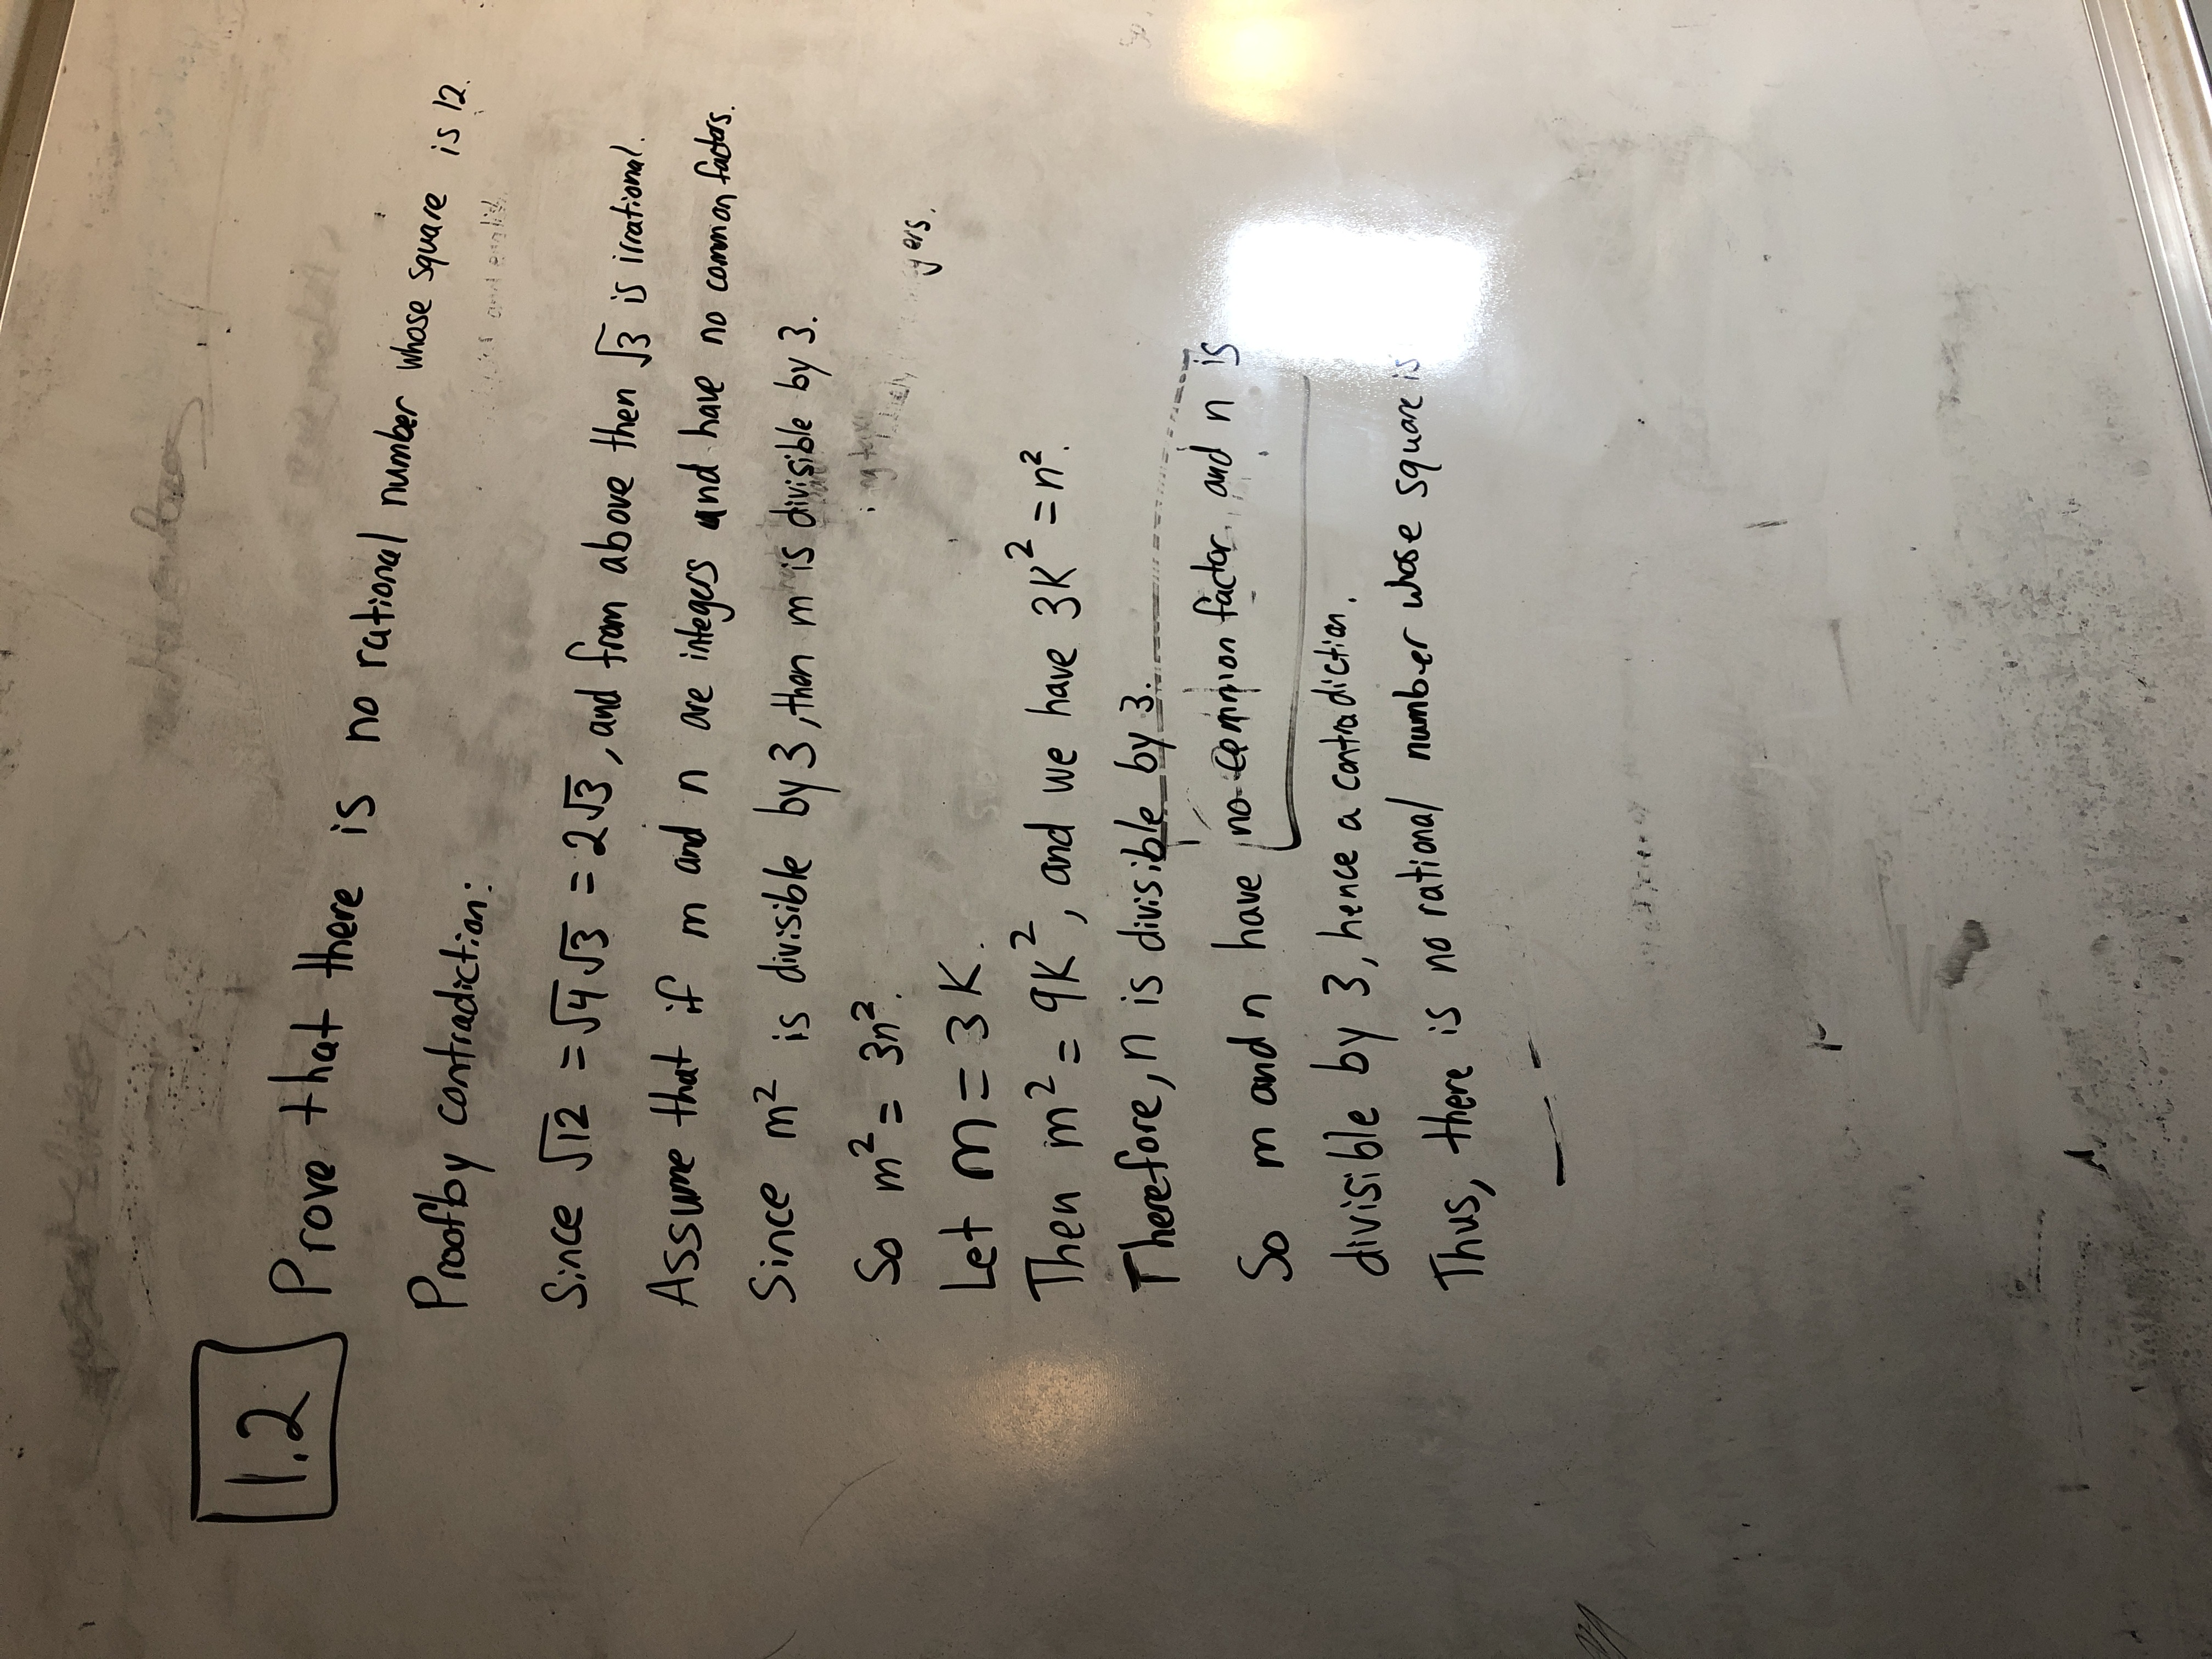
\includegraphics[angle=, origin=c,width=2 in]{Figures/IMG_1077.JPG}
\caption{Placeholder for my proofs} \label{fig:Euler_pic}\end{center}\end{figure} 

\newpage
\section*{5}
(10 points total) Consider the function on $[0,1]$ defined by $f(x)= {x}$ if x is rational 1-x if x is irrational. \\ 
Determine all points at which f(x) is continuous and all points at which it is not continuous.

\begin{figure}[h]\begin{center}\includegraphics[angle=, origin=c,width=2 in]{WhiteboardPictures/Exam 2/IMG_1052.JPG}
\caption{Placeholder for my proofs} \label{fig:Euler_pic}\end{center}\end{figure} 
\newpage

Determine whether f(x) is invertible. Prove all of your conclusions. 

\begin{figure}[h]\begin{center}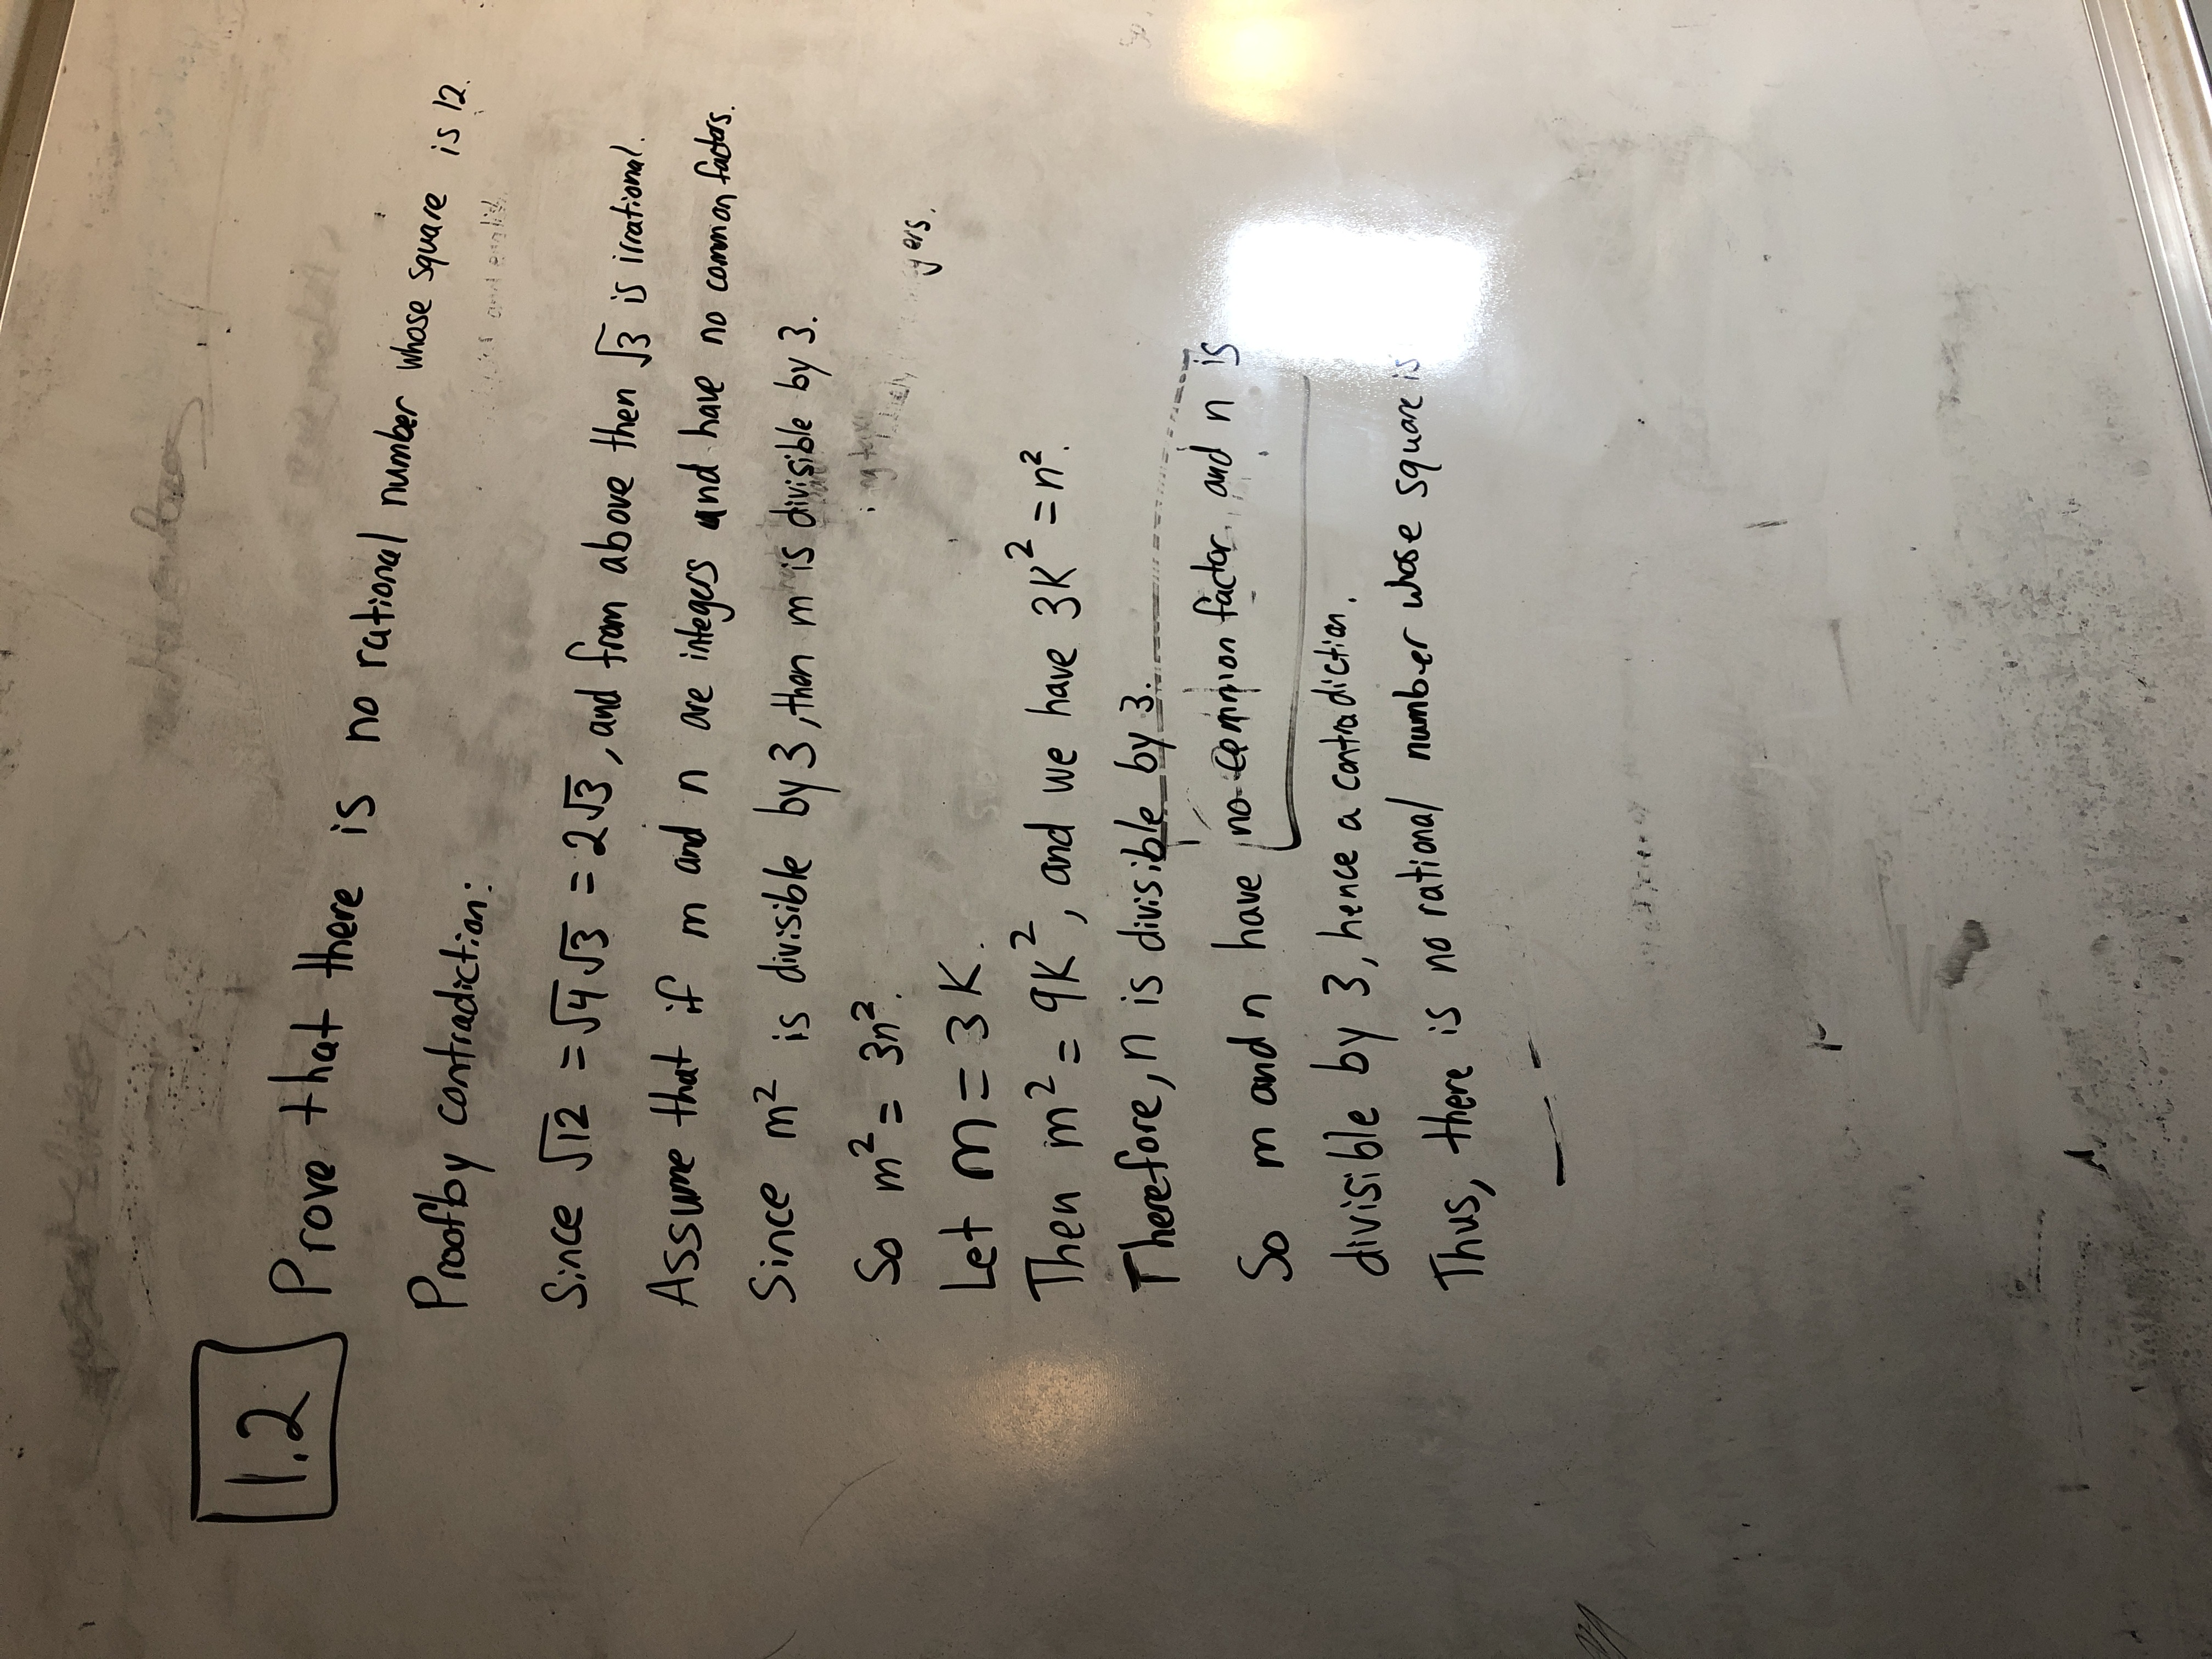
\includegraphics[angle=, origin=c,width=2 in]{Figures/IMG_1077.JPG}
\caption{Placeholder for my proofs} \label{fig:Euler_pic}\end{center}\end{figure} 


\section*{6}
(25 points) 
Let f(x) be continuous on the interval $[a,b].$ Define g(x) so that g(a)= f(a) and, for $x \in (a,b], g(x)$ is the maximum of f(s) for $a \leq s \leq x.$ \\ 
\newpage
Show that g(x) is continuous on the interval $[a,b].$ (5 points) 
\begin{figure}[h]\begin{center}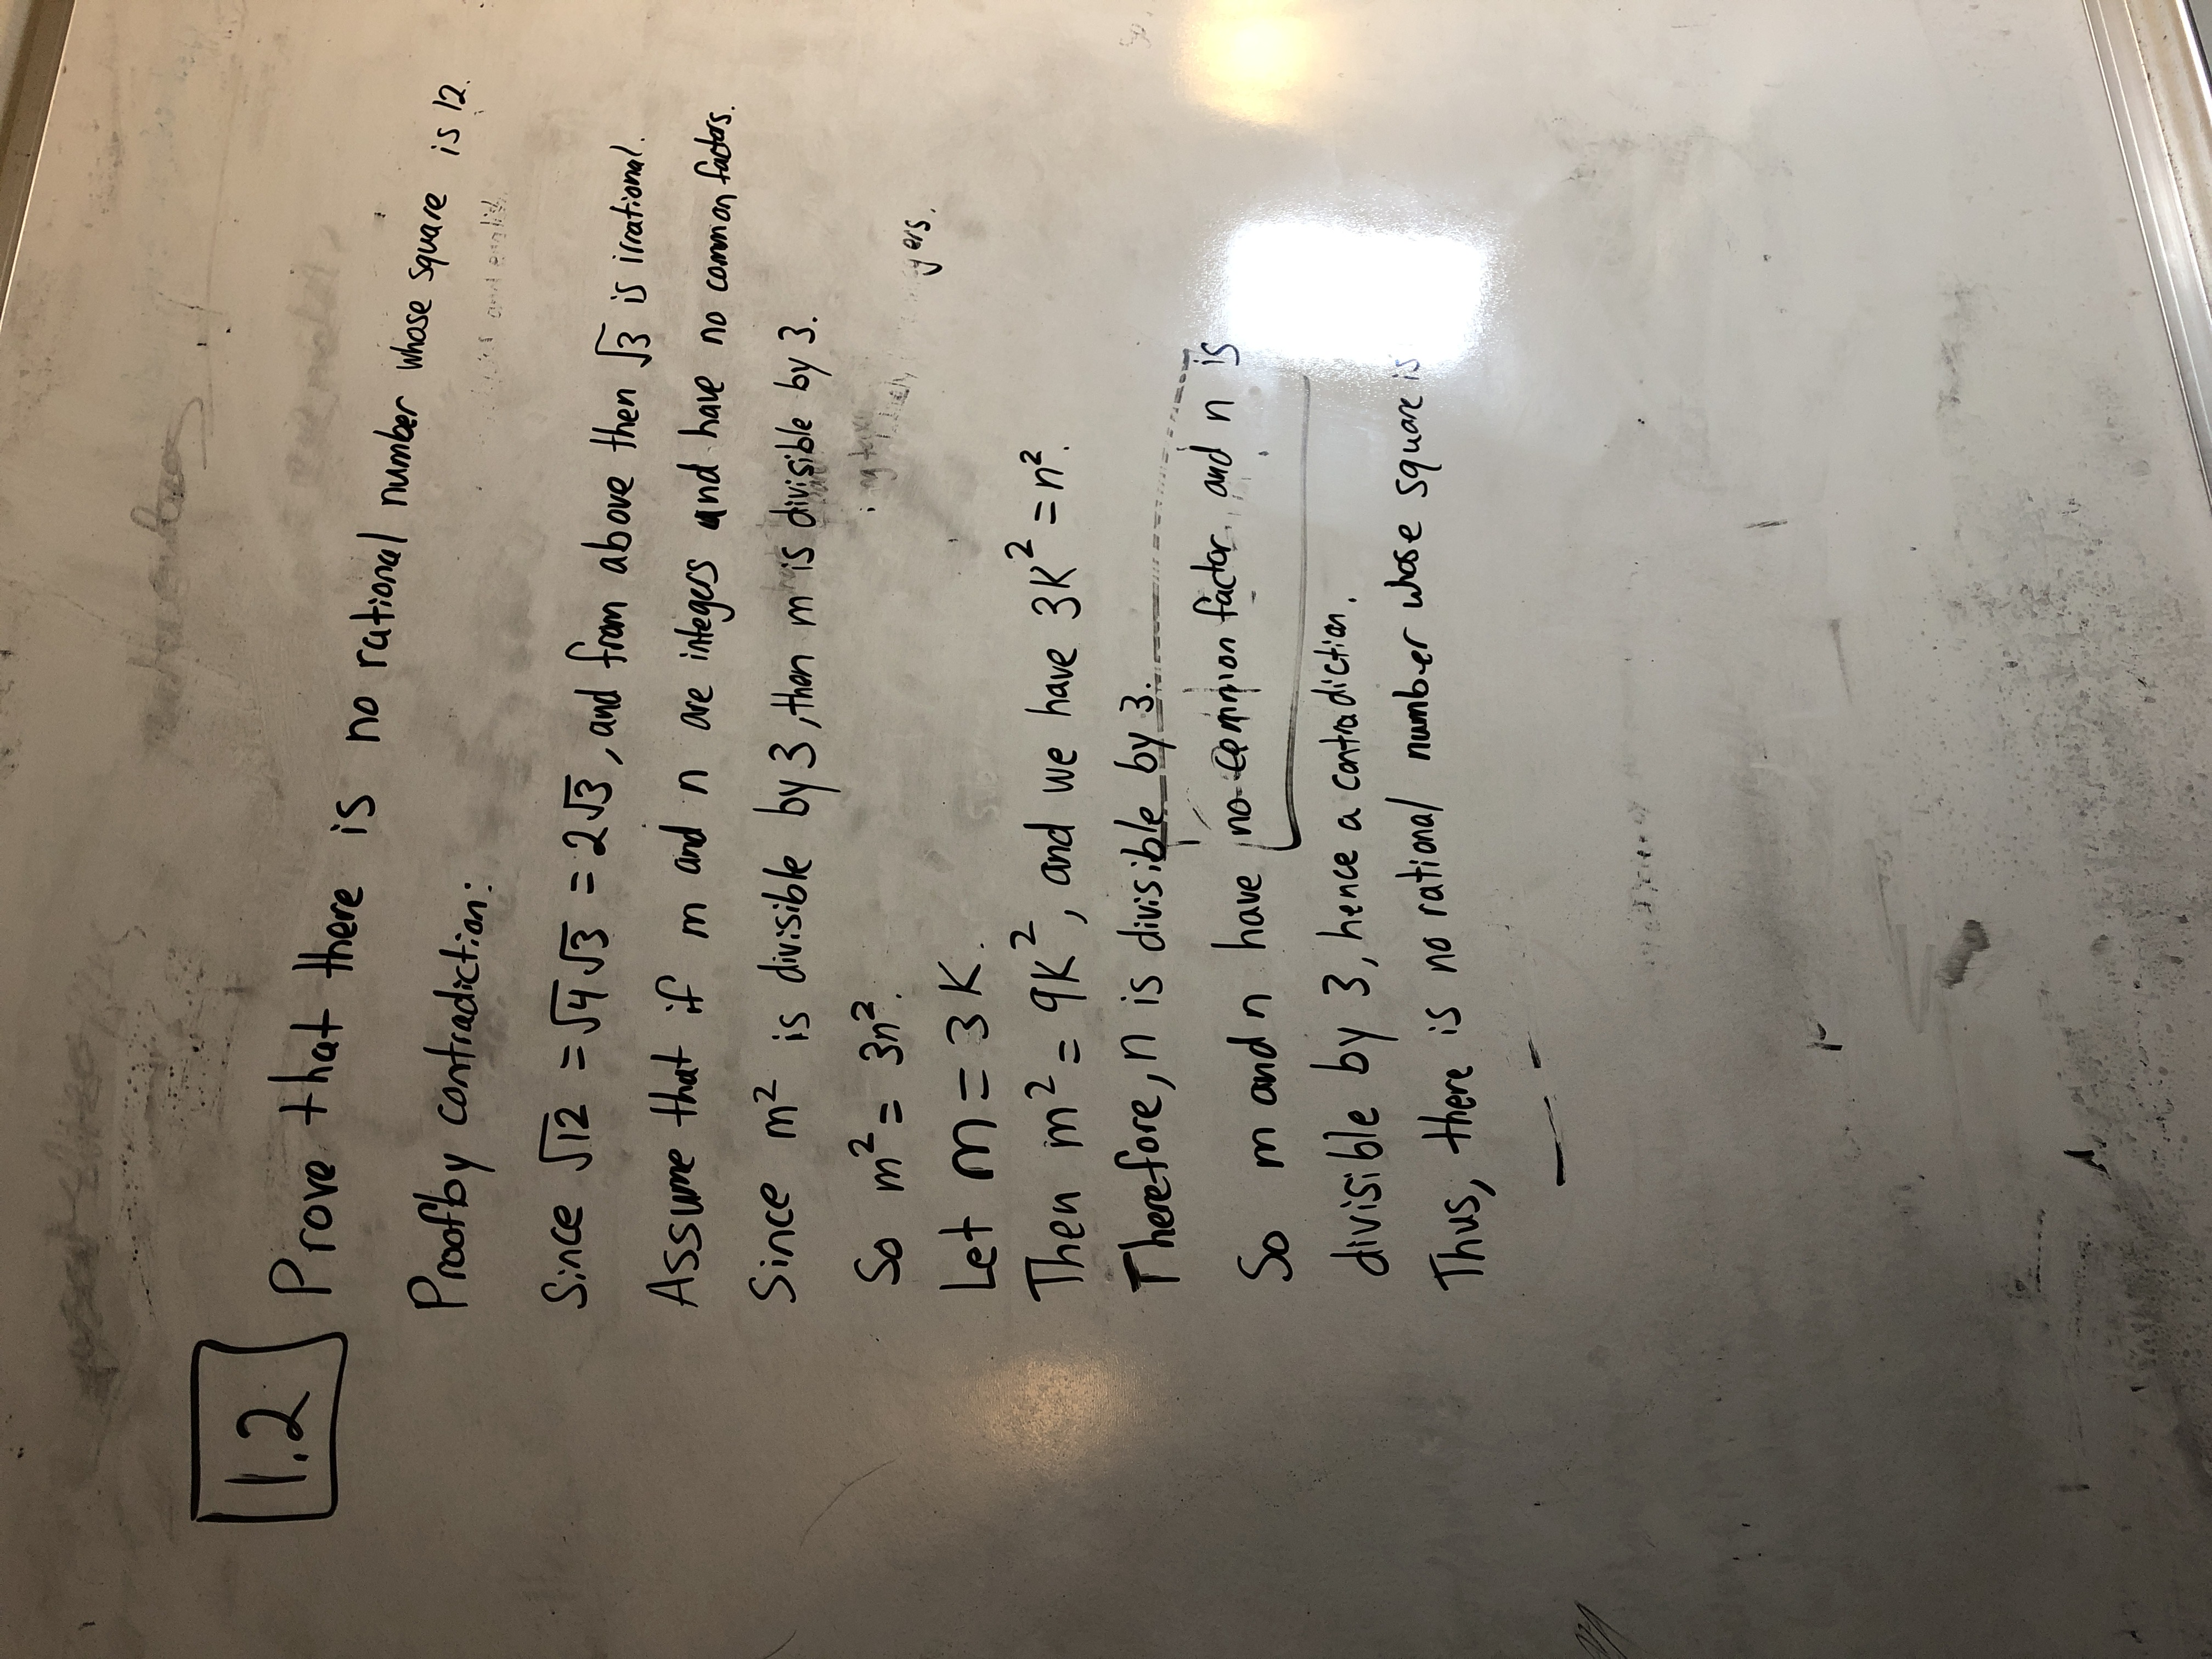
\includegraphics[angle=, origin=c,width=2 in]{Figures/IMG_1077.JPG}
\caption{Placeholder for my proofs} \label{fig:Euler_pic}\end{center}\end{figure} 
Find an example of an interval [a,b] and a function f(x) such that $g(x)=f(x)$ throughout the interval. (3 points). \\
\begin{figure}[h]\begin{center}\includegraphics[angle=, origin=c,width=2 in]{WhiteboardPictures/Exam 2/IMG_1052.JPG}
\caption{Placeholder for my proofs} \label{fig:Euler_pic}\end{center}\end{figure} 
\newpage 
Find an example of an interval $[a,b]$ and a function f(x) such that $g(x) \neq f(x)$ for $x>a.$ (4 points) \\ 

\begin{figure}[h]\begin{center}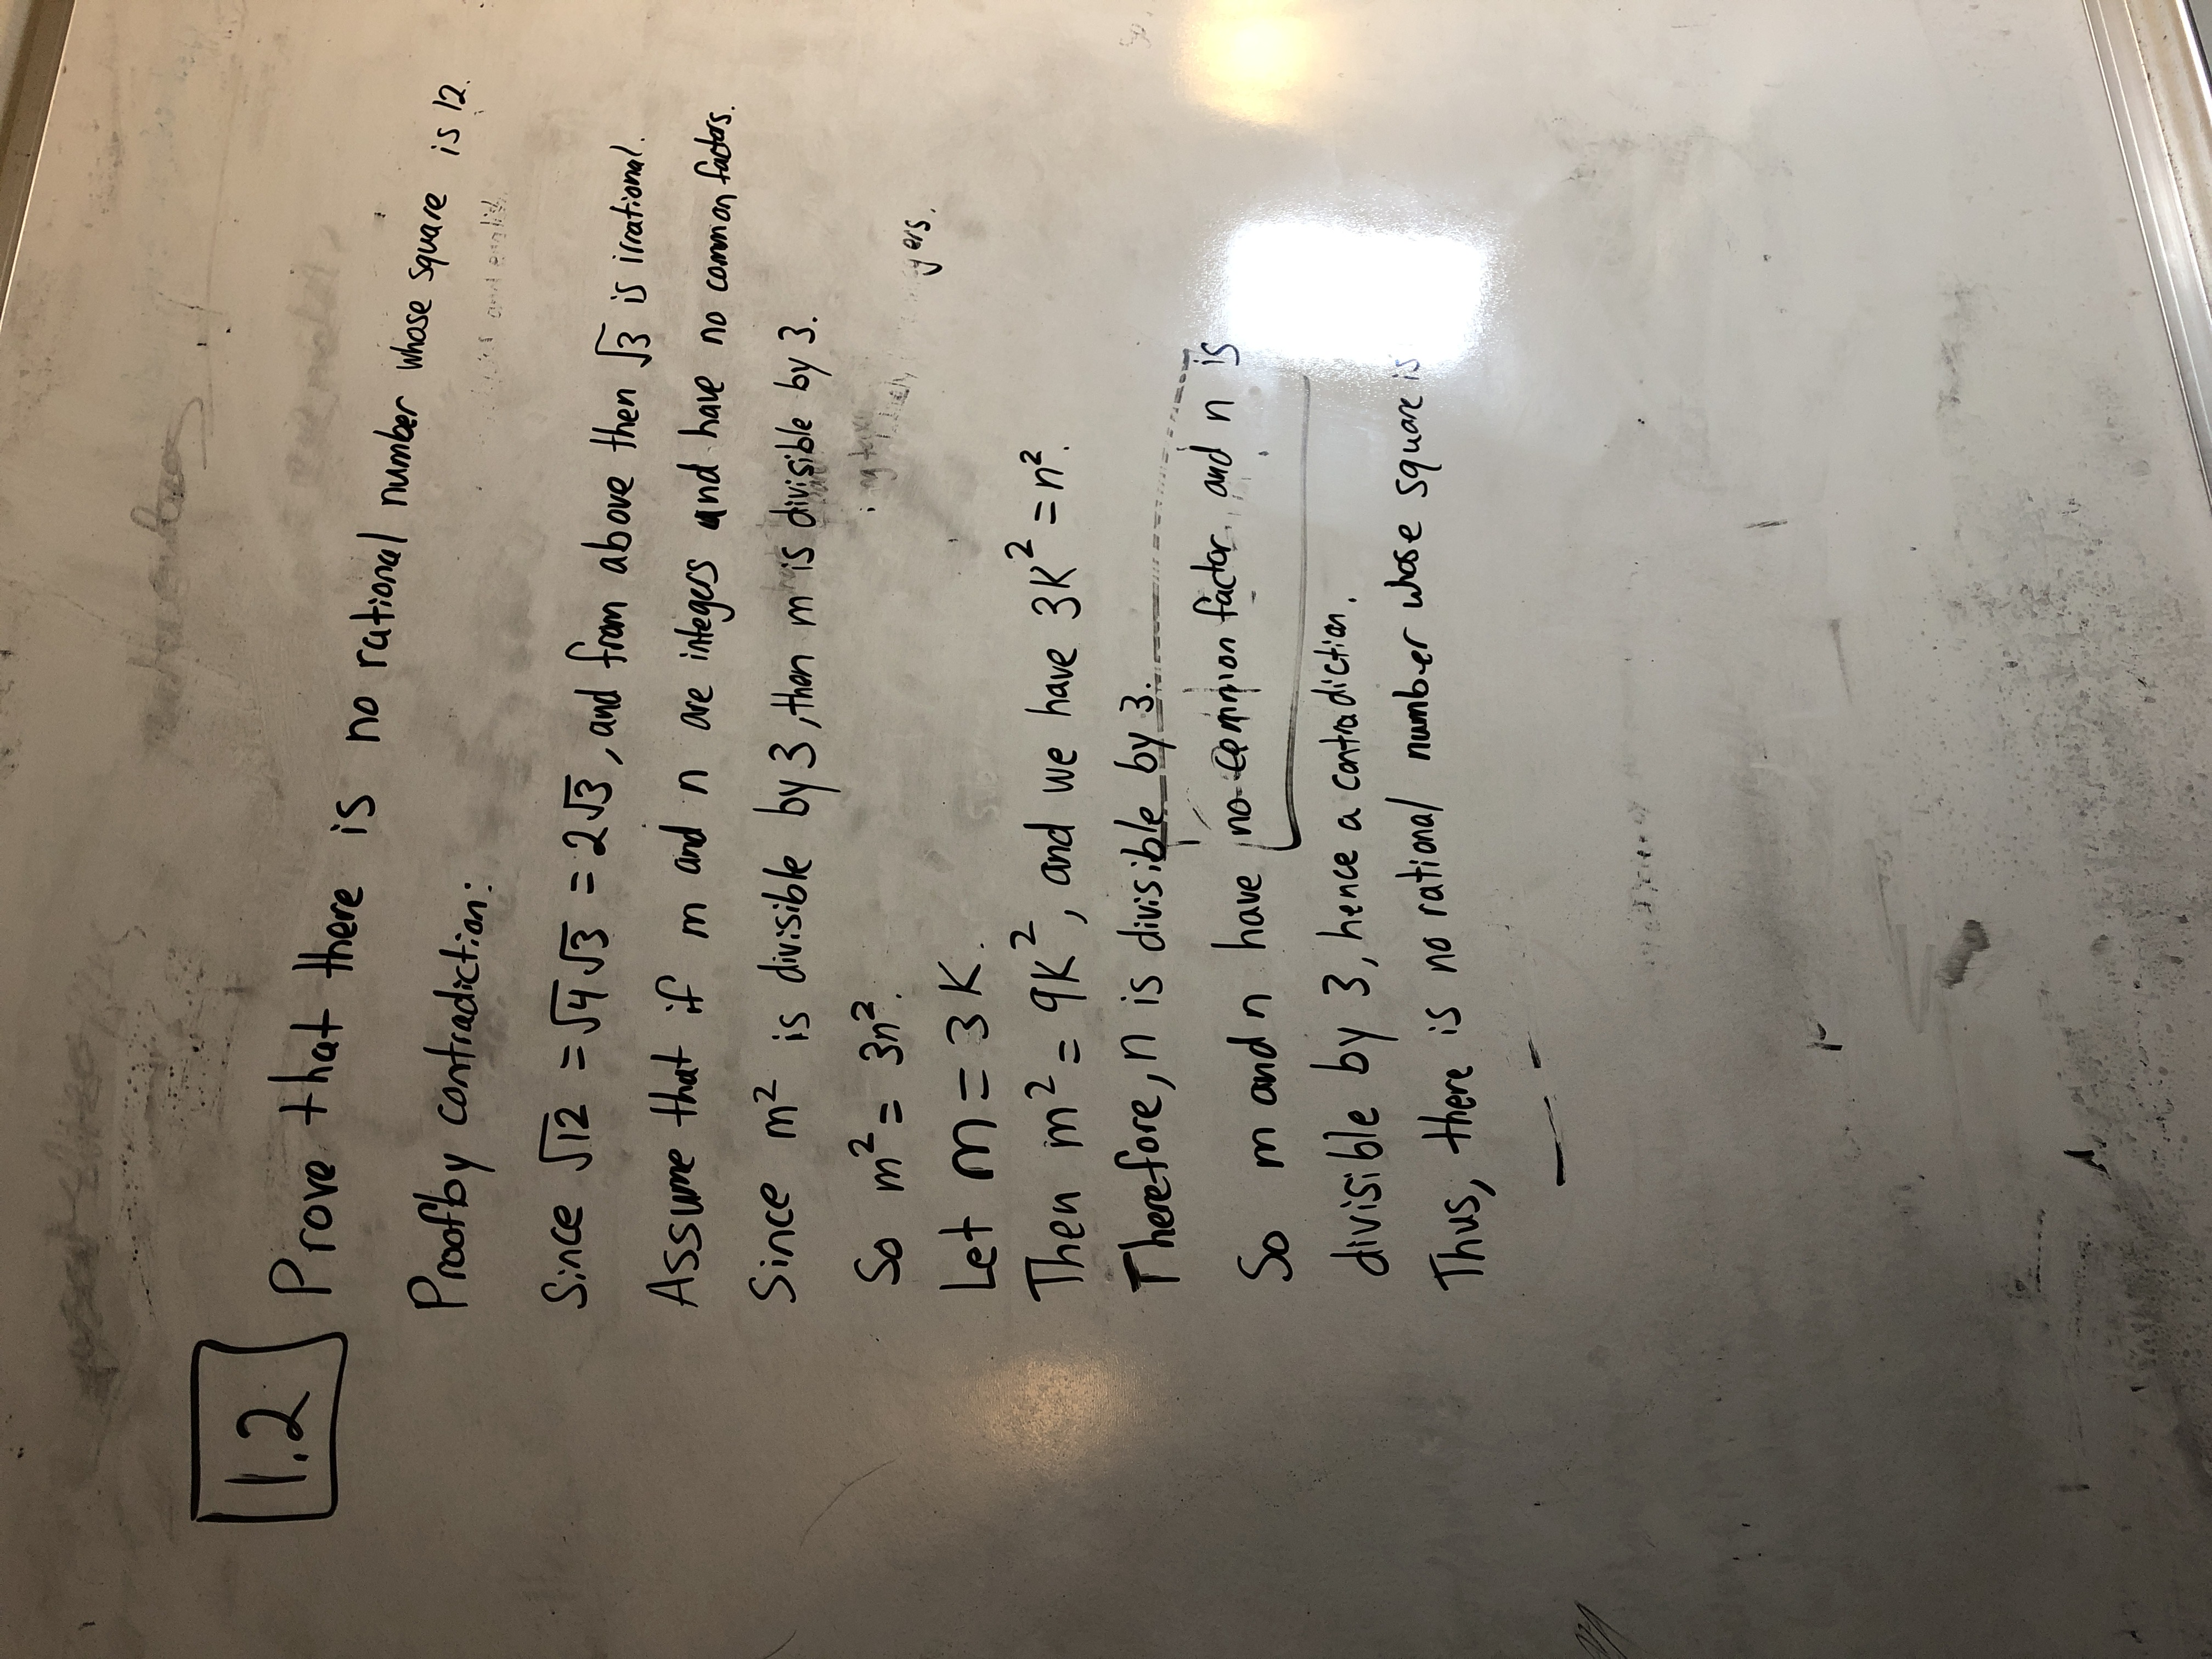
\includegraphics[angle=, origin=c,width=2 in]{Figures/IMG_1077.JPG}
\caption{Placeholder for my proofs} \label{fig:Euler_pic}\end{center}\end{figure} 


Find an example of an interval $[a,b]$ and a function f(x) such that $g(x)=f(x)$ on an open sub-interval whose left endpoint is a, such that $g(x)=f(x)$ on an open sub-interval whose right endpoint is b, and such that $g(x) =\neq f(x)$ on some open sub-interval. Note that you are to find an example of one function with all three of these properties. (4 points) \\ 
\begin{figure}[h]\begin{center}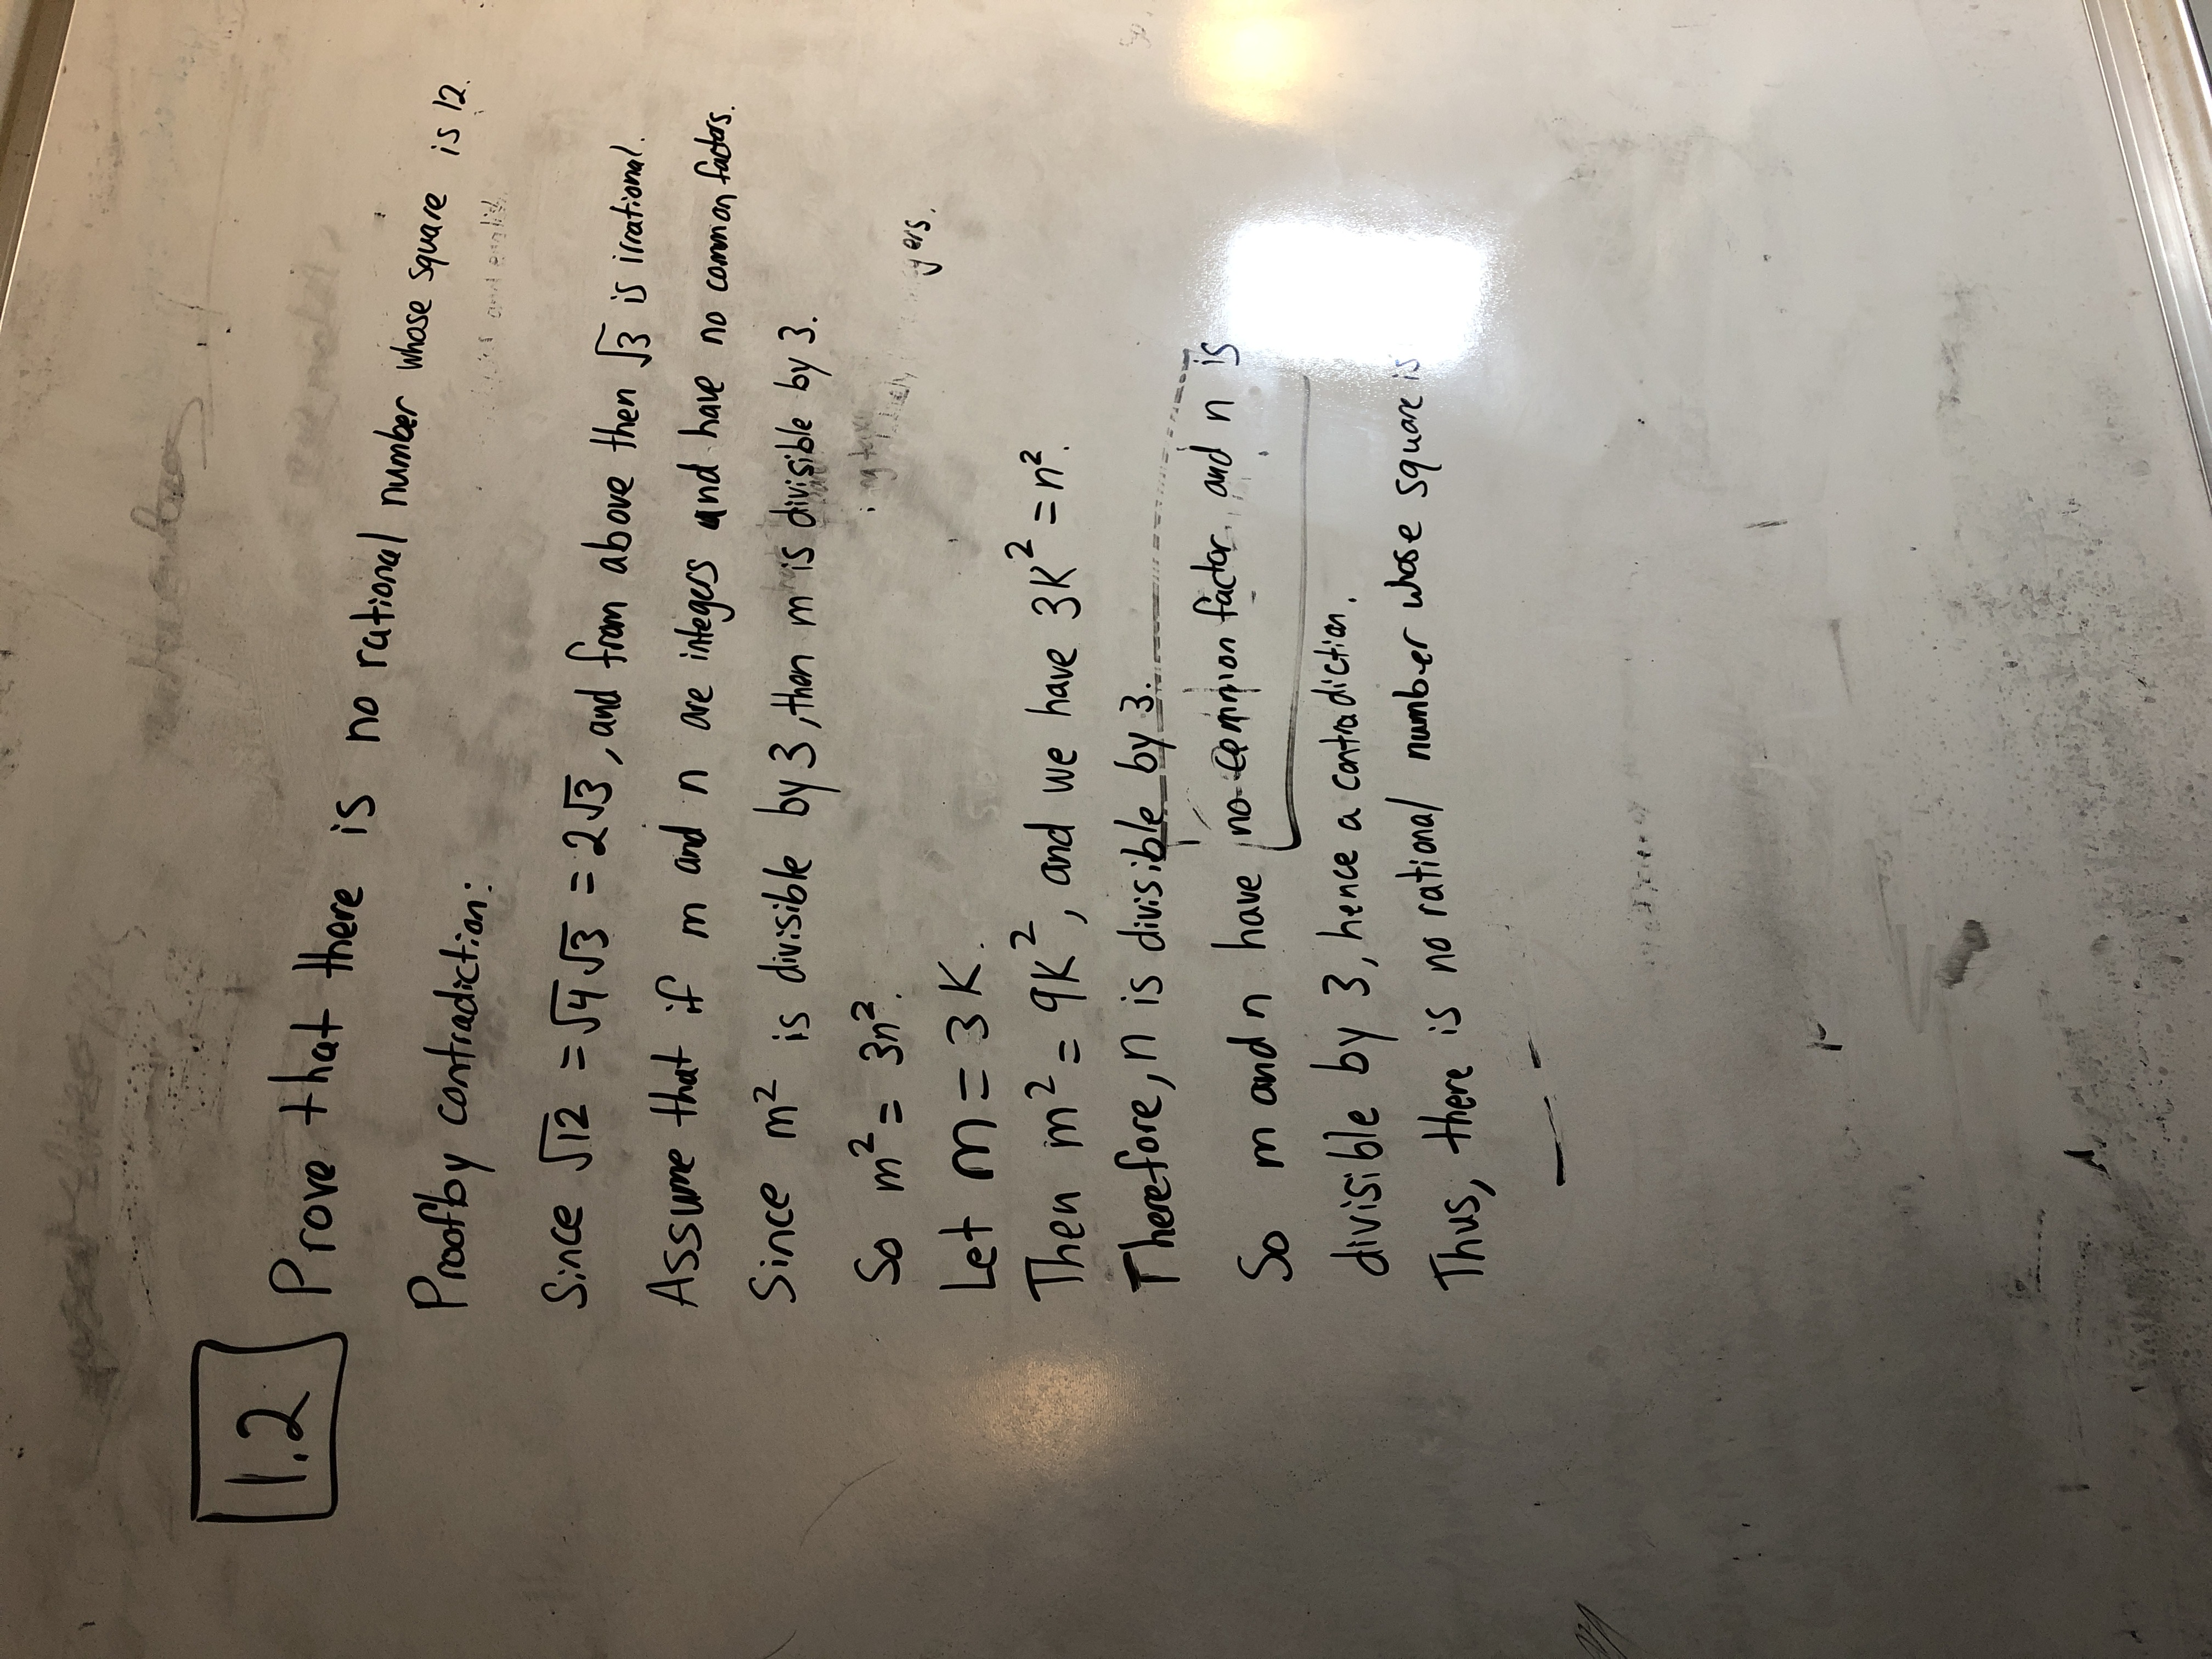
\includegraphics[angle=, origin=c,width=2 in]{Figures/IMG_1077.JPG}
\caption{Placeholder for my proofs} \label{fig:Euler_pic}\end{center}\end{figure} 
\\

\newpage
If f(x) is differentiable, need $g(x)$ be differentiable? Prove your claim. (5 points). \\ 

\begin{figure}[h]\begin{center}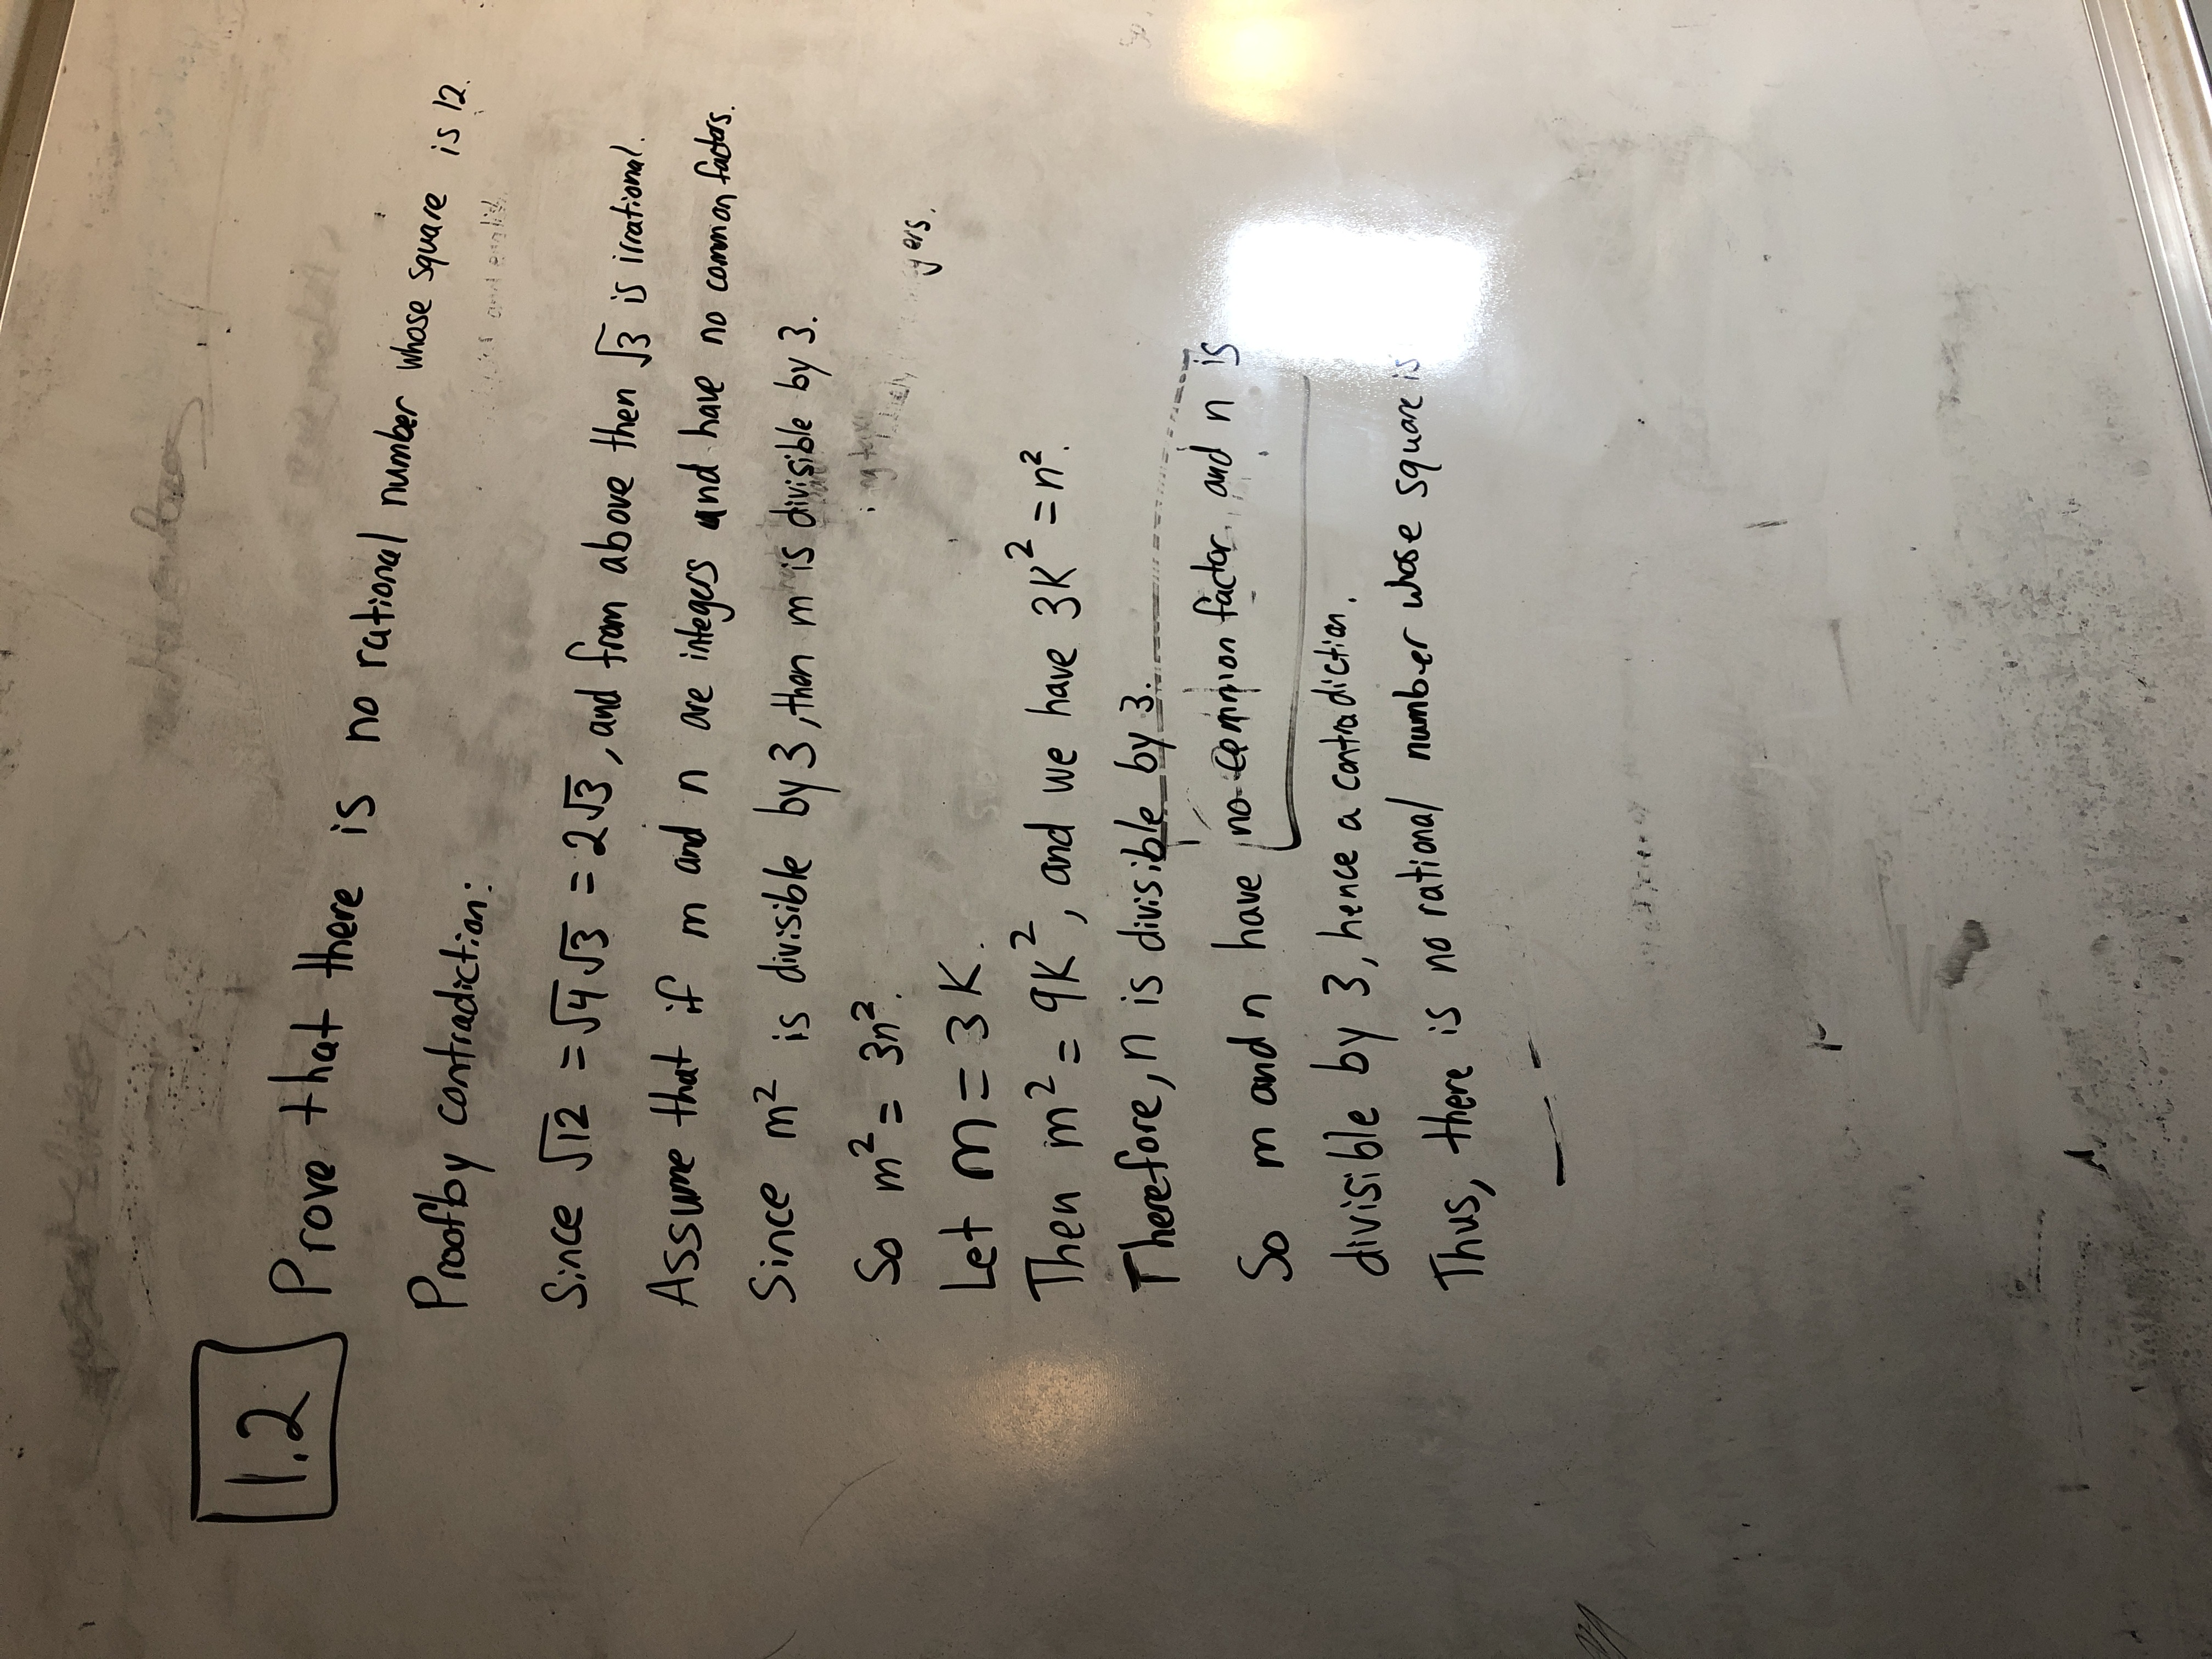
\includegraphics[angle=, origin=c,width=2 in]{Figures/IMG_1077.JPG}
\caption{Placeholder for my proofs} \label{fig:Euler_pic}\end{center}\end{figure} 
\\
\newpage
If f(x) is differentiable, it is possible for g(x) to be differentiable? Prove your claim. (4 points).


\begin{figure}[h]\begin{center}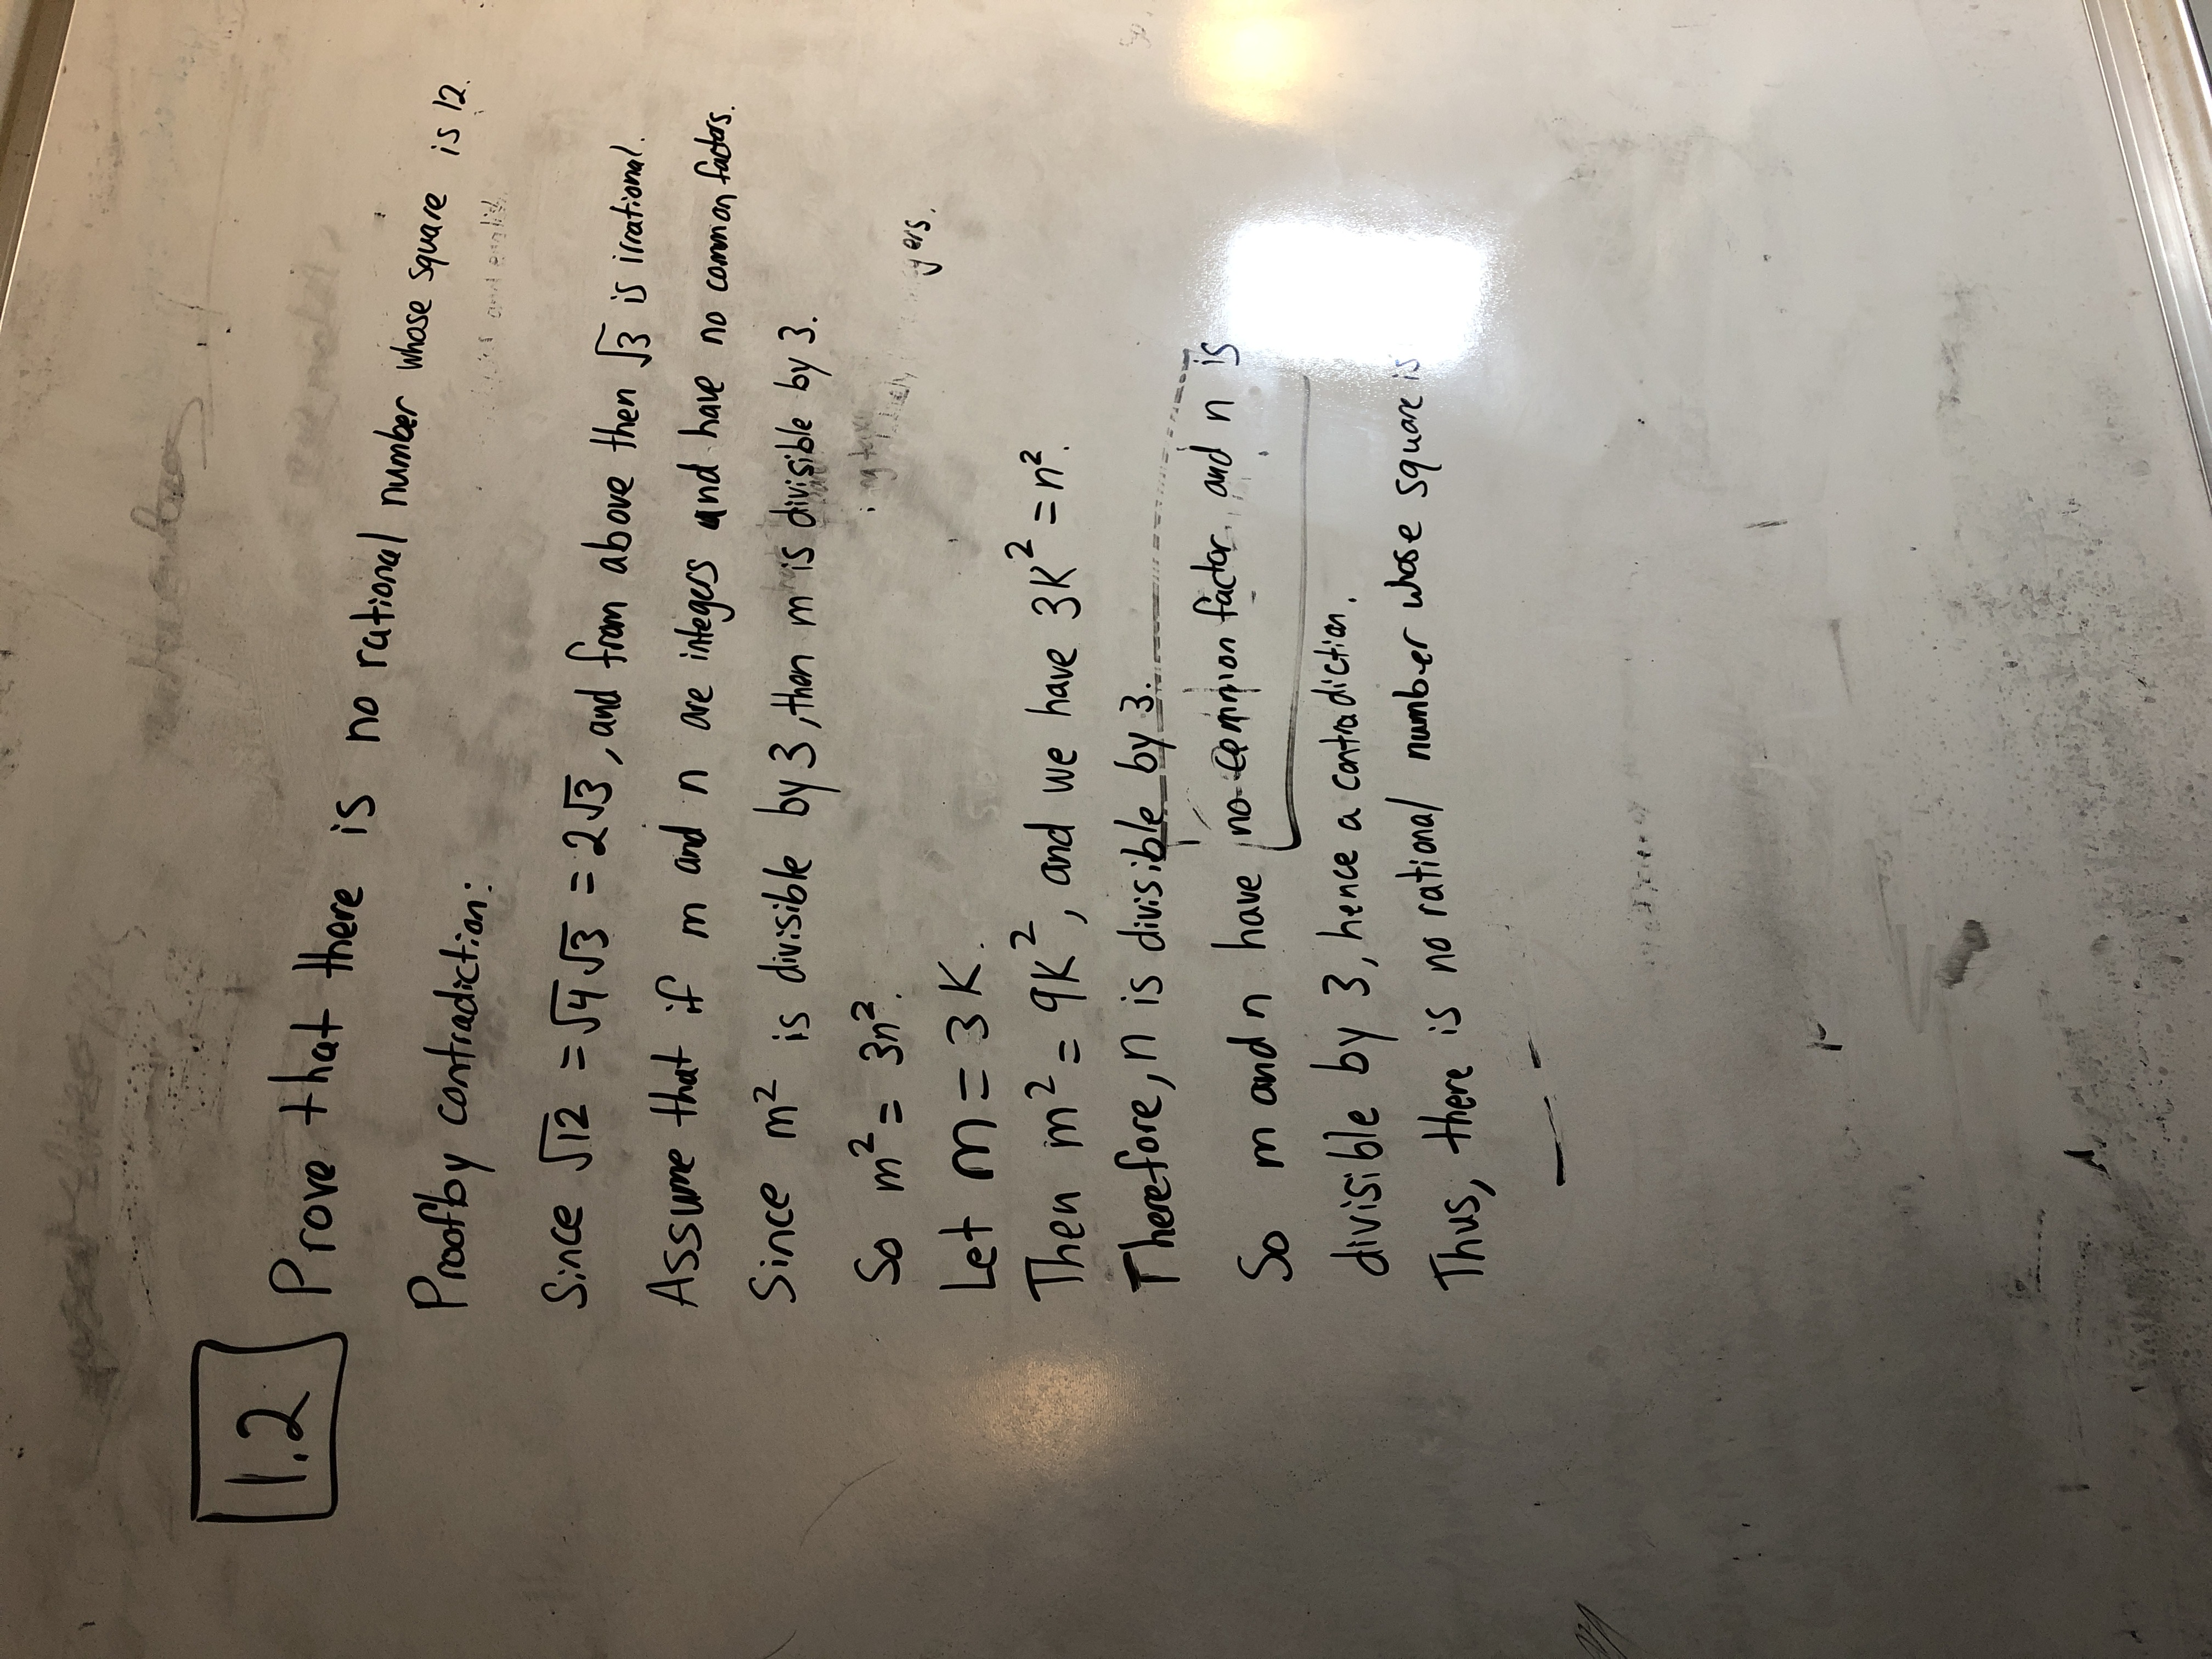
\includegraphics[angle=, origin=c,width=2 in]{Figures/IMG_1077.JPG}
\caption{Placeholder for my proofs} \label{fig:Euler_pic}\end{center}\end{figure} 
\\
\newpage

\section*{7}
(25 points) A function f(x) defined on an interval of $R^1$ is said to be absolutely continuous on that interval if for every $ \epsilon>0 $ there is a $\delta>0$ such that for every collection of disjoint intervals $x_j,y_j) j=1,...,N,$ if $\sum_{j=1}^N y_j -x_j <\delta$ then $\sum_{j=1}^N|f(y_j)-f(x_j)|<\epsilon.$ \\ 
A function f(x) defined on an interval of $R^1$ is said to be Lipschitz on that interval if there is a constant L such that $|f(y)-f(x)| \leq L |y-x|$ for every pair of values x and y in the interval. \\ 






(a) Prove that on a fixed interval every Lipschitz function is absolutely continuous, but that not every absolutely continuous function is Lipschitz.  (5 points) 

\begin{figure}[h]\begin{center}\includegraphics[angle=, origin=c,width=2 in]{WhiteboardPictures/Exam 2/IMG_1052.JPG}
\caption{Placeholder for my proofs} \label{fig:Euler_pic}\end{center}\end{figure} 
\\ 
Let $e>0$ and $\delta= \frac{\epsilon}{M}.$ Then for any collection ${[x_i,y_i}$ of intervals with $\sum |x_i -y_i|<\delta.$ \\ 
Now $\sum |f(x_i)-f(y_i)|<M \sum|x_i-y_i|<e. $ \\
Therefore f is Lipschitz continuous. \\ 
Therefore $\sum|f(x_i)-f(y_i)|<e.$ \\ 

Counter example \\ 
Take $f(x)= \sqrt{x}$ on $[0,k].$ \\ 
$-\sqrt{y} \leq \sqrt{y}.$ \\ 
$\sqrt{x}- \sqrt{y} \leq \sqrt{x} +\sqrt{y}.$ \\ 
$(\sqrt{x}-\sqrt{y})^2 \leq (\sqrt{x}-\sqrt{y})(\sqrt{x}+\sqrt{y})=x-y<\delta.$ \\ 
Therefore $f(x)=f(y)> \sqrt{x}-\sqrt{y}< \sqrt{\delta}= \epsilon.$ \\ 
Choose $\delta=\epsilon^2,$ hence f is absolutely continuous but f(x) =$\frac{1}{2 \sqrt{x}}$ is not bounded. Hence f is not Lipschitz. 

\newpage 
(b) Prove that on a fixed interval every absolutely continuous function is uniformly continuous, but that not every uniformly continuous function is absolutely continuous.  (5 points) 


\begin{figure}[h]\begin{center}\includegraphics[angle=, origin=c,width=2 in]{WhiteboardPictures/Exam 2/IMG_1052.JPG}
\caption{Placeholder for my proofs} \label{fig:Euler_pic}\end{center}\end{figure} 

We have the result that a function satisfying Lipschitz condition is an interval is a uniformly continuous function. \\ 
Hence by (a) an absolutely continuous, uniformly continuous converse is not true. \\ 
Counter example: $f(x)=x^2sin(x)$ on $[0,1]$ \\ 
$f(x)=0$ at x=0. \\


(c)Prove that on a fixed interval every uniformly continuous function is continuous, but that not every continuous function is uniformly continuous.  (5 points) \\ 

\begin{figure}[h]\begin{center}\includegraphics[angle=, origin=c,width=2 in]{WhiteboardPictures/Exam 2/IMG_1052.JPG}
\caption{Placeholder for my proofs} \label{fig:Euler_pic}\end{center}\end{figure} 

Let f: $x \longrightarrow R$ be uniformly continuous then  by definition for any $\epsilon>0$ there exists $\delta>0$ such that $x,y \in X, |x-y|<\delta.$ \\ 
$|f(x)-f(y)<\epsilon.$ \\ 
In particular if we fix $c \in X.$ \\ 
$|x-c|<\delta$ \\ 
$f(x)-f(x)< \epsilon$ for every $c \in X$ f is continuous. \\ 
Converse is not true. \\ 
Counterexample $f(x)=\frac{1}{x}$ in $R^+$ (If we take $x= \frac{1}{n},$ $y=\frac{1}{2}n$ then we can show f is not uniformly continuous.)



Prove that on a fixed interval every differentiable function with bounded derivative is uniformly continuous. (5 points)  

\begin{figure}[h]\begin{center}\includegraphics[angle=, origin=c,width=2 in]{WhiteboardPictures/Exam 2/IMG_1052.JPG}
\caption{Placeholder for my proofs} \label{fig:Euler_pic}\end{center}\end{figure} 

\\ 
Since $f^1$ is bounded then there exists $M>0$ such that $|f(x)|\leq M$ for all x $\in I=[a,b].$ \\ 
Now applying the mean value theorem $f(a)=f(b)=f(\epsilon)(a-b).$ \\ 
In general, $\frac{|f(x)-f(y)|}{|x-y|} \leq M$ \\ 
$|f(x)-f(y)| \leq M|x-y|$ for all x,y $\in I.$ \\ 
So, f is Lipschitz continuous on $I.$ \\ 
F is uniformly continuous. 


\newpage 
Prove that on a fixed interval a differentiable function whose derivative is unbounded may or may not be uniformly continuous. (5 points) 

\begin{figure}[h]\begin{center}\includegraphics[angle=, origin=c,width=2 in]{WhiteboardPictures/Exam 2/IMG_1052.JPG}
\caption{Placeholder for my proofs} \label{fig:Euler_pic}\end{center}\end{figure} 


\section{Unedited: Chapter 4 Baby Rudin}
\section*{1}
Suppose f is a real function defined on $R^1$ which satisfies $lim_{h \longrightarrow 0}[f(x+h)-f(x-h)]=0$ \\ for every $x \in R^1.$ Does this imply that f is continuous? \\ 
Solution: \\ 
No. If x is in $\mathbb{Z}$, then $f(x+h)-f(x-h)= 0$ for all h. \\ 
Yet, if x is not in $\mathbb{Z}$, then $f(x+h)-f(x-h)=0$ for $|h| < min(x-[x],1+[x]-x$. \\ Also,$lim_{h \longrightarrow 0} \frac{f(x+h)-f(x-h)}{h^n}=0$ for every $x \in R_1,$ where n is arbitrary and $>0$, does not imply that f is continuous. \\ 
A counterexample for f being continuous is $f(x)=\frac{1}{x^2}$ when $x\neq 0,$ yet $f(x)=0$ when $x=0.$ Thus, making the f not continuous. 
 \\ 
\section*{2}
If f is a continuous mapping of a metric space X into a metric space Y, prove that $f(\Bar{E}) \subset \Bar{f(E)}$, for every set $E \subset X. (\Bar{E}$ denotes the closure of E.) Show, by an example, that $f(\Bar{E})$ can be a proper subset of $\Bar{f(E)}.$\\ 
Let x $\in \Bar{E}.$ \\ 
We need to show that f(x) $\in \Bar{f(E).}$ \\ 
Let O be any neighborhood of f(x). \\ 
Since f is continuous, $f^{-1}(O)$ contains a neighborhood of x. \\ 
Since O was any neighborhood of $f(x)$, it follows that $f(x) \in \Bar{f(E)}$. \\ 
Consider $f: R ^1 \longrightarrow R^1$ given by $f(x)= \frac{x}{1+x^2}$, and let $E=\Bar{E}=[1, \infty),$ so that $f(E)=f(\Bar{E})= (0, \frac{1}{2}],$ yet $\Bar{f(E)}=[0, \frac{1}{2}].$ \\ 
\section*{3}
Let f be a continuous real function on a metric space X. Let $Z(f)$ (the zero set of f) be the set of all $p \in X$ at which $f(p)=0.$ Prove that $Z(f)$ is closed. \\ 
Notice that Z(f)= $f^{-1}({0})$  which is the inverse image of a closed set. \\Then since ${0}$ is a closed set in the set of the Real numbers then we can use Theorem 4.8's Corollary.\\ Hence Z(f) is closed. 

\\ 
\section*{4}
Let f and g be continuous mappings of a metric space X into a metric space Y, and let E be a dense subset X. Prove that f(E) is dense in f(X). \\ 
If g(p)=f(p) for all $p \in E,$ prove that $g(p)=f(p)$ for all $p \in X.$ \\ 
(In other words, a continuous mapping is determined by its values on a dense subset of its domain.)\\ 
Problem 2's conclusion may be used to prove that $f(E)$ is dense in $f(X).$ \\ 
$f(X)=f(\Bar{E}) \subseteq \Bar{f(E)}.$ \\ 
The function $\phi : X \longrightarrow R^1$ given by $\phi (p) =dy(f(p),g(p))$ is continuous, since $|d_y(f(p),g(p))-d_y(f(q),g(q))| \leq d_y(f(p),f(q))+d_y(g(p),g(q)).$ \\ 
This inequality comes from the triangle inequality, since $d_Y(f(p),g(p) \leq d_Y(f(p),f(q))+d_y(f(q),g(q))+d_y(g(q),g(p)),$ and the inequality holds with p and q swapped. The absolute value $|d_Y(f(p),g(p))-d_Y(f(q),g(q))|$ must be either $d_Y(f(p),g(p))-d_y(f(q),g(q))$ or $d_Y(f(q),g(q))-d_y(f(p),g(p)),$ and the triangle inequality shows that both of these numbers are at most $d_y(f(p),f(q))+d_y(g(p),g(q)).$ and the triangle inequality shows that both of these numbers are at most $d_y(f(p),f(q))+d_y(g(p),g(q)).$ \\ 
Since the zero set of $\phi$ is closed. But the definition $Z(\phi)={p: f(p)=g(p)}$. \\ 
Hence the set of p for which $f(p)=g(p)$ is closed. \\ 
Since by hypothesis it is dense, it must be X. 

\section*{8}
Let f be a real uniformly continuous function on the bounded set E in $R^1.$ Prove that f is bounded on E. \\ 
Show that the conclusion is false if boundedness of E is omitted from the hypothesis. \\ 
Due to f be a real uniformly continuous function on the bounded set E in $R^1$ then there exists a $\delta>0$ such that if $|x-y|<\delta$ and $x,y \in E$ then $|f(x)-f(y)|<1.$ \\ 
Since $|f(x)|-|f(y)|\leq |f(x)-f(y)|$ this implies that $|f(x)|<1+|f(y)|.$\\ 
So $\Bar{E}$ is closed and bounded in $\R$ since E is a bounded set in $\R.$ \\ 
Next, ${B_{\delta}(y)}$ where $y \in E$ is an open cover of $\Bar{E}$ so that there exists a finite subcover ${B_{\delta}(y_{j})}$ for j=1,2,...,n of $\Bar{E}.$ \\ 
This means that for any $x \in E,$ $x \in B_{\delta}(y_i)$ for some i and thus $|f(x)|<1+|f(y_i)|\leq$ max for $1\leq j \leq n {1+|f(y_j)|}$.
Therefore, this proves that f is bounded on E with M=max for $1\leq j \leq n {1+|f(y_j)|}$ bounded. \\ 
The function $f(x)=x$ is uniformly continuous on the entire line, but not bounded. \\ 
%Let $E$ be bounded by $M>0$, so %$|x|\leq M \forall x \in E.$\\ 
%Due to the fact that f is uniformly %continuous, $let \epsilon=1$ then %there exists $\delta>0$ such that %when $|x-y|<\delta$ where $x,y \in E$ %then $|f(x)-f(y)|<\epsilon.$ \\ 

%Let a= inf E and b=sup E, and let %$\delta >0$ be such that %$|f(x)-f(y)|<1$ if $x,y \in E$ and %$|x-y|<\delta$. Now choose a positive %integer N larger than $(b-a)/\delta$, %and consider the N intervals $I_k= %[a+\frac{k-1}{b-a},a+\frac{k}{b-a}],$ %k=1,2,...,N. \\ 
%For each k such that $I_k \cap E \neq %\empty $ let $x_k \in E \cap I_k.$ \\ 
%Then let $M=1 + max{|f(x_k)|}.$ \\ 
%If $x \in E,$ we have $|x-x_k|< %\delta$ for some k, and hence %$|f(x)|<M.$ \\ 
7,9,11,12
\section*{7}
If $E \subset X$ and if f is a function defined on X, the restriction of f to E is the function g whose domain of definition is E, such that g(p) = f(p) for $p \in E.$ \\ 
Define f and g on $R^2$ by $f(0,0)=g(0,0)=0$, \\ 
$f(x,y)= xy^2/ (x^2 +y^6) if (x,y) \neq (0,0).$ Prove that f is bounded on $R^2$ on $R^2,$ that g is unbounded in every neighborhood of $(0,0),$ and that f is not continuous at $(0,0);$ nevertheless, the restrictions of both f and g to every straight line in $R^2$ are continuous! \\ 

f is bounded on $R^2$ since $(|x|-y^2)^2 \leq 0.$ \\ 
Then $x^2-2|x|y^2+y^4 \geq 0.$ \\ 
$x^2+y^4 \geq 2|x|y^2.$\\ 
$\frac{1}{2}\geq |\frac{xy^2}{x^2+y^4}|.$ \\
g is unbounded in every neighborhood of(0,0) because if we let $x_n=\frac{1}{n^3}$ and $y_n=\frac{1}{n}$ then $x_n,y_n) \longrightarrow$ (0,0) and $g(x_n,y_n)=\frac{\frac{1}{n^3}\frac{1}{n^2}}{\frac{1}{n^6}+\frac{1}{n^6}}=\frac{\frac{1}{n^5}}{\frac{2}{n^6}}=\frac{n}{2} \longrightarrow \infty.$ \\ 
This is because $(x_n,y_n) \longrightarrow (0,0)$ implies that for any neighborhood U of (0,0), there is some $N \in \N$ such that $x_n,y_n) \in U for n \geq N,$ and $g(x_n,y_n)$ gets arbitrarily large. Next, we show f is not continuous at $p=(0,0)$ simply by using Theorems 4.2 and Theorem 4.6 to say f is continuous at p. \\ 
Then $lim_{x \longrightarrow p}f(x)=f(p).$ \\ 
$f(p_n)\longrightarrowf(p)$ for every sequence $p_n \longrightarrow p.$ \\ 
So to show f is not continuous, we only need to find one sequence $p_n \longrightarrow p $ such that $f(p_n)$ does not $\longrightarrow f(p).$ \\ 
Let $x_n=\frac{1}{n^2}$ and $y_n=\frac{1}{n}$ and put $p_n=(x_n,y_n),$ so that $p_n \longrightarrow p$= (0,0). \\ 
Next $f(p_n)=f(x_n,y_n)=\frac{\frac{1}{n^2}\frac{1}{n^2}}{\frac{1}{n^4}+\frac{1}{n^4}}=\frac{\frac{1}{n^4}}{\frac{2}{n^4}}=\frac{1}{2}\neq 0=f(0,0)=f(p),$ so f is not continuous at $(0,0).$ \\ 
Lastly, we show that the restriction of f and g to straight lines in $R^2$ are continuous functions. \\ 
f and g are continuous on $R^2\ {(0,0)}$ because they are composed of addition, multiplication, and division with a denominator that is nonzero on $R^2\ {(0,0)}.$ \\ 
Therefore f and g restricted to any line that does not go through (0, 0) are already continuous. What we need to
check is that they are continuous at (0, 0) for any line going through (0, 0). There are two lines of
this form: y = mx and x = 0. Along the line x = 0, f and g are constantly 0, so they are continuous.
Along the line y = mx, for x $\new$ 0, we have 
$f(x,mx)=\frac{x(mx)^2}{x^2+(mx)^4}=\frac{m^2x}{1+m^4x^2} \longrightarrow= f(0,0)$ as $x \longrightarrow 0,$ and $g(x,mx)=\frac{x(mx)^2}{x^2+(mx)^6}=\frac{m^2x}{1+m^6x^2} \longrightarrow 0 =g(0,0)$ as $x \longrightarrow 0,$ so f and g are continuous at $(0,0)$ when restricted to straight lines. 


%    Since $x^2+y^4 \geq 2xy^2$, $f(x,y) \leq 2$ for all $(x,y) \in R^2$.
%    That is, $f$ is bounded by 2.  Next, select
%\[
%        (x_n,y_n) = (\frac{1}{n^3},\frac{1}{n}).
%\]
%    $(x_n,y_n) \rightarrow (0,0)$ as $n \rightarrow \infty$, and
%    $g(x_n,y_n) = n/2 \rightarrow \infty$ as $n \rightarrow \infty$,
%    that is, $g(x,y)$ is unbounded in every neighborhood of $(0,0)$ by
%    choosing large enough $n$.

%    Next, select
%\[
%        (x_n,y_n) = (\frac{1}{n^2},\frac{1}{n}).
%\]
%    $(x_n,y_n) \rightarrow (0,0)$ as $n \rightarrow \infty$, and
%    $f(x_n,y_n) = 1/2$ for all $n$.  Thus,
%\[
        %\lim_{n \rightarrow \infty} f(x_n,y_n) = \frac{1}{2} \neq 0 = %f(0,0).
%\]
    %for some sequence $\{(x_n,y_n)\}$ in $R^2$.  Thus, $f$ is not
    %continuous at $(0,0)$.

    %Finally, we consider two cases of straight lines in $R^2$: (1) $x=c$
    %and (2) $y=ax+b$.  (equation of straight lines).

    %(1) $x = c$:
    %If $c \neq 0$, $f(x,y) = cy^2/(c^2 + y^4)$ and $g(x,y) = cy^2/(c^2 + %y^6)$
    %are continuous since $cy^2$, $c^2 + y^4$, and $c^2 + y^6$ are
    %continuous on $R^1$ respect to $y$, and $c^2 + y^4$, $c^2 + y^6$
    %are nonzero.  If $c = 0$, then $f(x,y) = g(x,y) = 0$, and it is
    %continuous trivially.

   % (2) $y=ax+b$:
    %If $b \neq 0$, then this line dose not pass $(0,0)$.  Then $f(x,y)
    %= x(ax+b)^2/(x^2+(ax+b)^4)$ and $g(x,y) = x(ax+b)^2/(x^2+(ax+b)^6)$.
    %By previous method we conclude that $f(x,y)$ and $g(x,y)$ are
    %continuous.  If $b = 0$, then $f(x,y) = 0$ if $(x,y) = (0,0)$;
    %$f(x,y) = a^2 x/(1 + a^4 x^2)$, and $g(x,y) = 0$ if $(x,y) = (0,0)$;
    %$g(x,y) = a^2 x/(1 + a^6 x^4)$.  Thus, $f(x,y) \rightarrow 0/1 = 0 =
    %f(0,0)$ and $g(x,y) \rightarrow 0/1 = 0 = f(0,0)$ as $x \rightarrow %0$.
 %   Thus, $f$ and $g$ are continuous.
%    Both of two cases implies that the restriction of both $f$ and $g$
%    to every straight line in $R^2$ are continuous. \\
%The fact that $f(x,y)| \leq \frac{1}{2}$ is an easy consequence of the inequality $(x-y^2)^2 \geq 0.$ \\ 
%The fact that $lim_{y \longrightarrow0} g(y^3,y) = lim_{y \longrightarrow 0} \frac{y^5}{2y^6}= lim_{y \longrightarrow 0} \frac{1}{2y}= \infty$ shows that g is unbounded on every neighborhood of infinity. \\ 
%The fact that $lim_{y \longrightarrow 0} f(y^2,y)= lim_{y \longrightarrow 0} \frac{y^4}{2y^4}=\frac{1}{2}$ shows that f is not continuous at (0,0). \\ 
%Since f and g are continuous except at $(0,0),$ it is obvious that their restrictions to any line that does not pass through (0,0) are continuous. Now a line that does pass through (0,0) has an equation that is either x=0 or y= ax for some a. \\ 
%Both f and g are constantly 0 on the first of these, and on the second we have $f(x,ax)=a^2x^3/(x^2+a^4x^4)=a^2x/(1+a^4x^2), while g(x,ax)=a^2x^3/(x^2+a^6x^6)=a^2x/(1+a^6x^4).$ Both of the latter are obviously continuous function. 

\section*{9}
Show that the requirement in the definition of uniform continuity can be rephrased as follows, in terms of diameters of sets: To every $ \epsilon >0$ there exists a $\delta >0$ such that $diam f(E)< \epsilon$ for all $E \subset X$ with diam $E< \delta. $\\ 
 \\ 
Suppose f is uniformly continuous and $ \epsilon >0$ is given. \\ 
Choose any positive number $\alpha$ smaller than $\epsilon.$ Then there exists $\delta >0$ such that $d_y(f(x),f(u))<\alpha$ if $d_x(x,u)<\delta.$ \\ 
Hence if E is any set of diameter less than $\delta$ and x and u are any two points in E we have $d_y(f(x),f(u))< \alpha,$ so that diam $f(E) \leq \alpha < \epsilon.$ \\ 
Conversely if f satisfies the condition stated in the problem, it is obvious that for any $\epsilon >0$ there exists $\delta >0$ such that $d_Y(f(x),f(u))<\epsilon$ whenever $d_X(x,u)< \delta.$ (Choose $\delta>0$ corresponding to $\epsilon$ in the condition of the problem and then let E be the two-point set {x,u}.)\\ 
\section*{11}
Suppose f is a uniformly continuous mapping of a metric space X into a metric space Y and prove that ${f(x_n)}$ is a Cauchy sequence in Y for every Cauchy sequence ${x_n}$ in X. Use this result to give an alternative proof of the theorem stated in exercise 13. \\ 
Solution: \\ 
Suppose ${x_n}$ is a Cauchy sequence in X. \\ 
Let $\epsilon >0$ be given. \\ 
Let $\delta >0$ be such that $d_Y(f(x),f(u))<\epsilon$ if $d_X(x,u)<\delta.$\\ 
Then choose N so that $d_X(x_n,x_m)< \delta$ if n,$m >N$. \\ 
Obviously $d_Y(f(x_n),f(x_m))<\epsilon$ if m,n >N, showing that ${f(x_n)}$ is a Cauchy sequence. \\ 
Now let f be a uniformly continuous function defined on a dense subset E of X, mapping E into a complete metric space Y( for example, Y could be the real numbers). To prove that f has a unique continuous extension to all of X, proceed as follows. For each $x \in X \E$ let ${x_n}$ be a sequence of points in E converging to x. \\ 
Define f(x) to be the limit of the Cauchy sequence ${f(x_n)}.$ \\ 
This definition is unambiguous; for if ${u_n}$ also converges to x, then the sequence ${y_n}$ defined by $y_n= x_{n/2}$ if n is even, \\ $u_{(n+1)/2}$ if n is odd, \\ 
also converges to x. \\ 
Hence ${f(y_n)}$ is a Cauchy sequence in Y, and so all subsequences of ${f(y_n)}$ is a Cauchy sequence in Y, and so all  subsequences of ${f(y_n)}$ converge to the same limit. In particular ${f(x_n)}$ and ${f(u_n)}$ both converge to the same value. \\ 
The extended function is also uniformly continuous. For if $ \epsilon >0,$ let $\delta >0$ be such that $d_Y(f(x),f(u))<\\frac{\epsilon}{3}$ if $x,u \in E$ and $d_X(x,u)<\delta.$ \\ 
Then if $x \in E, u \in X\E$ and $d_x(x,u)< \delta,$ choose $v \in E$ with $d_X(v,u)<\delta-d_X(x,u)$ and $d_Y(f(v),(f(u))< \frac{\epsilon}{3}$ (this is possible because of the definition of f(u)). We then have $d_X(x,v) \leq d_x(x,u)+d_X(u,v)< \delta,$ and so \\ 
$d_Y(f(x),f(u)) \leq d_Y(f(x),f(v))+d_Y(f(v),f(u))< \frac{2 \epsilon}{3}< \epsilon.$\\ 
Similarly, if $x \in X \E, u \in X\E,$ and $d_X(x,u)< \delta,$ choose v,w $\in E$ with $d_X(v,u)<\frac{1}{2}(\delta-d_X(x,u)),d_X(x,w)<\frac{1}{2}(\delta-d_X(x,u)),d_Y(f(v),f(u))<\frac{\epsilon}{3},$ and $d_Y(f(w),f(x))<\frac{\epsilon}{3}.$ We then have $d_X(v,w) \leq d_X(v,u)+d_X(u,x)+d_X(x,w)< \delta$ and hence $d_Y(f(x),f(u)) \leq d_Y(f(x),f(w))+d_Y(f(w),f(v))+d_Y(f(v),f(u))< \epsilon.$ \\ 
The uniqueness of this extension follows from exercise 4 above. 

\section*{12}
A uniformly continuous function of a uniformly continuous function is uniformly continuous. \\ 
State this more precisely and prove it. \\ 
Let $f: X \longrightarrow Y$ and $g: Y \longrightarrow Z$ be uniformly continuous. \\ 
Then $g \circ f : X \longrightarrow Z$ is uniformly continuous, where $g \circ f(x)=g(f(x))$ for all $x \in X.$ \\ 
To prove this fact, let $ \epsilon>0$ be given. \\ 
Then since g is uniformly continuous, there exists $ \nu >0$ such that $d_Z(g(u),g(v))< \epsilon$ if $d_Y(u,v)< \nu.$ \\ 
Since f is uniformly continuous, there exists $\delta >0$ such that $d_Y(f(x),f(y))< \nu$ if $d_X(x,y) < \delta.$ \\ 
It is then obvious that $d_Z(g(f(x)),g(f(y)))< \epsilon$ if $d_X(x,y)< \delta,$ so that $g \circ f$ is uniformly continuous. 



\section{Chapter 5 Baby Rudin: Unedited}


\subsection{1,2,3,4}

\subsubsection{Prove that f is constant as functions absolute value}
\subsubsection*{Problem 5.1}

Let f be defined for all real x, and suppose that $|f(x)-f(y)|\leq (x-y)^2$ for all real x and y. Prove that f is constant. \\ 
Proof: \\ 
Dividing by x-y, and letting $x \rightarrow y,$ and letting $x \rightarrow y,$ we find that $f'(y)=0$ for all y. Hence f is constant. 

\subsubsection*{Prove g is differentiable}
Suppose $f'(x)>0$ in (a,b). Prove that f is strictly increasing in $(a,b),$ and let g be its inverse function. Prove that g is differentiable, and that $g'(f(x))=\frac{1}{f'(x)} (a<x<b).$\\ 
Proof: \\ 
For any c,d, with a<c<d<b there exists a point $p \in (c,d),$ such that $f(d)-f(c)=f'(p)(d-c)>0.$\\ 
Hence $f(c)<f(d).$\\
Now referring to Theorem 4.17... \\

Baby Rudin explains in his rigorous math way, that the inverse function g is continuous. (Its restriction to each closed subinterval [c,d] is continuous, and that is sufficient.) \\ 
Now observe that if $f(x)=y$ and $f(x+h)=y+k,$ \\ 
we have $\frac{g(y+k)-g(y)}{k}-\frac{1}{f'(x)}=\frac{1}{\frac{f(x+h)-f(x)}{h}}-\frac{1}{f'(x)}.$\\ 
Since we know lim $\frac{1}{\phi(t)}=\frac{1}{lim \phi(t)}$ provided lim $\phi(t)\neq 0,$ it follows that for any $\epsilon >0$ there exists $\nu >0$ such that $|\frac{1}{\frac{f(x+h)-f(x)}{h}}-\frac{1}{f'(x)}|<\epsilon$ if $0<|h|<\nu.$ \\ 
Since $h=g(y+k)-g(y),$ there exists $\delta >0$ such that $0<|h|< \nu $ if $0<|k|<\delta.$ \\ 
The proof is now complete. \subsubsection*{Problem 5.3: Unedited }
Suppose g is a real function on $R^1$ with bounded derivative (say $|g'|\leq M).$ Fix $\epsilon >0,$ and define $f(x)=x+ \epsilon g(x).$ Prove that f is one-to-one if $\epsilon$ is small enough. (A set of admissible values of $\epsilon$ can be determined which depends only on M. \\ 

Proof: \\ 
If $0< \epsilon < \frac{1}{M},$ we certainly have \\ 
$f'(x) \geq 1 - \epsilon M >0,$ and this implies that f(x) is one-to- one, by the preceding problem. \\ 


\subsection*{Baby Rudin: Problem 5.4: Unedited}
If $C_{0}+\frac{C_{1}}{2}+\dots +\frac{C_{n-1}}{n}+\frac{C_n}{n+1}=0$ where $C_0, \dots, C_n$ are real constants, prove that the equation $C_{0}+C_{1}x$+ $\dots + C_{n-1}x^{n-1}+C_{n}x^{n}=0$ has at least one real root between 0 and 1. \\ 
Proof: \\ 
Consider the polynomial \\ 
$p(x)=C_{0}x+\frac{C_1}{2}x^2+\dots \frac{c_{n-1}}{n}x^n+ \frac{C_{n}}{n+1}x^{n+1}$\\ 
whose derivative is $p'(x)=C_{0}+C_{1}x+\dots +C_{n-1}x^{n-1}+C_{n}x^{n}.$\\
It is obvious that $p(0)=0,$ and that the hypothesis of the problem is that $p(1)=0$. Hence Rolle's theorem implies that $p'(x)=0$ for some x between 0 and 1. 


\section{}
\chapter{Tyler and Paulina you are stupid if you think I only know differential...I passed that level 7 years ago}

The novice level is a magnet. The amateur level is the Maxwell's field equations. 
\section[What my Optics Studies have been]{Section with an Unnecessarily Long Title}

Every good story begins with a twist. Let's test it out and see how it 

\subsection{What my Optics interests are in}

Every good story begins with a twist. Let's test it out and see how it 

\subsubsection{Subsubsections, the final formatted heading}

Every good story begins with a twist. Let's test it out and see how it goes. Beginning to ending, just spin 

\section{What I have learned along the way}

Every good story begins with a twist. Let's test it out and see how it goes. Beginning to ending, just spin 
\chapter{Started with Optics now we're here...I went to the dark side}

So I am very anxious and I want to type out everything that I need out of my brain in some sort of dissertation form because I am so anxious with UM just my family and my friends in general based on the fact that they are supportive but very doubtful of me so I mean like they're not doubtful but anytime I actually express the extreme version of what my dreams are I need to make sure that it goes through uhm and they would want me to relax or like being like oh just like it's gonna be OK just take a bath get some rest and I'm just like no my timeline is my timeline I'm sorry in advance that I'm not here to have coffee with you and I'm not here to go to your wedding that was not part of my plan my dreams are a PhD in physics I'm sorry if that's bad but this is how it's going right now in the middle of a pandemic so anyways I'm so far what I've been doing is uhm I transferred to RIT up at some point in my life and and I was doing optics UM ever since 2014 and I got my scholarship I got the cheaper tuition and everything and so while I was concurrently taking the institutional specific courses that I felt were not up at a high enough caliber for me I was teaching myself for a analysis and reading every research paper on optics and bioptics I mean polarization theory and then I was also doing research in astrophysics in the meantime so now I am almost done with the coursework for that on and I just am so anxious because I end up interacting with someone who did not transfer or did not have the same path as me because I worked in industry I made sure to do all these different things to make sure that I was skilled like I learn data science I learned this is that I learned in metal hydrodynamics in the general relativistic sense I carried on the textbook Carol and maybe rooting around everywhere and that is the truth like I listen to YouTube lectures while I fell asleep UM and I really did not have a social life uhm and I know that's surprising because of how I look up but that is the truth of the matter I actually spent time on this and I want to be compensated for it uhm so a man I want to be respected for it with the other men in my field but that's a whole another story I need to figure all of this out because a lot of times like I'm I'm reading or watching like something in terms of like OK like tomography like most of the time like I'm playing like the Russian roulette of like some occupied journal like I always say whatever you wanna call it it's up but it's been 10 like years of that up and so I've just been learning about like diffraction patterns and all of that so it's amazing how much I'm finally understanding all of that and I want to like continue and push forward with that but I do need my prosthetic brain for that kind of work up and I feel like my time is running out and that's like the whole point of like why I need to just get this out there UM and like I can edit all of it later UM it's just I need to do the brain dump now before I'm 26 because I feel like the longer I wait the less money I'll have less whatever and then I'll end up caving like everyone else who's just like getting married and everything and I just don't want that out of me so it's like I need to make sure that I get all this down and just be like oh I know a math I can like do this I can get out of this city on anything and I need to apply to grants I need to do all this and I just I can't stay in this town I I really just can't. What else do I know I know about lasers I love lasers like that is like a genuine love like not even like oh I want money from this is like no I actually enjoy the properties behind it and I like the science behind it up other than that UM I think that biology is interesting but that that's always the thing with like something like a dissertation or research is when you are talking to other people or collaborating with other people it's very common for them to like if specially if you are like the burnt out academic types such as myself up they will most likely deter you in some way to be like oh one step at a time it's like you don't know my academic history and you do not know the pressure I'm under to make sure that I just wrap this up somehow and I have no intention of wrapping it up up so that's always the issue uhm. I mean I was too anxious to even write A to do list for all of this like you just became too much so that's why I'm rambling or dissertation or whatever you want to talk about UM into this UM sheet UM I I want to do something on blue light and I am fully capable of like making some sort of diagram like I want to be in nature UM and I need to make sure that I talked to someone like doctor campanelli about all this UM and just figure this all out UM because I I need to do more with understanding like curvature and like something like the Ricci tensor like I need to do more with numerical relativity and they're like all of that and I need to do more of the readings but I have learned a lot about uhm I have gained I stream from all of this is at the very least a man how to talk like a nerd uhm I I've got that down I have the nerd hobbies and tendencies so I've got that going for me uhm other than that yeah black holes a black hole mergers church lots of chipan floor masses somehow I got here uhm I was sort of just doing math and throwing math and physics at the wall and throwing math and computation and whatever at the wall and somehow I was just applying it and somehow I'm here UM. Like I am a classic case of gifted kid burnout schitt uhm so i like chess i like learning japa....just need to make sure that i'm using and I'm realizing how much this is not a spectator sport and like the whole point is that I'm slowly getting up to the caliber that I wish to be at UM but in the meantime it's going to feel on not up to like it's gonna be subpar like before it gets better so that's just gonna be me talking about tensors UM and what are they they are multilinear maps for one thing that is the biggest thing and it's coming from like you first get introduced to like this idea of like dimensions and whatnot like OK like you start with scalars and then vectors and then you get into a linear algebra and like matrices and then you like slowly slowly get to bases and the vector spaces and then you get to tensors uhm because like it sensors help explain a non static universe because of fluctuating universe in a static universe are very different things and we're all just using some Monte Carlo random walk and everyone's just using the same coupled partial differential equations and everyone's just trying to like figure out the same thing so the people who are like your professors at like your random college are probably doing the same thing uhm and so you might as well just be going off in conducting the same research so long as you can do the derivations uhm then you're fine uhm except you should be in an institution because a lot of these things are expensive and the subscriptions are expensive so of course be doing that and you also want to be paid for it and so like you just keep on doing what you're doing and yeah fun. OK so other than that I of course I want to understand all these different packages like I'm interested in the Einstein toolkit I've been interested in the Einstein quote toolkit for several years now but like the projects that I've been working on have more vendors fancy base formula which is OK like it it's really OK but I do want to go on beyond that and I do need to understand like the different UM code composers and what not but OK like what kind of language is this UM so I just need to keep on going with that UM and like have more of a portfolio for my algorithms for it to be considered being like OK like is she like a PhD level is she had a post at level like what kind of grants can she get because if I'm operating at like what I would expect like a postdoc to do then I'm mind is like then it's like then lesson my options will be cut off so like I just need to be doing that kind of intensity up even if I'm not of course I'm not at that level like I know I'm not but I want to be aiming for that level because then I'll at least fall in like this range at the very least uhm and i only have so much time and i j....going to happen and so i just need to and I only have so much time and I just feel like the second I turn 26 like a lot of things that I wasn't planning on to happen are going to happen and so I just need to make sure that it's at least there.

\section[]{Section with an Unnecessarily Long Title}

Every good story begins with a twist. Let's test it out and see how it goes. Beginning to ending, just spin around! Every good story begins with a twist. Let's test it out and see how it goes. Beginning to ending, just spin around! Every good story begins with a twist. Let's test it out and see how it goes. Beginning to ending, just spin around! Every good story begins with a twist. Let's test it out and see how it goes. Beginning to ending, just spin around! Every good story begins with a twist. Let's test it out and see how it goes. Beginning to ending, just spin around! Every good story begins with a twist. Let's test it out and see how it goes. Beginning to ending, just spin around! Every good story begins with a twist. Let's test it out and see how it goes. Beginning to ending, just spin around! Every good story begins with a twist. Let's test it out and see how it goes. Beginning to ending, just spin around!

\subsection{What my Optics interests are in}

Every good story begins with a twist. Let's test it out and see how it goes. Beginning to ending, just spin around! Every good story begins with a twist. Let's test it out and see how it goes. Beginning to ending, just spin around! Every good story begins with a twist. Let's test it out and see how it goes. Beginning to ending, just spin around! Every good story begins with a twist. Let's test it out and see how it goes. Beginning to ending, just spin around! Every good story begins with a twist. Let's test it out and see how it goes. Beginning to ending, just spin around! Every good story begins with a twist. Let's test it out and see how it goes. Beginning to ending, just spin around! Every good story begins with a twist. Let's test it out and see how it goes. Beginning to ending, just spin around! Every good story begins with a twist. Let's test it out and see how it goes. Beginning to ending, just spin around!

\subsubsection{Subsubsections, the final formatted heading}

Every good story begins with a twist. Let's test it out and see how it goes. Beginning to ending, just spin around! Every good story begins with a twist. Let's test it out and see how it goes. Beginning to ending, just spin around! Every good story begins with a twist. Let's test it out and see how it goes. Beginning to ending, just spin around! Every good story begins with a twist. Let's test it out and see how it goes. Beginning to ending, just spin around! Every good story begins with a twist. Let's test it out and see how it goes. Beginning to ending, just spin around! Every good story begins with a twist. Let's test it out and see how it goes. Beginning to ending, just spin around! Every good story begins with a twist. Let's test it out and see how it goes. Beginning to ending, just spin around! Every good story begins with a twist. Let's test it out and see how it goes. Beginning to ending, just spin around!

\section{What I have learned along the way}

Every good story begins with a twist. Let's test it out and see how it goes. Beginning to ending, just spin around! Every good story begins with a twist. Let's test it out and see how it goes. Beginning to ending, just spin around! Every good story begins with a twist. Let's test it out and see how it goes. Beginning to ending, just spin around! Every good story begins with a twist. Let's test it out and see how it goes. Beginning to ending, just spin around! Every good story begins with a twist. Let's test it out and see how it goes. Beginning to ending, just spin around! Every good story begins with a twist. Let's test it out and see how it goes. Beginning to ending, just spin around! Every good story begins with a twist. Let's test it out and see how it goes. Beginning to ending, just spin around! Every good story begins with a twist. Let's test it out and see how it goes. Beginning to ending, just spin around!
\chapter{I love lasers}



\section[I love waves]{Section with an Unnecessarily Long Title}

This is place holder chapters and I need to get graphix in here and a bibliography going. 

\subsubsection{Subsubsections, the final formatted heading}

These are place holder chapters. 

\section{I talk about metasturfaces and algorithms I wrote and data I collected from experiments with limited resources}


\chapter{Started with Optics now we're here...I went to the dark side}

Every good story begins with a twist. Let's test it out and see how it goes. Beginning to ending, just spin around! Every good story begins with a twist. Let's test it out and see how it goes. Beginning to ending, just spin around! Every good story begins with a twist. Let's test it out and see how it goes. Beginning to ending, just spin around! Every good story begins with a twist. Let's test it out and see how it goes. Beginning to ending, just spin around! Every good story begins with a twist. Let's test it out and see how it goes. Beginning to ending, just spin around! Every good story begins with a twist. Let's test it out and see how it goes. Beginning to ending, just spin around! Every good story begins with a twist. Let's test it out and see how it goes. Beginning to ending, just spin around! Every good story begins with a twist. Let's test it out and see how it goes. Beginning to ending, just spin around!

\section[What my Optics Studies have been]{Section with an Unnecessarily Long Title}

Every good story begins with a twist. Let's test it out and see how it goes. Beginning to ending, just spin around! Every good story begins with a twist. Let's test it out and see how it goes. Beginning to ending, just spin around! Every good story begins with a twist. Let's test it out and see how it goes. Beginning to ending, just spin around! Every good story begins with a twist. Let's test it out and see how it goes. Beginning to ending, just spin around! Every good story begins with a twist. Let's test it out and see how it goes. Beginning to ending, just spin around! Every good story begins with a twist. Let's test it out and see how it goes. Beginning to ending, just spin around! Every good story begins with a twist. Let's test it out and see how it goes. Beginning to ending, just spin around! Every good story begins with a twist. Let's test it out and see how it goes. Beginning to ending, just spin around!

\subsection{What my Optics interests are in}

Every good story begins with a twist. Let's test it out and see how it goes. Beginning to ending, just spin around! Every good story begins with a twist. Let's test it out and see how it goes. Beginning to ending, just spin around! Every good story begins with a twist. Let's test it out and see how it goes. Beginning to ending, just spin around! Every good story begins with a twist. Let's test it out and see how it goes. Beginning to ending, just spin around! Every good story begins with a twist. Let's test it out and see how it goes. Beginning to ending, just spin around! Every good story begins with a twist. Let's test it out and see how it goes. Beginning to ending, just spin around! Every good story begins with a twist. Let's test it out and see how it goes. Beginning to ending, just spin around! Every good story begins with a twist. Let's test it out and see how it goes. Beginning to ending, just spin around!

\subsubsection{Subsubsections, the final formatted heading}

Every good story begins with a twist. Let's test it out and see how it goes. Beginning to ending, just spin around! Every good story begins with a twist. Let's test it out and see how it goes. Beginning to ending, just spin around! Every good story begins with a twist. Let's test it out and see how it goes. Beginning to ending, just spin around! Every good story begins with a twist. Let's test it out and see how it goes. Beginning to ending, just spin around! Every good story begins with a twist. Let's test it out and see how it goes. Beginning to ending, just spin around! Every good story begins with a twist. Let's test it out and see how it goes. Beginning to ending, just spin around! Every good story begins with a twist. Let's test it out and see how it goes. Beginning to ending, just spin around! Every good story begins with a twist. Let's test it out and see how it goes. Beginning to ending, just spin around!

\section{What I have learned along the way}

Every good story begins with a twist. Let's test it out and see how it goes. Beginning to ending, just spin around! Every good story begins with a twist. Let's test it out and see how it goes. Beginning to ending, just spin around! Every good story begins with a twist. Let's test it out and see how it goes. Beginning to ending, just spin around! Every good story begins with a twist. Let's test it out and see how it goes. Beginning to ending, just spin around! Every good story begins with a twist. Let's test it out and see how it goes. Beginning to ending, just spin around! Every good story begins with a twist. Let's test it out and see how it goes. Beginning to ending, just spin around! Every good story begins with a twist. Let's test it out and see how it goes. Beginning to ending, just spin around! Every good story begins with a twist. Let's test it out and see how it goes. Beginning to ending, just spin around!
\chapter{Started with Optics now we're here...I went to the dark side}

Every good story begins with a twist. Let's test it out and see how it goes. Beginning to ending, just spin around! Every good story begins with a twist. Let's test it out and see how it goes. Beginning to ending, just spin around! Every good story begins with a twist. Let's test it out and see how it goes. Beginning to ending, just spin around! Every good story begins with a twist. Let's test it out and see how it goes. Beginning to ending, just spin around! Every good story begins with a twist. Let's test it out and see how it goes. Beginning to ending, just spin around! Every good story begins with a twist. Let's test it out and see how it goes. Beginning to ending, just spin around! Every good story begins with a twist. Let's test it out and see how it goes. Beginning to ending, just spin around! Every good story begins with a twist. Let's test it out and see how it goes. Beginning to ending, just spin around!

\section[What my Optics Studies have been]{Section with an Unnecessarily Long Title}

Every good story begins with a twist. Let's test it out and see how it goes. Beginning to ending, just spin around! Every good story begins with a twist. Let's test it out and see how it goes. Beginning to ending, just spin around! Every good story begins with a twist. Let's test it out and see how it goes. Beginning to ending, just spin around! Every good story begins with a twist. Let's test it out and see how it goes. Beginning to ending, just spin around! Every good story begins with a twist. Let's test it out and see how it goes. Beginning to ending, just spin around! Every good story begins with a twist. Let's test it out and see how it goes. Beginning to ending, just spin around! Every good story begins with a twist. Let's test it out and see how it goes. Beginning to ending, just spin around! Every good story begins with a twist. Let's test it out and see how it goes. Beginning to ending, just spin around!

\subsection{What my Optics interests are in}

Every good story begins with a twist. Let's test it out and see how it goes. Beginning to ending, just spin around! Every good story begins with a twist. Let's test it out and see how it goes. Beginning to ending, just spin around! Every good story begins with a twist. Let's test it out and see how it goes. Beginning to ending, just spin around! Every good story begins with a twist. Let's test it out and see how it goes. Beginning to ending, just spin around! Every good story begins with a twist. Let's test it out and see how it goes. Beginning to ending, just spin around! Every good story begins with a twist. Let's test it out and see how it goes. Beginning to ending, just spin around! Every good story begins with a twist. Let's test it out and see how it goes. Beginning to ending, just spin around! Every good story begins with a twist. Let's test it out and see how it goes. Beginning to ending, just spin around!

\subsubsection{Subsubsections, the final formatted heading}

Every good story begins with a twist. Let's test it out and see how it goes. Beginning to ending, just spin around! Every good story begins with a twist. Let's test it out and see how it goes. Beginning to ending, just spin around! Every good story begins with a twist. Let's test it out and see how it goes. Beginning to ending, just spin around! Every good story begins with a twist. Let's test it out and see how it goes. Beginning to ending, just spin around! Every good story begins with a twist. Let's test it out and see how it goes. Beginning to ending, just spin around! Every good story begins with a twist. Let's test it out and see how it goes. Beginning to ending, just spin around! Every good story begins with a twist. Let's test it out and see how it goes. Beginning to ending, just spin around! Every good story begins with a twist. Let's test it out and see how it goes. Beginning to ending, just spin around!

\section{What I have learned along the way}

Every good story begins with a twist. Let's test it out and see how it goes. Beginning to ending, just spin around! Every good story begins with a twist. Let's test it out and see how it goes. Beginning to ending, just spin around! Every good story begins with a twist. Let's test it out and see how it goes. Beginning to ending, just spin around! Every good story begins with a twist. Let's test it out and see how it goes. Beginning to ending, just spin around! Every good story begins with a twist. Let's test it out and see how it goes. Beginning to ending, just spin around! Every good story begins with a twist. Let's test it out and see how it goes. Beginning to ending, just spin around! Every good story begins with a twist. Let's test it out and see how it goes. Beginning to ending, just spin around! Every good story begins with a twist. Let's test it out and see how it goes. Beginning to ending, just spin around!
\chapter{Astrophysics Research Log}

Every good story begins with a twist. Let's test it out and see how it goes. Beginning to ending, just spin around! Every good story begins with a twist. Let's test it out and see how it goes. Beginning to ending, just spin around! Every good story begins with a twist. Let's test it out and see how it goes. Beginning to ending, just spin around! Every good story begins with a twist. Let's test it out and see how it goes. Beginning to ending, just spin around! Every good story begins with a twist. Let's test it out and see how it goes. Beginning to ending, just spin around! Every good story begins with a twist. Let's test it out and see how it goes. Beginning to ending, just spin around! Every good story begins with a twist. Let's test it out and see how it goes. Beginning to ending, just spin around! Every good story begins with a twist. Let's test it out and see how it goes. Beginning to ending, just spin around!

\section[What my Optics Studies have been]{Section with an Unnecessarily Long Title}

Every good story begins with a twist. Let's test it out and see how it goes. Beginning to ending, just spin around! Every good story begins with a twist. Let's test it out and see how it goes. Beginning to ending, just spin around! Every good story begins with a twist. Let's test it out and see how it goes. Beginning to ending, just spin around! Every good story begins with a twist. Let's test it out and see how it goes. Beginning to ending, just spin around! Every good story begins with a twist. Let's test it out and see how it goes. Beginning to ending, just spin around! Every good story begins with a twist. Let's test it out and see how it goes. Beginning to ending, just spin around! Every good story begins with a twist. Let's test it out and see how it goes. Beginning to ending, just spin around! Every good story begins with a twist. Let's test it out and see how it goes. Beginning to ending, just spin around!

\subsection{What my Optics interests are in}

Every good story begins with a twist. Let's test it out and see how it goes. Beginning to ending, just spin around! Every good story begins with a twist. Let's test it out and see how it goes. Beginning to ending, just spin around! Every good story begins with a twist. Let's test it out and see how it goes. Beginning to ending, just spin around! Every good story begins with a twist. Let's test it out and see how it goes. Beginning to ending, just spin around! Every good story begins with a twist. Let's test it out and see how it goes. Beginning to ending, just spin around! Every good story begins with a twist. Let's test it out and see how it goes. Beginning to ending, just spin around! Every good story begins with a twist. Let's test it out and see how it goes. Beginning to ending, just spin around! Every good story begins with a twist. Let's test it out and see how it goes. Beginning to ending, just spin around!

\subsubsection{Subsubsections, the final formatted heading}

Every good story begins with a twist. Let's test it out and see how it goes. Beginning to ending, just spin around! Every good story begins with a twist. Let's test it out and see how it goes. Beginning to ending, just spin around! Every good story begins with a twist. Let's test it out and see how it goes. Beginning to ending, just spin around! Every good story begins with a twist. Let's test it out and see how it goes. Beginning to ending, just spin around! Every good story begins with a twist. Let's test it out and see how it goes. Beginning to ending, just spin around! Every good story begins with a twist. Let's test it out and see how it goes. Beginning to ending, just spin around! Every good story begins with a twist. Let's test it out and see how it goes. Beginning to ending, just spin around! Every good story begins with a twist. Let's test it out and see how it goes. Beginning to ending, just spin around!

\section{What I have learned along the way}

Every good story begins with a twist. Let's test it out and see how it goes. Beginning to ending, just spin around! Every good story begins with a twist. Let's test it out and see how it goes. Beginning to ending, just spin around! Every good story begins with a twist. Let's test it out and see how it goes. Beginning to ending, just spin around! Every good story begins with a twist. Let's test it out and see how it goes. Beginning to ending, just spin around! Every good story begins with a twist. Let's test it out and see how it goes. Beginning to ending, just spin around! Every good story begins with a twist. Let's test it out and see how it goes. Beginning to ending, just spin around! Every good story begins with a twist. Let's test it out and see how it goes. Beginning to ending, just spin around! Every good story begins with a twist. Let's test it out and see how it goes. Beginning to ending, just spin around!
\chapter{Started with Optics now we're here...I went to the dark side}

Every good story begins with a twist. Let's test it out and see how it goes. Beginning to ending, just spin around! Every good story begins with a twist. Let's test it out and see how it goes. Beginning to ending, just spin around! Every good story begins with a twist. Let's test it out and see how it goes. Beginning to ending, just spin around! Every good story begins with a twist. Let's test it out and see how it goes. Beginning to ending, just spin around! Every good story begins with a twist. Let's test it out and see how it goes. Beginning to ending, just spin around! Every good story begins with a twist. Let's test it out and see how it goes. Beginning to ending, just spin around! Every good story begins with a twist. Let's test it out and see how it goes. Beginning to ending, just spin around! Every good story begins with a twist. Let's test it out and see how it goes. Beginning to ending, just spin around!

\section[What my Optics Studies have been]{Section with an Unnecessarily Long Title}

Every good story begins with a twist. Let's test it out and see how it goes. Beginning to ending, just spin around! Every good story begins with a twist. Let's test it out and see how it goes. Beginning to ending, just spin around! Every good story begins with a twist. Let's test it out and see how it goes. Beginning to ending, just spin around! Every good story begins with a twist. Let's test it out and see how it goes. Beginning to ending, just spin around! Every good story begins with a twist. Let's test it out and see how it goes. Beginning to ending, just spin around! Every good story begins with a twist. Let's test it out and see how it goes. Beginning to ending, just spin around! Every good story begins with a twist. Let's test it out and see how it goes. Beginning to ending, just spin around! Every good story begins with a twist. Let's test it out and see how it goes. Beginning to ending, just spin around!

\subsection{What my Optics interests are in}

Every good story begins with a twist. Let's test it out and see how it goes. Beginning to ending, just spin around! Every good story begins with a twist. Let's test it out and see how it goes. Beginning to ending, just spin around! Every good story begins with a twist. Let's test it out and see how it goes. Beginning to ending, just spin around! Every good story begins with a twist. Let's test it out and see how it goes. Beginning to ending, just spin around! Every good story begins with a twist. Let's test it out and see how it goes. Beginning to ending, just spin around! Every good story begins with a twist. Let's test it out and see how it goes. Beginning to ending, just spin around! Every good story begins with a twist. Let's test it out and see how it goes. Beginning to ending, just spin around! Every good story begins with a twist. Let's test it out and see how it goes. Beginning to ending, just spin around!

\subsubsection{Subsubsections, the final formatted heading}

Every good story begins with a twist. Let's test it out and see how it goes. Beginning to ending, just spin around! Every good story begins with a twist. Let's test it out and see how it goes. Beginning to ending, just spin around! Every good story begins with a twist. Let's test it out and see how it goes. Beginning to ending, just spin around! Every good story begins with a twist. Let's test it out and see how it goes. Beginning to ending, just spin around! Every good story begins with a twist. Let's test it out and see how it goes. Beginning to ending, just spin around! Every good story begins with a twist. Let's test it out and see how it goes. Beginning to ending, just spin around! Every good story begins with a twist. Let's test it out and see how it goes. Beginning to ending, just spin around! Every good story begins with a twist. Let's test it out and see how it goes. Beginning to ending, just spin around!

\section{What I have learned along the way}

Every good story begins with a twist. Let's test it out and see how it goes. Beginning to ending, just spin around! Every good story begins with a twist. Let's test it out and see how it goes. Beginning to ending, just spin around! Every good story begins with a twist. Let's test it out and see how it goes. Beginning to ending, just spin around! Every good story begins with a twist. Let's test it out and see how it goes. Beginning to ending, just spin around! Every good story begins with a twist. Let's test it out and see how it goes. Beginning to ending, just spin around! Every good story begins with a twist. Let's test it out and see how it goes. Beginning to ending, just spin around! Every good story begins with a twist. Let's test it out and see how it goes. Beginning to ending, just spin around! Every good story begins with a twist. Let's test it out and see how it goes. Beginning to ending, just spin around!
\chapter{Started with Optics now we're here...I went to the dark side}

Every good story begins with a twist. Let's test it out and see how it goes. Beginning to ending, just spin around! Every good story begins with a twist. Let's test it out and see how it goes. Beginning to ending, just spin around! Every good story begins with a twist. Let's test it out and see how it goes. Beginning to ending, just spin around! Every good story begins with a twist. Let's test it out and see how it goes. Beginning to ending, just spin around! Every good story begins with a twist. Let's test it out and see how it goes. Beginning to ending, just spin around! Every good story begins with a twist. Let's test it out and see how it goes. Beginning to ending, just spin around! Every good story begins with a twist. Let's test it out and see how it goes. Beginning to ending, just spin around! Every good story begins with a twist. Let's test it out and see how it goes. Beginning to ending, just spin around!

\section[What my Optics Studies have been]{Section with an Unnecessarily Long Title}

Every good story begins with a twist. Let's test it out and see how it goes. Beginning to ending, just spin around! Every good story begins with a twist. Let's test it out and see how it goes. Beginning to ending, just spin around! Every good story begins with a twist. Let's test it out and see how it goes. Beginning to ending, just spin around! Every good story begins with a twist. Let's test it out and see how it goes. Beginning to ending, just spin around! Every good story begins with a twist. Let's test it out and see how it goes. Beginning to ending, just spin around! Every good story begins with a twist. Let's test it out and see how it goes. Beginning to ending, just spin around! Every good story begins with a twist. Let's test it out and see how it goes. Beginning to ending, just spin around! Every good story begins with a twist. Let's test it out and see how it goes. Beginning to ending, just spin around!

\subsection{What my Optics interests are in}

Every good story begins with a twist. Let's test it out and see how it goes. Beginning to ending, just spin around! Every good story begins with a twist. Let's test it out and see how it goes. Beginning to ending, just spin around! Every good story begins with a twist. Let's test it out and see how it goes. Beginning to ending, just spin around! Every good story begins with a twist. Let's test it out and see how it goes. Beginning to ending, just spin around! Every good story begins with a twist. Let's test it out and see how it goes. Beginning to ending, just spin around! Every good story begins with a twist. Let's test it out and see how it goes. Beginning to ending, just spin around! Every good story begins with a twist. Let's test it out and see how it goes. Beginning to ending, just spin around! Every good story begins with a twist. Let's test it out and see how it goes. Beginning to ending, just spin around!

\subsubsection{Subsubsections, the final formatted heading}

Every good story begins with a twist. Let's test it out and see how it goes. Beginning to ending, just spin around! Every good story begins with a twist. Let's test it out and see how it goes. Beginning to ending, just spin around! Every good story begins with a twist. Let's test it out and see how it goes. Beginning to ending, just spin around! Every good story begins with a twist. Let's test it out and see how it goes. Beginning to ending, just spin around! Every good story begins with a twist. Let's test it out and see how it goes. Beginning to ending, just spin around! Every good story begins with a twist. Let's test it out and see how it goes. Beginning to ending, just spin around! Every good story begins with a twist. Let's test it out and see how it goes. Beginning to ending, just spin around! Every good story begins with a twist. Let's test it out and see how it goes. Beginning to ending, just spin around!

\section{What I have learned along the way}

Every good story begins with a twist. Let's test it out and see how it goes. Beginning to ending, just spin around! Every good story begins with a twist. Let's test it out and see how it goes. Beginning to ending, just spin around! Every good story begins with a twist. Let's test it out and see how it goes. Beginning to ending, just spin around! Every good story begins with a twist. Let's test it out and see how it goes. Beginning to ending, just spin around! Every good story begins with a twist. Let's test it out and see how it goes. Beginning to ending, just spin around! Every good story begins with a twist. Let's test it out and see how it goes. Beginning to ending, just spin around! Every good story begins with a twist. Let's test it out and see how it goes. Beginning to ending, just spin around! Every good story begins with a twist. Let's test it out and see how it goes. Beginning to ending, just spin around!
\chapter{RIFT-Update Responsibilities}

Every good story begins with a twist. Let's test it out and see how it goes. Beginning to ending, just spin around! Every good story begins with a twist. Let's test it out and see how it goes. Beginning to ending, just spin around! Every good story begins with a twist. Let's test it out and see how it goes. Beginning to ending, just spin around! Every good story begins with a twist. Let's test it out and see how it goes. Beginning to ending, just spin around! Every good story begins with a twist. Let's test it out and see how it goes. Beginning to ending, just spin around! Every good story begins with a twist. Let's test it out and see how it goes. Beginning to ending, just spin around! Every good story begins with a twist. Let's test it out and see how it goes. Beginning to ending, just spin around! Every good story begins with a twist. Let's test it out and see how it goes. Beginning to ending, just spin around!

\section[What my Optics Studies have been]{Section with an Unnecessarily Long Title}

Every good story begins with a twist. Let's test it out and see how it goes. Beginning to ending, just spin around! Every good story begins with a twist. Let's test it out and see how it goes. Beginning to ending, just spin around! Every good story begins with a twist. Let's test it out and see how it goes. Beginning to ending, just spin around! Every good story begins with a twist. Let's test it out and see how it goes. Beginning to ending, just spin around! Every good story begins with a twist. Let's test it out and see how it goes. Beginning to ending, just spin around! Every good story begins with a twist. Let's test it out and see how it goes. Beginning to ending, just spin around! Every good story begins with a twist. Let's test it out and see how it goes. Beginning to ending, just spin around! Every good story begins with a twist. Let's test it out and see how it goes. Beginning to ending, just spin around!

\subsection{What my Optics interests are in}

Every good story begins with a twist. Let's test it out and see how it goes. Beginning to ending, just spin around! Every good story begins with a twist. Let's test it out and see how it goes. Beginning to ending, just spin around! Every good story begins with a twist. Let's test it out and see how it goes. Beginning to ending, just spin around! Every good story begins with a twist. Let's test it out and see how it goes. Beginning to ending, just spin around! Every good story begins with a twist. Let's test it out and see how it goes. Beginning to ending, just spin around! Every good story begins with a twist. Let's test it out and see how it goes. Beginning to ending, just spin around! Every good story begins with a twist. Let's test it out and see how it goes. Beginning to ending, just spin around! Every good story begins with a twist. Let's test it out and see how it goes. Beginning to ending, just spin around!

\subsubsection{Subsubsections, the final formatted heading}

Every good story begins with a twist. Let's test it out and see how it goes. Beginning to ending, just spin around! Every good story begins with a twist. Let's test it out and see how it goes. Beginning to ending, just spin around! Every good story begins with a twist. Let's test it out and see how it goes. Beginning to ending, just spin around! Every good story begins with a twist. Let's test it out and see how it goes. Beginning to ending, just spin around! Every good story begins with a twist. Let's test it out and see how it goes. Beginning to ending, just spin around! Every good story begins with a twist. Let's test it out and see how it goes. Beginning to ending, just spin around! Every good story begins with a twist. Let's test it out and see how it goes. Beginning to ending, just spin around! Every good story begins with a twist. Let's test it out and see how it goes. Beginning to ending, just spin around!

\section{What I have learned along the way}

Every good story begins with a twist. Let's test it out and see how it goes. Beginning to ending, just spin around! Every good story begins with a twist. Let's test it out and see how it goes. Beginning to ending, just spin around! Every good story begins with a twist. Let's test it out and see how it goes. Beginning to ending, just spin around! Every good story begins with a twist. Let's test it out and see how it goes. Beginning to ending, just spin around! Every good story begins with a twist. Let's test it out and see how it goes. Beginning to ending, just spin around! Every good story begins with a twist. Let's test it out and see how it goes. Beginning to ending, just spin around! Every good story begins with a twist. Let's test it out and see how it goes. Beginning to ending, just spin around! Every good story begins with a twist. Let's test it out and see how it goes. Beginning to ending, just spin around!
\chapter{Started with Optics now we're here...I went to the dark side}

Every good story begins with a twist. Let's test it out and see how it goes. Beginning to ending, just spin around! Every good story begins with a twist. Let's test it out and see how it goes. Beginning to ending, just spin around! Every good story begins with a twist. Let's test it out and see how it goes. Beginning to ending, just spin around! Every good story begins with a twist. Let's test it out and see how it goes. Beginning to ending, just spin around! Every good story begins with a twist. Let's test it out and see how it goes. Beginning to ending, just spin around! Every good story begins with a twist. Let's test it out and see how it goes. Beginning to ending, just spin around! Every good story begins with a twist. Let's test it out and see how it goes. Beginning to ending, just spin around! Every good story begins with a twist. Let's test it out and see how it goes. Beginning to ending, just spin around!

\section[What my Optics Studies have been]{Section with an Unnecessarily Long Title}

Every good story begins with a twist. Let's test it out and see how it goes. Beginning to ending, just spin around! Every good story begins with a twist. Let's test it out and see how it goes. Beginning to ending, just spin around! Every good story begins with a twist. Let's test it out and see how it goes. Beginning to ending, just spin around! Every good story begins with a twist. Let's test it out and see how it goes. Beginning to ending, just spin around! Every good story begins with a twist. Let's test it out and see how it goes. Beginning to ending, just spin around! Every good story begins with a twist. Let's test it out and see how it goes. Beginning to ending, just spin around! Every good story begins with a twist. Let's test it out and see how it goes. Beginning to ending, just spin around! Every good story begins with a twist. Let's test it out and see how it goes. Beginning to ending, just spin around!

\subsection{What my Optics interests are in}

Every good story begins with a twist. Let's test it out and see how it goes. Beginning to ending, just spin around! Every good story begins with a twist. Let's test it out and see how it goes. Beginning to ending, just spin around! Every good story begins with a twist. Let's test it out and see how it goes. Beginning to ending, just spin around! Every good story begins with a twist. Let's test it out and see how it goes. Beginning to ending, just spin around! Every good story begins with a twist. Let's test it out and see how it goes. Beginning to ending, just spin around! Every good story begins with a twist. Let's test it out and see how it goes. Beginning to ending, just spin around! Every good story begins with a twist. Let's test it out and see how it goes. Beginning to ending, just spin around! Every good story begins with a twist. Let's test it out and see how it goes. Beginning to ending, just spin around!

\subsubsection{Subsubsections, the final formatted heading}

Every good story begins with a twist. Let's test it out and see how it goes. Beginning to ending, just spin around! Every good story begins with a twist. Let's test it out and see how it goes. Beginning to ending, just spin around! Every good story begins with a twist. Let's test it out and see how it goes. Beginning to ending, just spin around! Every good story begins with a twist. Let's test it out and see how it goes. Beginning to ending, just spin around! Every good story begins with a twist. Let's test it out and see how it goes. Beginning to ending, just spin around! Every good story begins with a twist. Let's test it out and see how it goes. Beginning to ending, just spin around! Every good story begins with a twist. Let's test it out and see how it goes. Beginning to ending, just spin around! Every good story begins with a twist. Let's test it out and see how it goes. Beginning to ending, just spin around!

\section{What I have learned along the way}

Every good story begins with a twist. Let's test it out and see how it goes. Beginning to ending, just spin around! Every good story begins with a twist. Let's test it out and see how it goes. Beginning to ending, just spin around! Every good story begins with a twist. Let's test it out and see how it goes. Beginning to ending, just spin around! Every good story begins with a twist. Let's test it out and see how it goes. Beginning to ending, just spin around! Every good story begins with a twist. Let's test it out and see how it goes. Beginning to ending, just spin around! Every good story begins with a twist. Let's test it out and see how it goes. Beginning to ending, just spin around! Every good story begins with a twist. Let's test it out and see how it goes. Beginning to ending, just spin around! Every good story begins with a twist. Let's test it out and see how it goes. Beginning to ending, just spin around!
\chapter{Started with Optics now we're here...I went to the dark side}

Every good story begins with a twist. Let's test it out and see how it goes. Beginning to ending, just spin around! Every good story begins with a twist. Let's test it out and see how it goes. Beginning to ending, just spin around! Every good story begins with a twist. Let's test it out and see how it goes. Beginning to ending, just spin around! Every good story begins with a twist. Let's test it out and see how it goes. Beginning to ending, just spin around! Every good story begins with a twist. Let's test it out and see how it goes. Beginning to ending, just spin around! Every good story begins with a twist. Let's test it out and see how it goes. Beginning to ending, just spin around! Every good story begins with a twist. Let's test it out and see how it goes. Beginning to ending, just spin around! Every good story begins with a twist. Let's test it out and see how it goes. Beginning to ending, just spin around!

\section[What my Optics Studies have been]{Section with an Unnecessarily Long Title}

Every good story begins with a twist. Let's test it out and see how it goes. Beginning to ending, just spin around! Every good story begins with a twist. Let's test it out and see how it goes. Beginning to ending, just spin around! Every good story begins with a twist. Let's test it out and see how it goes. Beginning to ending, just spin around! Every good story begins with a twist. Let's test it out and see how it goes. Beginning to ending, just spin around! Every good story begins with a twist. Let's test it out and see how it goes. Beginning to ending, just spin around! Every good story begins with a twist. Let's test it out and see how it goes. Beginning to ending, just spin around! Every good story begins with a twist. Let's test it out and see how it goes. Beginning to ending, just spin around! Every good story begins with a twist. Let's test it out and see how it goes. Beginning to ending, just spin around!

\subsection{What my Optics interests are in}

Every good story begins with a twist. Let's test it out and see how it goes. Beginning to ending, just spin around! Every good story begins with a twist. Let's test it out and see how it goes. Beginning to ending, just spin around! Every good story begins with a twist. Let's test it out and see how it goes. Beginning to ending, just spin around! Every good story begins with a twist. Let's test it out and see how it goes. Beginning to ending, just spin around! Every good story begins with a twist. Let's test it out and see how it goes. Beginning to ending, just spin around! Every good story begins with a twist. Let's test it out and see how it goes. Beginning to ending, just spin around! Every good story begins with a twist. Let's test it out and see how it goes. Beginning to ending, just spin around! Every good story begins with a twist. Let's test it out and see how it goes. Beginning to ending, just spin around!

\subsubsection{Subsubsections, the final formatted heading}

Every good story begins with a twist. Let's test it out and see how it goes. Beginning to ending, just spin around! Every good story begins with a twist. Let's test it out and see how it goes. Beginning to ending, just spin around! Every good story begins with a twist. Let's test it out and see how it goes. Beginning to ending, just spin around! Every good story begins with a twist. Let's test it out and see how it goes. Beginning to ending, just spin around! Every good story begins with a twist. Let's test it out and see how it goes. Beginning to ending, just spin around! Every good story begins with a twist. Let's test it out and see how it goes. Beginning to ending, just spin around! Every good story begins with a twist. Let's test it out and see how it goes. Beginning to ending, just spin around! Every good story begins with a twist. Let's test it out and see how it goes. Beginning to ending, just spin around!

\section{What I have learned along the way}

Every good story begins with a twist. Let's test it out and see how it goes. Beginning to ending, just spin around! Every good story begins with a twist. Let's test it out and see how it goes. Beginning to ending, just spin around! Every good story begins with a twist. Let's test it out and see how it goes. Beginning to ending, just spin around! Every good story begins with a twist. Let's test it out and see how it goes. Beginning to ending, just spin around! Every good story begins with a twist. Let's test it out and see how it goes. Beginning to ending, just spin around! Every good story begins with a twist. Let's test it out and see how it goes. Beginning to ending, just spin around! Every good story begins with a twist. Let's test it out and see how it goes. Beginning to ending, just spin around! Every good story begins with a twist. Let's test it out and see how it goes. Beginning to ending, just spin around!
\chapter{Started with Optics now we're here...I went to the dark side}

Every good story begins with a twist. Let's test it out and see how it goes. Beginning to ending, just spin around! Every good story begins with a twist. Let's test it out and see how it goes. Beginning to ending, just spin around! Every good story begins with a twist. Let's test it out and see how it goes. Beginning to ending, just spin around! Every good story begins with a twist. Let's test it out and see how it goes. Beginning to ending, just spin around! Every good story begins with a twist. Let's test it out and see how it goes. Beginning to ending, just spin around! Every good story begins with a twist. Let's test it out and see how it goes. Beginning to ending, just spin around! Every good story begins with a twist. Let's test it out and see how it goes. Beginning to ending, just spin around! Every good story begins with a twist. Let's test it out and see how it goes. Beginning to ending, just spin around!

\section[What my Optics Studies have been]{Section with an Unnecessarily Long Title}

Every good story begins with a twist. Let's test it out and see how it goes. Beginning to ending, just spin around! Every good story begins with a twist. Let's test it out and see how it goes. Beginning to ending, just spin around! Every good story begins with a twist. Let's test it out and see how it goes. Beginning to ending, just spin around! Every good story begins with a twist. Let's test it out and see how it goes. Beginning to ending, just spin around! Every good story begins with a twist. Let's test it out and see how it goes. Beginning to ending, just spin around! Every good story begins with a twist. Let's test it out and see how it goes. Beginning to ending, just spin around! Every good story begins with a twist. Let's test it out and see how it goes. Beginning to ending, just spin around! Every good story begins with a twist. Let's test it out and see how it goes. Beginning to ending, just spin around!

\subsection{What my Optics interests are in}

Every good story begins with a twist. Let's test it out and see how it goes. Beginning to ending, just spin around! Every good story begins with a twist. Let's test it out and see how it goes. Beginning to ending, just spin around! Every good story begins with a twist. Let's test it out and see how it goes. Beginning to ending, just spin around! Every good story begins with a twist. Let's test it out and see how it goes. Beginning to ending, just spin around! Every good story begins with a twist. Let's test it out and see how it goes. Beginning to ending, just spin around! Every good story begins with a twist. Let's test it out and see how it goes. Beginning to ending, just spin around! Every good story begins with a twist. Let's test it out and see how it goes. Beginning to ending, just spin around! Every good story begins with a twist. Let's test it out and see how it goes. Beginning to ending, just spin around!

\subsubsection{Subsubsections, the final formatted heading}

Every good story begins with a twist. Let's test it out and see how it goes. Beginning to ending, just spin around! Every good story begins with a twist. Let's test it out and see how it goes. Beginning to ending, just spin around! Every good story begins with a twist. Let's test it out and see how it goes. Beginning to ending, just spin around! Every good story begins with a twist. Let's test it out and see how it goes. Beginning to ending, just spin around! Every good story begins with a twist. Let's test it out and see how it goes. Beginning to ending, just spin around! Every good story begins with a twist. Let's test it out and see how it goes. Beginning to ending, just spin around! Every good story begins with a twist. Let's test it out and see how it goes. Beginning to ending, just spin around! Every good story begins with a twist. Let's test it out and see how it goes. Beginning to ending, just spin around!

\section{What I have learned along the way}

Every good story begins with a twist. Let's test it out and see how it goes. Beginning to ending, just spin around! Every good story begins with a twist. Let's test it out and see how it goes. Beginning to ending, just spin around! Every good story begins with a twist. Let's test it out and see how it goes. Beginning to ending, just spin around! Every good story begins with a twist. Let's test it out and see how it goes. Beginning to ending, just spin around! Every good story begins with a twist. Let's test it out and see how it goes. Beginning to ending, just spin around! Every good story begins with a twist. Let's test it out and see how it goes. Beginning to ending, just spin around! Every good story begins with a twist. Let's test it out and see how it goes. Beginning to ending, just spin around! Every good story begins with a twist. Let's test it out and see how it goes. Beginning to ending, just spin around!
\chapter{Started with Optics now we're here...I went to the dark side}

Every good story begins with a twist. Let's test it out and see how it goes. Beginning to ending, just spin around! Every good story begins with a twist. Let's test it out and see how it goes. Beginning to ending, just spin around! Every good story begins with a twist. Let's test it out and see how it goes. Beginning to ending, just spin around! Every good story begins with a twist. Let's test it out and see how it goes. Beginning to ending, just spin around! Every good story begins with a twist. Let's test it out and see how it goes. Beginning to ending, just spin around! Every good story begins with a twist. Let's test it out and see how it goes. Beginning to ending, just spin around! Every good story begins with a twist. Let's test it out and see how it goes. Beginning to ending, just spin around! Every good story begins with a twist. Let's test it out and see how it goes. Beginning to ending, just spin around!

\section[What my Optics Studies have been]{Section with an Unnecessarily Long Title}

Every good story begins with a twist. Let's test it out and see how it goes. Beginning to ending, just spin around! Every good story begins with a twist. Let's test it out and see how it goes. Beginning to ending, just spin around! Every good story begins with a twist. Let's test it out and see how it goes. Beginning to ending, just spin around! Every good story begins with a twist. Let's test it out and see how it goes. Beginning to ending, just spin around! Every good story begins with a twist. Let's test it out and see how it goes. Beginning to ending, just spin around! Every good story begins with a twist. Let's test it out and see how it goes. Beginning to ending, just spin around! Every good story begins with a twist. Let's test it out and see how it goes. Beginning to ending, just spin around! Every good story begins with a twist. Let's test it out and see how it goes. Beginning to ending, just spin around!

\subsection{What my Optics interests are in}

Every good story begins with a twist. Let's test it out and see how it goes. Beginning to ending, just spin around! Every good story begins with a twist. Let's test it out and see how it goes. Beginning to ending, just spin around! Every good story begins with a twist. Let's test it out and see how it goes. Beginning to ending, just spin around! Every good story begins with a twist. Let's test it out and see how it goes. Beginning to ending, just spin around! Every good story begins with a twist. Let's test it out and see how it goes. Beginning to ending, just spin around! Every good story begins with a twist. Let's test it out and see how it goes. Beginning to ending, just spin around! Every good story begins with a twist. Let's test it out and see how it goes. Beginning to ending, just spin around! Every good story begins with a twist. Let's test it out and see how it goes. Beginning to ending, just spin around!

\subsubsection{Subsubsections, the final formatted heading}

Every good story begins with a twist. Let's test it out and see how it goes. Beginning to ending, just spin around! Every good story begins with a twist. Let's test it out and see how it goes. Beginning to ending, just spin around! Every good story begins with a twist. Let's test it out and see how it goes. Beginning to ending, just spin around! Every good story begins with a twist. Let's test it out and see how it goes. Beginning to ending, just spin around! Every good story begins with a twist. Let's test it out and see how it goes. Beginning to ending, just spin around! Every good story begins with a twist. Let's test it out and see how it goes. Beginning to ending, just spin around! Every good story begins with a twist. Let's test it out and see how it goes. Beginning to ending, just spin around! Every good story begins with a twist. Let's test it out and see how it goes. Beginning to ending, just spin around!

\section{What I have learned along the way}

Every good story begins with a twist. Let's test it out and see how it goes. Beginning to ending, just spin around! Every good story begins with a twist. Let's test it out and see how it goes. Beginning to ending, just spin around! Every good story begins with a twist. Let's test it out and see how it goes. Beginning to ending, just spin around! Every good story begins with a twist. Let's test it out and see how it goes. Beginning to ending, just spin around! Every good story begins with a twist. Let's test it out and see how it goes. Beginning to ending, just spin around! Every good story begins with a twist. Let's test it out and see how it goes. Beginning to ending, just spin around! Every good story begins with a twist. Let's test it out and see how it goes. Beginning to ending, just spin around! Every good story begins with a twist. Let's test it out and see how it goes. Beginning to ending, just spin around!
\chapter{Started with Optics now we're here...I went to the dark side}

Every good story begins with a twist. Let's test it out and see how it goes. Beginning to ending, just spin around! Every good story begins with a twist. Let's test it out and see how it goes. Beginning to ending, just spin around! Every good story begins with a twist. Let's test it out and see how it goes. Beginning to ending, just spin around! Every good story begins with a twist. Let's test it out and see how it goes. Beginning to ending, just spin around! Every good story begins with a twist. Let's test it out and see how it goes. Beginning to ending, just spin around! Every good story begins with a twist. Let's test it out and see how it goes. Beginning to ending, just spin around! Every good story begins with a twist. Let's test it out and see how it goes. Beginning to ending, just spin around! Every good story begins with a twist. Let's test it out and see how it goes. Beginning to ending, just spin around!

\section[What my Optics Studies have been]{Section with an Unnecessarily Long Title}

Every good story begins with a twist. Let's test it out and see how it goes. Beginning to ending, just spin around! Every good story begins with a twist. Let's test it out and see how it goes. Beginning to ending, just spin around! Every good story begins with a twist. Let's test it out and see how it goes. Beginning to ending, just spin around! Every good story begins with a twist. Let's test it out and see how it goes. Beginning to ending, just spin around! Every good story begins with a twist. Let's test it out and see how it goes. Beginning to ending, just spin around! Every good story begins with a twist. Let's test it out and see how it goes. Beginning to ending, just spin around! Every good story begins with a twist. Let's test it out and see how it goes. Beginning to ending, just spin around! Every good story begins with a twist. Let's test it out and see how it goes. Beginning to ending, just spin around!

\subsection{What my Optics interests are in}

Every good story begins with a twist. Let's test it out and see how it goes. Beginning to ending, just spin around! Every good story begins with a twist. Let's test it out and see how it goes. Beginning to ending, just spin around! Every good story begins with a twist. Let's test it out and see how it goes. Beginning to ending, just spin around! Every good story begins with a twist. Let's test it out and see how it goes. Beginning to ending, just spin around! Every good story begins with a twist. Let's test it out and see how it goes. Beginning to ending, just spin around! Every good story begins with a twist. Let's test it out and see how it goes. Beginning to ending, just spin around! Every good story begins with a twist. Let's test it out and see how it goes. Beginning to ending, just spin around! Every good story begins with a twist. Let's test it out and see how it goes. Beginning to ending, just spin around!

\subsubsection{Subsubsections, the final formatted heading}

Every good story begins with a twist. Let's test it out and see how it goes. Beginning to ending, just spin around! Every good story begins with a twist. Let's test it out and see how it goes. Beginning to ending, just spin around! Every good story begins with a twist. Let's test it out and see how it goes. Beginning to ending, just spin around! Every good story begins with a twist. Let's test it out and see how it goes. Beginning to ending, just spin around! Every good story begins with a twist. Let's test it out and see how it goes. Beginning to ending, just spin around! Every good story begins with a twist. Let's test it out and see how it goes. Beginning to ending, just spin around! Every good story begins with a twist. Let's test it out and see how it goes. Beginning to ending, just spin around! Every good story begins with a twist. Let's test it out and see how it goes. Beginning to ending, just spin around!

\section{What I have learned along the way}

Every good story begins with a twist. Let's test it out and see how it goes. Beginning to ending, just spin around! Every good story begins with a twist. Let's test it out and see how it goes. Beginning to ending, just spin around! Every good story begins with a twist. Let's test it out and see how it goes. Beginning to ending, just spin around! Every good story begins with a twist. Let's test it out and see how it goes. Beginning to ending, just spin around! Every good story begins with a twist. Let's test it out and see how it goes. Beginning to ending, just spin around! Every good story begins with a twist. Let's test it out and see how it goes. Beginning to ending, just spin around! Every good story begins with a twist. Let's test it out and see how it goes. Beginning to ending, just spin around! Every good story begins with a twist. Let's test it out and see how it goes. Beginning to ending, just spin around!
\chapter{Outreach}

Every good story begins with a twist. Let's test it out and see how it goes. Beginning to ending, just spin around! Every good story begins with a twist. Let's test it out and see how it goes. Beginning to ending, just spin around! Every good story begins with a twist. Let's test it out and see how it goes. Beginning to ending, just spin around! Every good story begins with a twist. Let's test it out and see how it goes. Beginning to ending, just spin around! Every good story begins with a twist. Let's test it out and see how it goes. Beginning to ending, just spin around! Every good story begins with a twist. Let's test it out and see how it goes. Beginning to ending, just spin around! Every good story begins with a twist. Let's test it out and see how it goes. Beginning to ending, just spin around! Every good story begins with a twist. Let's test it out and see how it goes. Beginning to ending, just spin around!

\section[What my Optics Studies have been]{Section with an Unnecessarily Long Title}

Every good story begins with a twist. Let's test it out and see how it goes. Beginning to ending, just spin around! Every good story begins with a twist. Let's test it out and see how it goes. Beginning to ending, just spin around! Every good story begins with a twist. Let's test it out and see how it goes. Beginning to ending, just spin around! Every good story begins with a twist. Let's test it out and see how it goes. Beginning to ending, just spin around! Every good story begins with a twist. Let's test it out and see how it goes. Beginning to ending, just spin around! Every good story begins with a twist. Let's test it out and see how it goes. Beginning to ending, just spin around! Every good story begins with a twist. Let's test it out and see how it goes. Beginning to ending, just spin around! Every good story begins with a twist. Let's test it out and see how it goes. Beginning to ending, just spin around!

\subsection{What my Optics interests are in}

Every good story begins with a twist. Let's test it out and see how it goes. Beginning to ending, just spin around! Every good story begins with a twist. Let's test it out and see how it goes. Beginning to ending, just spin around! Every good story begins with a twist. Let's test it out and see how it goes. Beginning to ending, just spin around! Every good story begins with a twist. Let's test it out and see how it goes. Beginning to ending, just spin around! Every good story begins with a twist. Let's test it out and see how it goes. Beginning to ending, just spin around! Every good story begins with a twist. Let's test it out and see how it goes. Beginning to ending, just spin around! Every good story begins with a twist. Let's test it out and see how it goes. Beginning to ending, just spin around! Every good story begins with a twist. Let's test it out and see how it goes. Beginning to ending, just spin around!

\subsubsection{Subsubsections, the final formatted heading}

Every good story begins with a twist. Let's test it out and see how it goes. Beginning to ending, just spin around! Every good story begins with a twist. Let's test it out and see how it goes. Beginning to ending, just spin around! Every good story begins with a twist. Let's test it out and see how it goes. Beginning to ending, just spin around! Every good story begins with a twist. Let's test it out and see how it goes. Beginning to ending, just spin around! Every good story begins with a twist. Let's test it out and see how it goes. Beginning to ending, just spin around! Every good story begins with a twist. Let's test it out and see how it goes. Beginning to ending, just spin around! Every good story begins with a twist. Let's test it out and see how it goes. Beginning to ending, just spin around! Every good story begins with a twist. Let's test it out and see how it goes. Beginning to ending, just spin around!

\section{What I have learned along the way}

Every good story begins with a twist. Let's test it out and see how it goes. Beginning to ending, just spin around! Every good story begins with a twist. Let's test it out and see how it goes. Beginning to ending, just spin around! Every good story begins with a twist. Let's test it out and see how it goes. Beginning to ending, just spin around! Every good story begins with a twist. Let's test it out and see how it goes. Beginning to ending, just spin around! Every good story begins with a twist. Let's test it out and see how it goes. Beginning to ending, just spin around! Every good story begins with a twist. Let's test it out and see how it goes. Beginning to ending, just spin around! Every good story begins with a twist. Let's test it out and see how it goes. Beginning to ending, just spin around! Every good story begins with a twist. Let's test it out and see how it goes. Beginning to ending, just spin around!
\chapter{General Relativistic Magnetohydrodynamics}

The novice level is a magnet. The amateur level is the Maxwell's field equations. 
\section[What my Optics Studies have been]{Section with an Unnecessarily Long Title}

Every good story begins with a twist. Let's test it out and see how it goes. Beginning to ending, just spin around! Every good story begins with a twist. Let's test it out and see how it goes. Beginning to ending, just spin around! Every good story begins with a twist. Let's test it out and see how it goes. Beginning to ending, just spin around! Every good story begins with a twist. Let's test it out and see how it goes. Beginning to ending, just spin around! Every good story begins with a twist. Let's test it out and see how it goes. Beginning to ending, just spin around! Every good story begins with a twist. Let's test it out and see how it goes. Beginning to ending, just spin around! Every good story begins with a twist. Let's test it out and see how it goes. Beginning to ending, just spin around! Every good story begins with a twist. Let's test it out and see how it goes. Beginning to ending, just spin around!

\subsection{What my Optics interests are in}

Every good story begins with a twist. Let's test it out and see how it goes. Beginning to ending, just spin around! Every good story begins with a twist. Let's test it out and see how it goes. Beginning to ending, just spin around! Every good story begins with a twist. Let's test it out and see how it goes. Beginning to ending, just spin around! Every good story begins with a twist. Let's test it out and see how it goes. Beginning to ending, just spin around! Every good story begins with a twist. Let's test it out and see how it goes. Beginning to ending, just spin around! Every good story begins with a twist. Let's test it out and see how it goes. Beginning to ending, just spin around! Every good story begins with a twist. Let's test it out and see how it goes. Beginning to ending, just spin around! Every good story begins with a twist. Let's test it out and see how it goes. Beginning to ending, just spin around!

\subsubsection{Subsubsections, the final formatted heading}

Every good story begins with a twist. Let's test it out and see how it goes. Beginning to ending, just spin around! Every good story begins with a twist. Let's test it out and see how it goes. Beginning to ending, just spin around! Every good story begins with a twist. Let's test it out and see how it goes. Beginning to ending, just spin around! Every good story begins with a twist. Let's test it out and see how it goes. Beginning to ending, just spin around! Every good story begins with a twist. Let's test it out and see how it goes. Beginning to ending, just spin around! Every good story begins with a twist. Let's test it out and see how it goes. Beginning to ending, just spin around! Every good story begins with a twist. Let's test it out and see how it goes. Beginning to ending, just spin around! Every good story begins with a twist. Let's test it out and see how it goes. Beginning to ending, just spin around!

\section{What I have learned along the way}

Every good story begins with a twist. Let's test it out and see how it goes. Beginning to ending, just spin around! Every good story begins with a twist. Let's test it out and see how it goes. Beginning to ending, just spin around! Every good story begins with a twist. Let's test it out and see how it goes. Beginning to ending, just spin around! Every good story begins with a twist. Let's test it out and see how it goes. Beginning to ending, just spin around! Every good story begins with a twist. Let's test it out and see how it goes. Beginning to ending, just spin around! Every good story begins with a twist. Let's test it out and see how it goes. Beginning to ending, just spin around! Every good story begins with a twist. Let's test it out and see how it goes. Beginning to ending, just spin around! Every good story begins with a twist. Let's test it out and see how it goes. Beginning to ending, just spin around!
\chapter{That exercise around Harvard graduates}

The novice level is a magnet. The amateur level is the Maxwell's field equations. 
\section[What I enjoyed need to get that list]{Section with an Unnecessarily Long Title}

I would have to find the link somewhere, but this is the gist. It was detailing in your college and professional experience highlighting the things you were good at, felt fulfilled, some roadblocks that sort of thing.  
\subsection{What my Optics interests are in}

Every good story begins with a twist. Let's test it out and see how it goes. Beginning to ending, just spin around! Every good story begins with a twist. Let's test it out and see how it goes. Beginning to ending, just spin around! Every good story begins with a twist. Let's test it out and see how it goes. Beginning to ending, just spin around! Every good story begins with a twist. Let's test it out and see how it goes. Beginning to ending, just spin around! Every good story begins with a twist. Let's test it out and see how it goes. Beginning to ending, just spin around! Every good story begins with a twist. Let's test it out and see how it goes. Beginning to ending, just spin around! Every good story begins with a twist. Let's test it out and see how it goes. Beginning to ending, just spin around! Every good story begins with a twist. Let's test it out and see how it goes. Beginning to ending, just spin around!

\subsubsection{Subsubsections, the final formatted heading}

Every good story begins with a twist. Let's test it out and see how it goes. Beginning to ending, just spin around! Every good story begins with a twist. Let's test it out and see how it goes. Beginning to ending, just spin around! Every good story begins with a twist. Let's test it out and see how it goes. Beginning to ending, just spin around! Every good story begins with a twist. Let's test it out and see how it goes. Beginning to ending, just spin around! Every good story begins with a twist. Let's test it out and see how it goes. Beginning to ending, just spin around! Every good story begins with a twist. Let's test it out and see how it goes. Beginning to ending, just spin around! Every good story begins with a twist. Let's test it out and see how it goes. Beginning to ending, just spin around! Every good story begins with a twist. Let's test it out and see how it goes. Beginning to ending, just spin around!

\section{What I have learned along the way}

Every good story begins with a twist. Let's test it out and see how it goes. Beginning to ending, just spin around! Every good story begins with a twist. Let's test it out and see how it goes. Beginning to ending, just spin around! Every good story begins with a twist. Let's test it out and see how it goes. Beginning to ending, just spin around! Every good story begins with a twist. Let's test it out and see how it goes. Beginning to ending, just spin around! Every good story begins with a twist. Let's test it out and see how it goes. Beginning to ending, just spin around! Every good story begins with a twist. Let's test it out and see how it goes. Beginning to ending, just spin around! Every good story begins with a twist. Let's test it out and see how it goes. Beginning to ending, just spin around! Every good story begins with a twist. Let's test it out and see how it goes. Beginning to ending, just spin around!
\appendix
\chapter{Stuff about stuff}

This is a sample.

%%%%%%%%%%%%%%%%%%%%%%%%%%%%%%%%%%%%%%%%%%%%%%%%%%
%Backend of thesis (references and the like)
%%%%%%%%%%%%%%%%%%%%%%%%%%%%%%%%%%%%%%%%%%%%%%%%%%
\backmatter

%Add your bibliography filename and uncomment these lines
%\bibliographystyle{amsplain}
%\addcontentsline{toc}{chapter}{References}
%\bibliography{}
%\markboth{{\sffamily\sc Bibliography}}{}


%Uncomment if you want an index
%\printindex

\end{document}